\documentclass[lettersize,onecolumn,journal]{IEEEtran}
\usepackage{amsmath,amsfonts}
\usepackage{algorithm}
\usepackage{array}
\usepackage[caption=false,font=normalsize,labelfont=sf,textfont=sf]{subfig}
\usepackage{textcomp}
\usepackage{stfloats}
\usepackage{url}
\usepackage{verbatim}
\usepackage{graphicx}
\usepackage{cite}
\hyphenation{op-tical net-works semi-conduc-tor IEEE-Xplore}
% updated with editorial comments 8/9/2021

\usepackage{algpseudocode}
\usepackage{amsmath}
\usepackage{graphicx}
\usepackage{enumerate}
\usepackage[authoryear]{natbib}
\usepackage{url}
\usepackage{enumitem}


\usepackage{amsmath,amssymb,amsthm,bm,mathtools}
\usepackage{algorithm}
\usepackage{dsfont,multirow,hyperref,setspace,enumerate}
\hypersetup{colorlinks,linkcolor=black,citecolor=black,urlcolor={black}}
\usepackage{lscape}
\usepackage{afterpage}
\usepackage{hyperref}

\usepackage{microtype}
\usepackage{wrapfig}
\allowdisplaybreaks
\usepackage{algorithm}
\usepackage{algpseudocode}

\usepackage{tabularx,booktabs}
\newcolumntype{Y}{>{\centering\arraybackslash}X}




\theoremstyle{definition}
\newtheorem{thm}{Theorem}
\newtheorem{lem}{Lemma}
\newtheorem{prop}{Proposition}[section]
\newtheorem{pro}{Property}
\newtheorem{cor}{Corollary}

\theoremstyle{definition}
\newtheorem{assumption}{Assumption}
\newtheorem{defn}{Definition}
\newtheorem{example}{Example}
\newtheorem{rmk}{Remark}
\newtheorem{condition}{Condition}
\newtheorem{conjecture}{Conjecture}
\newtheorem{property}{Property}
\newtheorem{hypothesis}{Hypothesis}

\newtheorem{innercustomgeneric}{\customgenericname}
\providecommand{\customgenericname}{}
\newcommand{\newcustomtheorem}[2]{%
  \newenvironment{#1}[1]
  {%
   \renewcommand\customgenericname{#2}%
   \renewcommand\theinnercustomgeneric{##1}%
   \innercustomgeneric
  }
  {\endinnercustomgeneric}
}


\newcustomtheorem{customexample}{Example}

\usepackage{fullpage} 
\usepackage{microtype}
\usepackage{wrapfig}
\mathtoolsset{showonlyrefs}

\newcommand{\of}[1]{\left(#1\right)}
\newcommand{\off}[1]{\left[#1\right]}
\newcommand{\offf}[1]{\left\{#1\right\}}
\newcommand{\aabs}[1]{\left|#1\right|}
\newcommand{\ang}[1]{\left\langle#1\right\rangle}


\newcommand{\Mat}{\text{Mat}}


\def\ci{\perp\!\!\!\perp}


\usepackage{booktabs}
\newcommand\doubleRule{\toprule\toprule}
\allowdisplaybreaks

\newcommand*{\KeepStyleUnderBrace}[1]{%f
  \mathop{%
    \mathchoice
    {\underbrace{\displaystyle#1}}%
    {\underbrace{\textstyle#1}}%
    {\underbrace{\scriptstyle#1}}%
    {\underbrace{\scriptscriptstyle#1}}%
  }\limits
}



\input macros.tex
\newcommand*{\Scale}[2][4]{\scalebox{#1}{$#2$}}%
\setlength\parindent{0pt}
\usepackage[parfill]{parskip}
\usepackage{algorithm}
\usepackage{algpseudocode}
\usepackage{amsmath}


\DeclarePairedDelimiter{\ceil}{\lceil}{\rceil}
\DeclarePairedDelimiter{\floor}{\lfloor}{\rfloor}

\algnewcommand\algorithmicinput{\textbf{Input:}}
\algnewcommand\algorithmicoutput{\textbf{Output:}}
\algnewcommand\INPUT{\item[\algorithmicinput]}
\algnewcommand\OUTPUT{\item[\algorithmicoutput]}

\newcommand\Algphase[1]{%
\vspace*{-.7\baselineskip}\Statex\hspace*{\dimexpr-\algorithmicindent-2pt\relax}\rule{\columnwidth}{0.4pt}%
\Statex\hspace*{-\algorithmicindent}\textbf{#1}%
\vspace*{-.7\baselineskip}\Statex\hspace*{\dimexpr-\algorithmicindent-2pt\relax}\rule{\columnwidth}{0.4pt}%
}
\usepackage{caption}
\def\fixme#1#2{\textbf{\color{red}[FIXME (#1): #2]}}


\begin{document}

\title{Multiway Spherical Clustering via \\ Degree-Corrected Tensor Block Models}

\author{ Jiaxin Hu and Miaoyan Wang$^*$\thanks{$^*$Part of this paper was presented at 25th International Conference on Artificial Intelligence and Statistics (AISTATS).}\\
Department of Statistics, University of Wisconsin - Madison
%IEEE Publication Technology,~\IEEEmembership{Staff,~IEEE,}
        % <-this % stops a space
%\thanks{This paper was produced by the IEEE Publication Technology Group. They are in Piscataway, NJ.}% <-this % stops a space
%\thanks{Manuscript received April 19, 2021; revised August 16, 2021.}
}

% The paper headers
%\markboth{Journal of \LaTeX\ Class Files,~Vol.~14, No.~8, August~2021}%
%{Shell \MakeLowercase{\textit{et al.}}: A Sample Article Using IEEEtran.cls for IEEE Journals}

%\IEEEpubid{0000--0000/00\$00.00~\copyright~2021 IEEE}
% Remember, if you use this you must call \IEEEpubidadjcol in the second
% column for its text to clear the IEEEpubid mark.

\maketitle

\begin{abstract}
We consider the problem of multiway clustering in the presence of unknown degree heterogeneity. Such data problems arise commonly in applications such as recommendation system, neuroimaging, community detection, and hypergraph partitions in social networks. The allowance of degree heterogeneity provides great flexibility in clustering models, but the extra complexity poses significant challenges in both statistics and computation. Here, we develop a degree-corrected tensor block model with estimation accuracy guarantees. We present the phase transition of clustering performance based on the notion of angle separability, and we characterize three signal-to-noise regimes corresponding to different statistical-computational behaviors. In particular, we demonstrate that an intrinsic statistical-to-computational gap emerges only for tensors of order three or greater. Further, we develop an efficient polynomial-time algorithm that provably achieves exact clustering under mild signal conditions. The efficacy of our procedure is demonstrated through two data applications, one on human brain connectome project, and another on Peru Legislation network dataset. 
\end{abstract}

\begin{IEEEkeywords}
tensor clustering, degree correction, statistical-computational efficiency, human brain connectome networks
\end{IEEEkeywords}




\section{Introduction}\label{sec:intro}
\IEEEPARstart{M}{ultiway} arrays have been widely collected in various fields including social networks \citep{anandkumar2014tensor}, neuroscience \citep{wang2017bayesian}, and computer science \citep{koniusz2016sparse}. Tensors effectively represent the multiway data and serve as the foundation in higher-order data analysis. One data example is from multi-tissue multi-individual gene expression study~\citep{wang2019three,hore2016tensor}, where the data tensor consists of expression measurements indexed by (gene, individual, tissue) triplets. Another example is \emph{hypergraph} network~\citep{ghoshdastidar2017uniform,ghoshdastidar2017consistency,ahn2019community,ke2019community} in social science. A $K$-uniform hypergraph can be naturally represented as an order-$K$ tensor, where each entry indicates the presence of $K$-way hyperedge among nodes (a.k.a.\ entities). In both examples, identifying the similarity among tensor entities is important for scientific discovery. 


We study the problem of multiway clustering based on a data tensor. The goal of multiway clustering is to identify a checkerboard structure from a noisy data tensor. Figure~\ref{fig:intro} illustrates the noisy tensor and the underlying checkerboard structures discovered by multiway clustering methods. In the hypergraph example, the multiway clustering aims to identify the underlying block partition of nodes based on their higher-order connectivities; therefore, we also refer to the clustering as \emph{higher-order clustering}. The most common model for higher-order clustering is called \emph{tensor block model} (TBM)~\citep{wang2019multiway}, which extends the usual matrix stochastic block model~\citep{abbe2017community} to tensors. The matrix analysis tools, however, are sub-optimal for higher-order clustering. Developing tensor tools for solving block models has received increased interest recently~\citep{ wang2019multiway,chi2020provable,han2020exact}. 


Classical tensor block model suffers from drawbacks to model real world data in spite of the popularity. The key underlying assumption of block model is that all nodes in the same community are exchangeable; i.e., the nodes have no individual-specific parameters apart from the community-specific parameters. However, the exchangeability assumption is often non-realistic. Each node may contribute to the data variation by its own multiplicative effect. We call the unequal node-specific effects the \emph{degree heterogeneity}. Such degree heterogeneity appears commonly in social networks. Ignoring the degree heterogeneity may seriously mislead the clustering results. For example, regular block model fails to model the member affiliation in the Karate Club network~\citep{bickel2009nonparametric} without addressing degree heterogeneity. 

The \emph{degree-corrected tensor block model} (dTBM) has been proposed recently to account for the degree heterogeneity~\citep{ke2019community}. The dTBM combines a higher-order checkerboard structure with degree parameter $\mtheta=(\mtheta(1),\ldots,\mtheta(p))^T$ to allow heterogeneity among $p$ nodes.  Figure~\ref{fig:intro} compares the underlying structures of TBM and dTBM with the same number of communities. The dTBM allows varying values within the same community, thereby allowing a richer structure. To solve dTBM, we project clustering objects to a unit sphere and perform iterative clustering based on angle similarity. We refer to the algorithm as the \textit{spherical} clustering; detailed procedures are in Section~\ref{sec:alg}. The spherical clustering avoids the estimation of nuisance degree heterogeneity. The usage of angle similarity brings new challenges to the theoretical results, and we develop new polar-coordinate based techniques in the proofs. 

\begin{figure*}[t]
    \centering
    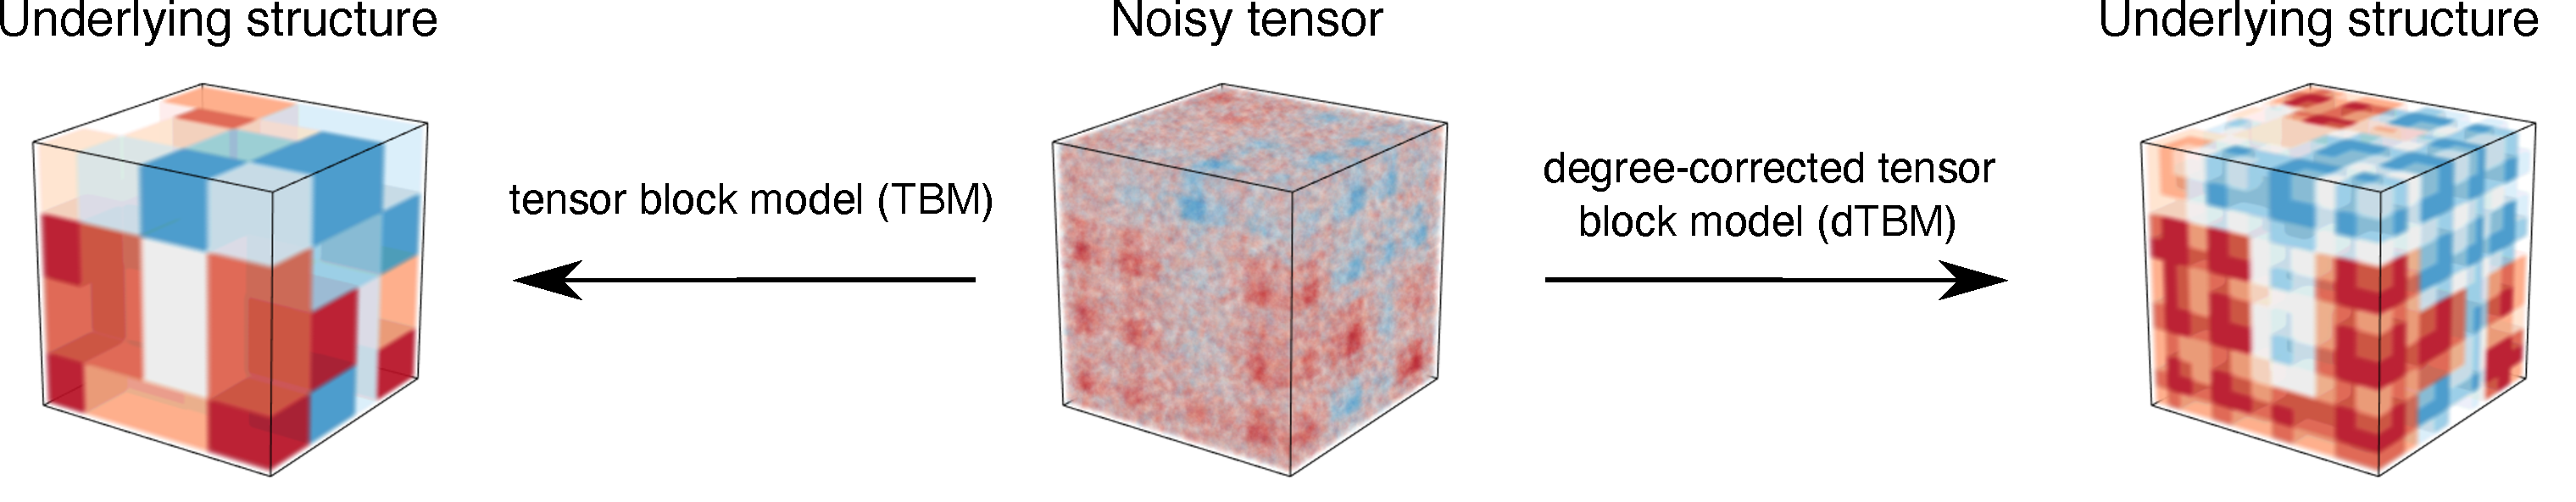
\includegraphics[width = .9\textwidth]{intro2_arxiv.pdf}
    \caption{Examples for order-3 tensor block model (TBM) with and without degree correction. Both TBM and dTBM have four communities on each mode, while dTBM allows a richer structure with degree heterogeneity.
    }
    \label{fig:intro}
\end{figure*}

{\bf Our contributions.} The primary goal of this paper is to provide both statistical and computational guarantees for dTBM. Our main contributions are summarized below.
\begin{itemize}[leftmargin=*]

 \item We develop a general dTBM and establish the identifiability for the uniqueness of clustering using the notion of angle separability.
 
\item  We present the phase transition of clustering performance with respect to three different statistical and computational behaviors.  We characterize, for the first time, the critical signal-to-noise (SNR) thresholds in dTBMs, revealing the intrinsic distinctions among (vector) one-dimensional clustering, (matrix) biclustering, and (tensor) higher-order clustering. Specific SNR thresholds and algorithm behaviors are depicted in  Figure~\ref{fig:phase_axis}. 
        
 \item We provide an angle-based algorithm that achieves exact clustering \emph{in polynomial time} under mild conditions. Simulation and data studies demonstrate the outperformance of our algorithm compared with existing higher-order clustering algorithms. 
\end{itemize}
The last two contributions, to our best knowledge, are new to the literature of dTBMs. 



\begin{figure*}[t]
    \centering
    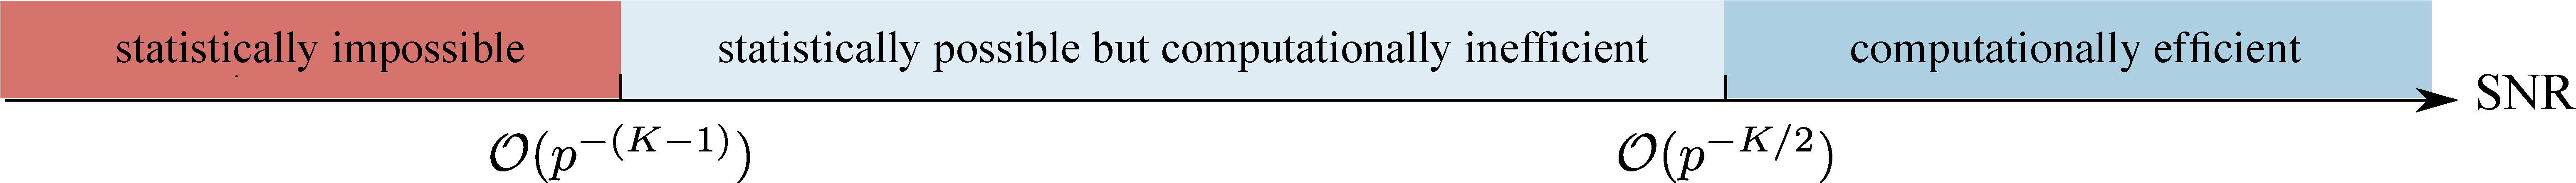
\includegraphics[width = 17cm]{phase.pdf}
    \caption{SNR thresholds for statistical and computational limits in order-$K$ dTBM with dimension $(p,...,p)$ and $K \geq 2$. The SNR gap between statistical possibility and computational efficiency  exists only for tensors with $K \geq 3$. }
    \label{fig:phase_axis}
\end{figure*}




{\bf Related work.} 
Our work is closely related to but also distinct from several lines of existing research. Table~\ref{tab:comp} summarizes the most relevant models. 

\begin{itemize}[wide]
    \item \textit{Block model for clustering.} Block models such as stochastic block model (SBM) and degree-corrected SBM have been widely used for matrix clustering problems. The theoretical properties and algorithm performance for matrix block models have been well-studied~\citep{gao2018community}; see the review paper~\citep{abbe2017community} and the references therein. However, The tensor counterparts are relatively less understood. 
    
    \item  \textit{Tensor block model.} The (non-degree) tensor block model (TBM) is a higher-order extension of SBM, and its statistical-computational properties are investigated in recent literatures~\citep{wang2019multiway, han2020exact, ghoshdastidar2017consistency}. Extending results from non-degree to degree-corrected model is highly challenging. Our dTBM parameter space is equipped with angle-based similarity and nuisance degree parameters. The extra complexity makes the Cartesian coordinates based analysis~\citep{han2020exact} non-applicable to our setting. Towards this goal, we have developed a new polar coordinates based analysis to control the model complexity. We also develop a new angle-based iteration algorithm to achieve optimal clustering rates \emph{without the need of estimating nuisance degree parameters}.
    
    
    \item \textit{Degree-corrected block model.} The hypergraph degree-corrected block model (hDCBM) and its variant have been proposed in the literature~\citep{ke2019community, yuan2018testing}. For this popular model, however, the optimal statistical-computational rates remain an open problem. Our main contribution is to provide a sharp statistical and computational critical phase transition in dTBM literature. In addition, our algorithm results in a faster \emph{exponential} error rate, in contrast to the \emph{polynomial} rate in~\cite{ke2019community}. The original hDCBM~\citep{ke2019community} is designed for binary observations only, and we extend the model to both continuous and binary observations. We believe our results are novel and helpful to the community. See Fig~\ref{fig:phase_axis} for overview of our results. 
    
    \item \textit{Global-to-local algorithm strategy.} Our methods generalize the recent global-to-local strategy for matrix learning~\citep{gao2018community,chi2019nonconvex,yun2016optimal} to tensors~\citep{han2020exact,ahn2018hypergraph,kim2018stochastic}. Despite the conceptual similarity, we address several fundamental challenges associated with this non-convex, non-continuous problem. We show the insufficiency of the conventional tensor HOSVD~\citep{de2000multilinear}, and we develop a weighted higher-order initialization that relaxes the singular-value gap separation condition. Furthermore, our local iteration leverages the angle-based clustering in order to avoid explicit estimation of degree heterogeneity. Our bounds reveal the interesting interplay between the computational and statistical errors. We show that our final estimate \emph{provably} achieves the exact clustering within only polynomial-time complexity. 
    
\end{itemize}



\begin{table*}[t]
\resizebox{\textwidth}{!}{%
    \begin{tabular}{c|ccccc}
\hline
    & \cite{gao2018community}&  \cite{han2020exact}&  \cite{ghoshdastidar2017consistency} &\cite{ke2019community} & \textbf{Ours}\\
    \hline
      Allow tensors of arbitrary order & $\times$ & $\surd$ & $\surd$ &$\surd$ & $\surd$  \\
        Allow degree heterogeneity &  $\surd$ & $\times$ & $\surd$ &$\surd$ & $\surd$ \\
        Singular-value gap-free clustering &  $\surd$ & $\surd$ & $\times$ & $\times$ &$\surd$ \\
        Misclustering rate (for order $K^*$)& - & $\exp(-p^{K/2})$ & $p^{-1}$& $p^{-2}$ &  $\exp(-p^{K/2})$\\
        \hline
    \end{tabular}
    }
    \caption{Comparison between previous methods with our method. $^*$We list the result for order-K tensors with $K \geq 3$ and general number of communities $r = \tO(1)$. }\label{tab:comp}
\end{table*}

{\bf Notation.} We use lower-case letters (e.g., $a,b$) for scalars, lower-case boldface letters (e.g., $\ma,\mtheta$) for vectors, upper-case boldface letters (e.g., $\mX,\mY$) for matrices, and calligraphy letters (e.g., $\tX,\tY$) for tensors of order three or greater. We use $\mone_p$ to denote a vector of length $p$ with all entries to be 1. We use $|\cdot|$ for the cardinality of a set and $\ind\{\cdot\}$ for the indicator function. For an integer $p\in\mathbb{N}_{+}$, we use the shorthand $[p]= \offf{1,2,...,p}$. For a length-$p$ vector $\ma$, we use $a(i)\in\mathbb{R}$ to denote the $i$-th entry of $\ma$, and use $\ma_{I}$ to denote the sub-vector by restricting the indices in the set $I\subset [p]$.  We use  $\onorm{\ma}=\sqrt{\sum_{i}a^2(i)}$ to denote the $\ell_2$-norm, $\onorm{\ma}_1=\sum_i |a_i|$ to denote the $\ell_1$ norm of $\ma$. For two vector $\ma, \mb$ of the same dimension, we denote the angle between $\ma, \mb$ by 
\begin{equation}
    \cos \of{\ma, \mb} = \frac{\ang{ \ma, \mb}}{ \onorm{\ma} \onorm{\mb} },
\end{equation}
where $\ang{\ma,\mb}$ is the inner product of two vectors and $\cos \of{\ma, \mb} \in [-1,1]$. We make the convention that $\cos \of{\ma, \mb} = \cos \of{\ma^T, \mb^T}$. 

Let $\tY  \in \bbR^{p_1 \times \cdots \times p_K}$ be an order-$K$ $(p_1,...,p_K)$-dimensional tensor. We use $\tY(i_1,\ldots,i_K)$ to denote the $(i_1,\ldots,i_K)$-th entry of $\tY$. The multilinear multiplication of a tensor $\tS\in \bbR^{r_1\times \cdots \times r_K}$ by matrices $\mM_k \in\mathbb{R}^{p_k\times r_k}$ results in an order-$d$ $(p_1,\ldots,p_K)$-dimensional tensor $\tX$, denoted
\[
\tX=\tS \times_1 \mM_1 \times \cdots \times_K \mM_K,
\]
where the entries of $\tX$ are defined by
\begin{align}
    &\tX(i_1,\ldots, i_K)=\sum_{(j_1,\ldots,j_K)}\tS(j_1,\ldots,j_K)\mM_1(i_1,j_1)\cdots \mM_K(i_K,j_K).
\end{align} 
For a matrix $\mY$, we use $\mY_{i:}$ (respectively, $\mY_{:i}$) to denote the $i$-th row (respectively, $i$-th column) of the matrix. Similarly, for an order-3 tensor, we use $\tY_{::i}$ to denote the $i$-th matrix slide of the tensor. We use $\text{Ave}(\cdot)$ to denote the operation of taking averages across elements and $\text{Mat}_k(\cdot)$ to denote the unfolding operation that reshapes the tensor along mode $k$ into a matrix. For a symmetric tensor $\tY\in\mathbb{R}^{p\times \cdots \times p}$, we omit the subscript and use $\text{Mat}(\tY)\in\mathbb{R}^{p\times p^{K-1}}$ to denote the unfolding. For two sequences $\{a_p\}, \{b_p\}$, we denote $a_p\lesssim b_p$ or $a_p=\tO(b_p)$ if $\lim_{p\to\infty}a_p /b_p\leq c$ for some constant $c\geq 0$, $a_p=o(b_p)$ if $\lim_{p\to\infty}a_p/b_p =0$, and $a_p = \Omega(b_p)$ if both $b_p \lesssim a_p$ and $a_p\lesssim b_p$. Throughout the paper, we use the terms ``community'' and ``clusters'' exchangeably. 


{\bf Organization.} The rest of this paper is organized as follows. Section~\ref{sec:model} introduces the degree-corrected tensor block model (dTBM) with three motivating examples and presents the identifiability of dTBM under the angle gap condition. We show the phase transition and the existence of statistical-computational gaps for the higher-order dTBM in Section~\ref{sec:limits}. In Section~\ref{sec:alg}, we provide a polynomial-time two-stage algorithm with misclustering rate guarantees. Numerical studies including the simulation, comparison with other methods, and two real dataset analyses are in Sections~\ref{sec:simulation}-\ref{sec:real}. The main technical ideas we develop for addressing main theorems are provided in Section~\ref{sec:mainproof}. Detailed proofs and extra theoretical results are provided in Appendix.


\section{Model formulation and motivations}\label{sec:model}

\subsection{Degree-corrected tensor block model}

Suppose we have an order-$K$ data tensor $\tY \in \bbR^{p \times \cdots \times p}$. For ease of notation, we focus on symmetric tensors in this section; the extension to general asymmetric tensors is provided in Section~\ref{subsec:exten}. Assume there exist $r \geq 2$  disjoint communities among the $p$ nodes. We represent the community assignment by a function $z \colon [p]\mapsto[r]$, where $z(i) = a$ for $i$-th node that belongs to the $a$-th community. Then, $z^{-1}(a)=\{i\in[p]\colon z(i)=a\}$ denotes the set of nodes that belong to the $a$-th community, and $|z^{-1}(a)|$ denotes the number of nodes in the $a$-th community. Let $\mtheta=(\theta(1),\ldots,\theta(p))^T$ denote the degree heterogeneity for $p$ nodes. We consider the order-$K$ dTBM~\citep{ghoshdastidar2017consistency,ke2019community},
\begin{equation}\label{eq:model_margin}
    \tY(i_1,\ldots,i_K) = \tS(z(i_1),\ldots,z(i_K)) \prod_{k = 1}^K\theta_{i_k} + \tE(i_1,\ldots,i_K), 
\end{equation}
\normalsize
where $\tS \in \bbR^{r \times \cdots \times r}$ is an order-$K$ tensor collecting the block means among communities, and $\tE\in\mathbb{R}^{p\times \cdots \times p}$ is a noise tensor consisting of independent zero-mean sub-Gaussian entries with variance bounded by $\sigma^2$. The unknown parameters are $z$, $S$, and $\mtheta$. The dTBM can be equivalently written in a compact form of tensor-matrix product:
\begin{equation}\label{eq:model_tensor}
\bbE\tY = \tS \times_1 \mTheta \mM \times_2 \cdots \times_K  \mTheta \mM,
\end{equation}
where $\mTheta = \text{diag}(\theta(1),...,\theta(p)) \in \bbR^{p \times p}$ is a diagonal matrix, $\mM \in \offf{0,1}^{p \times r}$ is the membership matrix associated with community assignment $z$ such that $\mM(i,j)=\ind\{z(i)=j\}$. By definition, each row of $\mM$ has one copy of 1's and 0's elsewhere. Note that the discrete nature of $\mM$ renders our model~\eqref{eq:model_tensor} more challenging than Tucker decomposition. We call a tensor $\tY$ an $r$-block tensor with degree $\mtheta$ if $\tY$ admits dTBM~\eqref{eq:model_tensor}. The goal of clustering is to estimate $z$ from a single noisy tensor $\tY$. We are particularly interested in the high-dimensional regime where $p$ grows whereas $r=\tO(1)$. 


\subsection{Motivating examples} Here, we provide four applications to illustrate the practical necessity of dTBM.

\vspace{0.2cm}
\paragraph{Tensor block model} Consider the model~\eqref{eq:model_tensor}. Let $\theta(i)=1$ for all $ i \in [p]$. The model~\eqref{eq:model_tensor} reduces to the tensor block model, which is widely used in previous clustering algorithms~\citep{wang2019multiway,chi2020provable,han2020exact}. The theoretical results in TBM serve as benchmarks for dTBM.  

\vspace{0.2cm}

\paragraph{Community detection in hypergraphs} Hypergraph network is a powerful tool to represent the complex entity relations with higher-order interactions~\citep{ke2019community}. A typical undirected hypergraph is denoted as $H = (V,E)$, where $V = [p]$ is the set of nodes and $E$ is the set of undirected hyperedges. Each hyperedge in $E$ is a subset of $V$, and we call the hyperedge an order-$K$ edge if the corresponding subset involves $K$ nodes. We call $H$ a $K$-uniform hypergraph if $E$ only contains order-$K$ edges. 

It is natural to represent the $K$-uniform hypergraph using a binary order-$K$ adjacency tensor. Let $\tY \in \{0,1\}^{p \times \cdots \times p}$ denote the adjacency tensor, where the entries encode the presence or absence of order-$K$ edges among $p$ nodes. Specifically, for all $(i_1,\ldots,i_K) \in [p]^K$, we have
\begin{equation}
    \tY(i_1,...,i_K) =  \begin{cases}
    1  & \text{if }  (i_1,...,i_K) \in E,\\
    0 & \text{if }  (i_1,...,i_K) \notin E.
    \end{cases}
\end{equation}


Assume there exist $r$ disjoint communities among $p$ nodes, and the connection probabilities depend on the community assignments and node-specific parameters. 
Then, the equation~\eqref{eq:model_tensor} models $\bbE \tY$ with unknown degree heterogeneity $\mtheta$ and sub-Gaussianity parameter $\sigma^2 = 1/4$.  

\vspace{0.2cm}
\paragraph{Multi-layer weighted network} 
Multi-layer weighted network data consists of multiple networks over the same set of nodes. One representative example is the brain connectome data~\citep{zhang2019tensor}. The multi-layer weighted network $\tY$ has dimension of $p \times p \times L$, where $p$ denotes the number of brain regions of interest, and $L$ denotes the number of layers (networks). Each of the $L$ networks describes one aspect of the brain connectivity, such as functional connectivity or structural connectivity. The resulting tensor $\tY$ consists of a mixture of slices with various data types. 


Assume there exist $r$ disjoint communities among $p$ nodes and $r_l$ disjoint communities among the $L$ layers. The multi-layer network community detection is modeled by the generalized asymmetric dTBM model~\eqref{eq:model_tensor}
\begin{equation}
    \bbE \tY = \tS \times_1 \mTheta \mM \times_2 \mTheta \mM \times_3 \mTheta_l \mM_l, 
\end{equation}
where $(\mtheta \in \bbR^p, \mM \in \{0,1\}^{p \times r})$ and $ (\mtheta_l \in \bbR^L, \mM_l \in \{0,1\}^{L \times r_l})$ are the degree heterogeneity and membership matrices corresponding to the community structure for $p$ nodes and $L$ layers, respectively. 
\vspace{0.2cm}

\paragraph{Gaussian higher-order clustering} Datasets in various fields such as medical image, genetics, and computer science are formulated as Gaussian tensors. One typical example is the multi-tissue gene expression dataset, which records the different gene expression in different individuals and different tissues. The dataset, denoted as $\tY \in \bbR^{p \times n \times t}$, consists of the expression data for $p$ genes of $n$ individuals in $t$ tissues. 

Assume there exist $r_1, r_2, r_3$ disjoint clusters for $p$ genes, $n$ individuals, and $t$ tissues, respectively. We apply the generalized asymmetric dTBM model~\eqref{eq:model_tensor} 
\begin{equation}
    \bbE\tY = \tS \times_1 \mTheta_1 \mM_1 \times_2 \mTheta_2 \mM_2 \times_3 \mTheta_3 \mM_3, 
\end{equation}
where $\{(\mtheta_k, \mM_k)\}_{k=1}^3$ represents the heterogeneity and membership for genes, individuals, and tissues. \\


\begin{rmk}[Comparison with non-degree models]
Our dTBM uses fewer block parameters than TBM. In particular, every non-degree $r_1$-block tensor can be represented by a \emph{degree-corrected} $r_2$-block tensor with $r_2\leq r_1$. In particular, there exist tensors with $r_1=p$ but $r_2=1$, so the reduction in model complexity can be dramatic from $p$ to 1. This fact highlights the benefits of introducing degree heterogeneity in higher-order clustering tasks.
\end{rmk}


\subsection{Identifiability under angle gap condition}
The goal of clustering is to estimate the partition function $z$ from model~\eqref{eq:model_tensor}. For ease of notation, we focus on symmetric tensors; the extension to non-symmetric tensors are similar. We use $\tP$ to denote the following parameter space for $(z,\tS,\mtheta)$,
\begin{align}\label{eq:family}
\tP=\bigg\{(z,\tS,\mtheta)\colon  \ \mtheta\in\mathbb{R}^p_{+},\ 
{c_1p\over r}\leq |z^{-1}(a)|\leq {c_2 p\over r}, c_3\leq \onormSize{}{\text{Mat}(\tS)_{a:}}\leq c_4, \onorm{\mtheta_{z^{-1}(a)}}_1=|z^{-1}(a)|, a\in[r]\bigg\},
\end{align}
\normalsize
where $c_i>0$'s are universal constants. We briefly describe the rationale of the constraints in~\eqref{eq:family}. 
First, the entrywise positivity constraint on  $\mtheta\in\mathbb{R}^p_{+}$ is imposed to avoid sign ambiguity between entries in $\mtheta_{z^{-1}(a)}$ and $\tS$. This constraint allows the trigonometric $\cos$ to describe the angle similarity in the Assumption~\ref{assmp:min_gap} below and Sub-algorithm~\hyperref[alg:main]{2} in Section~\ref{sec:alg}. Note that the positivity constraint can be achieved without sacrificing model flexibility, by using a slightly larger dimension of $\tS$ in the factorization~\eqref{eq:model_tensor}; see Example~\ref{ex:positive} below. Second, recall that the quantity $|z^{-1}(a)|$ denotes the number of nodes in $a$-th community. The constants $c_1, c_2$ in the $|z^{-1}(a)|$ bound assume the roughly balanced size across $r$ communities. Third, the constants $c_3, c_4 $ in the magnitude of $\text{Mat}(\tS)_{a:}$ requires no purely zero slide in $\tS$, so the core tensor $\tS$ is not trivially reduced to a lower rank. Lastly, the $\ell_1$ normalization $\onormSize{}{\mtheta_{z^{-1}(a)}}_1=|z^{-1}(a)|$ is imposed to avoid the scalar ambiguity between $\mtheta_{z^{-1}(a)}$ and $\tS$. This constraint, again, incurs no restriction to model flexibility but makes our presentation cleaner. 

\begin{example}[Positivity of degree parameters]~\label{ex:positive}
Here we provide an example to show the positivity constraints on $\mtheta$ incurs no loss on the model flexibility. 
Consider an order-3 dTBM with core tensor $\tS = 1$ and degree $\mtheta = (1,1,-1, -1)^T$. We have the mean tensor 
\begin{equation}
    \tX = \tS \times_1 \mTheta \mM \times_2 \mTheta \mM \times_3 \mTheta \mM,
\end{equation}
where $\mTheta = \text{diag}(\mtheta)$ and $\mM = (1,1,1,1)^T$. Note that $\tX \in \bbR^{4 \times 4 \times 4}$ is a 1-block tensor with \emph{mixed-signed} degree $\mtheta$, and the mode-3 slices of $\tX$ are
\begin{equation}
    \tX_{::1} = \tX_{::2} = - \tX_{::3} = -\tX_{::4}  = \begin{bmatrix}
    1 & 1& -1& -1 \\
    1 & 1& -1& -1 \\
    -1& -1&1 & 1\\
     -1& -1&1 & 1
    \end{bmatrix}.
\end{equation}
Now, instead of original decomposition, we encode $\tX$ as a 2-block tensor with \emph{positive-signed} degree. Specifically, we write
\begin{equation}
     \tX = \tS' \times_1 \mTheta' \mM' \times_2 \mTheta' \mM'  \times_3 \mTheta' \mM' , 
\end{equation}
where $\mTheta' = \text{diag}(\mtheta') = \text{diag}(1,1, 1, 1)$, the core tensor $\tS' \in \bbR^{2 \times 2 \times 2}$ has mode-3 slices, and the membership matrix $\mM'\in\{0,1\}^{4\times 2}$ defines the clustering $z'\colon[4]\to[2]$,
\begin{equation}
    \tS'_{::1} = -\tS'_{::2} = \begin{bmatrix}
    1 & -1 \\
    -1 & 1
    \end{bmatrix}, \quad \mM' = \begin{bmatrix}
   1 & 0 \\
   1 &0 \\
    0 & 1 \\
    0&1
    \end{bmatrix}.
\end{equation}
 The triplet $(z',\tS', \mtheta')$ lies in our parameter space~\eqref{eq:family}. In general, we can always reparameterize a block-$r$ tensor with mixed-signed degree using a block-$2r$ tensor with positive-signed degree. Since we assume $r=\tO(1)$ throughout the paper, the splitting does not affect the error rates of our interest.\end{example}

We now provide the identifiability conditions for our model before estimation procedures. When $r=1$, the decomposition~\eqref{eq:model_tensor} is always unique (up to cluster label permutation) in $\tP$, because dTBM is equivalent to the rank-1 tensor family under this case. When $r\geq 2$, the Tucker rank of signal tensor $\bbE\tY$ in~\eqref{eq:model_tensor} is bounded by, but not necessarily equal to, the number of blocks $r$~\citep{wang2019multiway}. Therefore, one can not apply the classical identifiability conditions for low-rank tensors to dTBM. Here, we introduce a key separation condition on the core tensor. 

\begin{assumption}[Angle gap] \label{assmp:min_gap}Let $\mS = \text{Mat}(\tS)$. Assume the minimal gap between normalized rows of $\mS$ is bounded away from zero; i.e.,
\begin{equation}\label{eq:minimal_gap}
    \Delta_{\min} := \min_{a \neq b \in [r]} \onorm{\frac{\mS_{a:}}{\onormSize{}{ \mS_{a:}}} - \frac{\mS_{b:}}{\onormSize{}{ \mS_{b:}}} }>0, \quad \text{for} \quad r \geq 2.
\end{equation}
\end{assumption}
We make the convention $\Delta_{\min} = 1$ for $r = 1$. Equivalently, \eqref{eq:minimal_gap} says that none of the two rows in $\mS$ are parallel; i.e., $\max_{a \neq b\in [r]}\cos \of{\mS_{a:},\  \mS_{b:}}  = 1-\Delta^2_{\min}/2<1$. The quantity $\Delta_{\min}$ characterizes the non-redundancy among clusters measured by angle separation. The denominators involved in definition~\eqref{eq:minimal_gap} are well posed because of the lower bound on $\onorm{\mS_{a:}}$ in~\eqref{eq:family}. 

Our first main result is the following theorem showing the sufficiency and necessarily of the angle gap separation condition for the parameter identifiability under dTBM. 

\begin{thm}[Model identifiability]\label{thm:unique} Consider the dTBM with $r\geq 2$. The parameterization~\eqref{eq:model_tensor} is unique in $\tP$ up to cluster label permutations, if and only if Assumption~\ref{assmp:min_gap} holds.
\end{thm}

The identifiability guarantee for the dTBM is more appealing than classical Tucker model. In the Tucker model, the factor matrix $\mM$ is identifiable only up to orthogonal rotations. In contrast, our model does not suffer from rotational invariance. As we will show in Section~\ref{sec:alg}, each column of the membership matrix $\mM$ can be precisely recovered under our algorithm. This property benefits the interpretation of dTBM in practice. 

\section{Statistical-computational limits for higher-order tensors}\label{sec:limits}

In this section, we study the statistical and computational limits of dTBM. We propose signal-to-noise ratio~(SNR),
\begin{align}\label{eq:gamma}
  \text{SNR}:= \Delta^2_{\min}/\sigma^2 = p^{\gamma}, 
\end{align}
with varying $\gamma \in \bbR$ that quantifies different regimes of interest. We call $\gamma$ the \emph{signal exponent}. Intuitively, a larger SNR, or equivalently a larger $\gamma$, benefits the clustering in the presence of noise. With quantification~\eqref{eq:gamma}, we consider the following parameter space,
\begin{equation}\label{eq:gammafamily}
    \tP(\gamma) = \tP\cap\{\tS \text{ satisfies SNR condition~\eqref{eq:gamma} with $\gamma$} \}.
\end{equation}
Note that $1$-block dTBM does not belong to the space $\tP(\gamma)$ when $\gamma < 0$ by Assumption~\ref{assmp:min_gap}. Our goal is to characterize the clustering accuracy with respect to $\gamma$. Let $\hat z$ and $z$ be the estimated and true clustering functions in the family~\eqref{eq:family}. Define the misclustering error by
\[
\ell(\hat z, z)={1\over p}\min_{\pi \in \Pi}\sum_{i\in[p]}\ind\{\hat z(i)\neq \pi \circ z(i)\},
\]
where $\pi: [r] \mapsto [r]$ is a permutation of cluster labels, $\circ$ denotes the composition operation, and $\Pi$ denotes the collection of all possible permutations. The infinitum over all permutations accounts for the ambiguity in cluster label permutation. 

In Sections~\ref{sec:statlimit} and \ref{sec:complimit}, we provide the lower bounds of $\ell (\hat z, z)$ for general Gaussian dTBMs~\eqref{eq:model_margin} without symmetric assumptions. For general (asymmetric) Gaussian dTBMs, we assume Gaussian noise $\tE(i_1,\ldots,i_K)\stackrel{\text{i.i.d.}}{\sim} N(0,\sigma^2)$, and we extend the parameter space~\eqref{eq:family} to allow $K$ clustering functions $(z_k)_{k\in[K]}$, one for each mode. For notational simplicity, we still use $z$ and $\tP(\gamma)$ for this general (asymmetric) model. All lower bounds should be interpreted as the worst-case results across $K$ modes. 


\subsection{Statistical critical values}\label{sec:statlimit}
The statistical limit means the minimal SNR required for solving dTBMs with \emph{unlimited computational cost.} Our following result shows the minimax lower bound of SNR for exact recovery in dTBM. 

\begin{thm}[Statistical lower bound]\label{thm:stats} Consider general Gaussian dTBMs under the parameter space $\tP(\gamma)$ with $K\geq 1$. Assume $r \lesssim p^{1/3}$. If the signal exponent satisfies $\gamma < -(K-1)$, then, every estimator $\hat z_{\text{stat}}$ obeys
\begin{equation}
    \sup_{(z, \tS, \mtheta) \in \tP(\gamma)} \bbE \left[ p\ell(\hat z_{\text{stat}}, z) \right]\geq 1.
\end{equation}
\end{thm}
Theorem~\ref{thm:stats} demonstrates the impossibility of exact recovery of the assignment when $\gamma < -(K-1)$ in the high-dimensional regime $p\to \infty$ for fixed $r$. The proof is information-theoretical, and therefore the results apply to all statistical estimators, including but not limited to, maximum likelihood estimation (MLE)~\citep{wang2019multiway} and trace maximization~\citep{ghoshdastidar2017uniform}. As we will show in Section~\ref{sec:alg}, the SNR threshold $-(K-1)$ is also a minimax upper bound, because MLE achieves exact recovery when $\gamma > -(K-1)$. Hence, the boundary $\gamma_{\text{stat}} \coloneqq -(K-1)$ is the critical value for statistical performance of dTBM. 


\subsection{Computational critical values}\label{sec:complimit}
In this section, we derive the computational limits of dTBMs. The computational limit means the minimal SNR required for exactly recovery with \emph{polynomial-time} computational cost. An important ingredient to establish the computational limits is the \emph{hypergraphic planted clique (HPC) conjecture} \citep{zhang2018tensor, brennan2020reducibility}. The HPC conjecture indicates the impossibility of fully recovering the planted cliques with polynomial-time algorithm when the clique size is less than the number of vertices in the hypergraph. The formal statement of HPC detection conjecture is provided in Definition~\ref{def:HPC} and Conjecture~\ref{hypo:HPC} as follows.  


\begin{defn}[Hypergraphic planted clique (HPC) detection]~\label{def:HPC} Consider an order-$K$ hypergraph $H = (V,E)$ where $V = [p]$ collects vertices and $E$ collects all the order-$K$ edges. Let $\tH_k(p, 1/2)$ denote the Erd\H{o}s-R\'{e}nyi $K$-hypergraph where the edge $(i_1,\ldots, i_K)$ belongs to $E$ with probability $1/2$. Further, we let $\tH_K(p, 1/2, \kappa)$ denote the hyhpergraph with planted cliques of size $\kappa$. Specifically, we generate a hypergraph from $\tH_k(p, 1/2)$, pick $\kappa$ vertices uniformly from $[p]$, denoted $K$, and then connect all the hyperedges with vertices in $K$. Note that the clique size $\kappa$ can be a function of $p$, denoted $\kappa_p$. The order-$K$ HPC detection aims to identify whether there exists a planted clique hidden in an Erd\H{o}s-R\'{e}nyi $K$-hypergraph. The HPC detection is formulated as the following hypothesis testing problem
\begin{equation}
    H_0:\ H \sim \tH_K(p,1/2) \quad \text{versus} \quad H_1: \ H \sim \tH_K(p,1/2, \kappa_p).
\end{equation}
\end{defn}

\begin{conjecture}[HPC conjecture]\label{hypo:HPC} Consider the HPC detection problem in Definition~\ref{def:HPC}. Suppose the sequence $\{\kappa_p\}$ such that $\limsup_{p \rightarrow \infty} \log \kappa_p/ \log \sqrt{p} \leq (1 - \tau)$. Then, for every sequence of polynomial-time test $\{ \varphi_p\}: H \mapsto \{0,1\}$ we have 
\begin{equation}
    \liminf_{p \rightarrow \infty} \bbP_{H_0} \of{ \varphi_p(H) =1 } +  \bbP_{H_1} \of{ \varphi_p(H) =0} \geq \frac{1}{2}.
\end{equation}
\end{conjecture}

Under the HPC conjecture, we establish the SNR lower bound that is necessary for any \emph{polynomial-time} estimator to achieve exact clustering.

\begin{thm}[Computational lower bound]\label{thm:comp} Consider general Gaussian dTBMs under the parameter space $\tP(\gamma)$ with $K\geq 2$. Assume HPC conjecture holds. If the signal exponent $\gamma < -K/2$, then, every \emph{polynomial-time estimator} $\hat z_{\text{comp}}$ obeys
\begin{align}
   \liminf_{p\to \infty}\sup_{(z, \tS, \mtheta) \in \tP(\gamma)}  \bbE \left[ p\ell(\hat z_{\text{comp}}, z) \right]\geq 1.
\end{align}
\end{thm}
Theorem~\ref{thm:comp} indicates the impossibility of exact recovery by polynomial-time algorithms when $\gamma < -K/2$.  Therefore, $\gamma_{\text{comp}}:=-K/2$ is the critical value for computational performance of dTBM.  In Section~\ref{sec:alg}, we will show the condition $\gamma> -K/2$ suffices for our proposed polynomial-time estimator. Thus, $\gamma_{\text{comp}}:=-K/2$ is the critical value for computational performance of dTBM.  

\begin{rmk}[Statistical-computational gaps]
Now, we have established the phase transition of exact clustering under order-$K$ dTBM by combing Theorems~\ref{thm:stats} and \ref{thm:comp}. Figure~\ref{fig:phase_axis} summarizes our results of critical SNRs when $K \geq 2$. In the weak SNR region $\gamma < -(K-1)$, no statistical estimator succeeds in degree-corrected higher-order clustering. In the strong SNR region $\gamma  > -K/2$, our proposed algorithm precisely recovers the clustering in polynomial time. In the moderate SNR regime, $-(K-1)\leq \gamma \leq -K/2$, the degree-corrected clustering problem is statistically easy but computationally hard. Particularly, dTBM reduces to matrix degree-corrected model when $K =2$, and the statistical and computational bounds show the same critical value. When $K =1$, dTBM reduces to the degree-corrected sub-Gaussian mixture model (GMM) with model
\begin{equation}
    \mY = \mTheta \mM \mS + \mE,
\end{equation}
where $\mY \in \bbR^{p \times d}$ collects $n$ data points in $\bbR^d$, $\mS \in \bbR^{r \times d}$ collects the $d$-dimensional centroids for $r$ clusters, and $\mTheta \in \bbR^{p \times p}, \mM \in \{0,1\}^{p \times r}, \mE \in \bbR^{p \times d}$ have the same meaning as in dTBM. \cite{lu2016statistical} implies that polynomial-time algorithms are able to achieve the statistical minimax lower bound in GMM. Therefore, we conclude that the statistical-to-computational gap emerges only for higher-order tensors with $K \geq 3$. The result reveals the intrinsic distinctions among (vector) one-dimensional clustering, (matrix) biclustering, and (tensor) higher-order clustering. 
\end{rmk}


\begin{rmk}[Comparison with non-degree models]
We compare our results to non-degree tensor models. The allowance of degree heterogeneity $\mtheta$ makes the model more flexible, but it incurs extra statistical and computational complexity. Fortunately, we find that the extra complexity does not render the estimation of $z$ qualitatively harder; see the comparison of our phase transition with non-degree TBM~\citep{han2020exact}. 
\end{rmk}



\section{Polynomial-time algorithm under mild SNR}\label{sec:alg}
In this section, we present an efficient polynomial-time clustering algorithm under mild SNR. The procedure takes a global-to-local approach. See Figure~\ref{fig:demo} for illustration. The global step finds the basin of attraction with polynomial miclustering error, whereas the local iterations improve the initial clustering to exact recovery. Both steps are critical to obtain a satisfactory algorithm output. In what follows, we first use the symmetric tensor as a working example to describe the algorithm procedures to gain insight. Our theoretical analysis focuses on the noisy tensor with i.i.d.\ sub-Gaussian noise such as Gaussian and uniform observations. The extensions for asymmetric tensor and Bernoulli observation and other practical issues are in Section~\ref{subsec:exten}.

\begin{figure}[ht!]
\centering
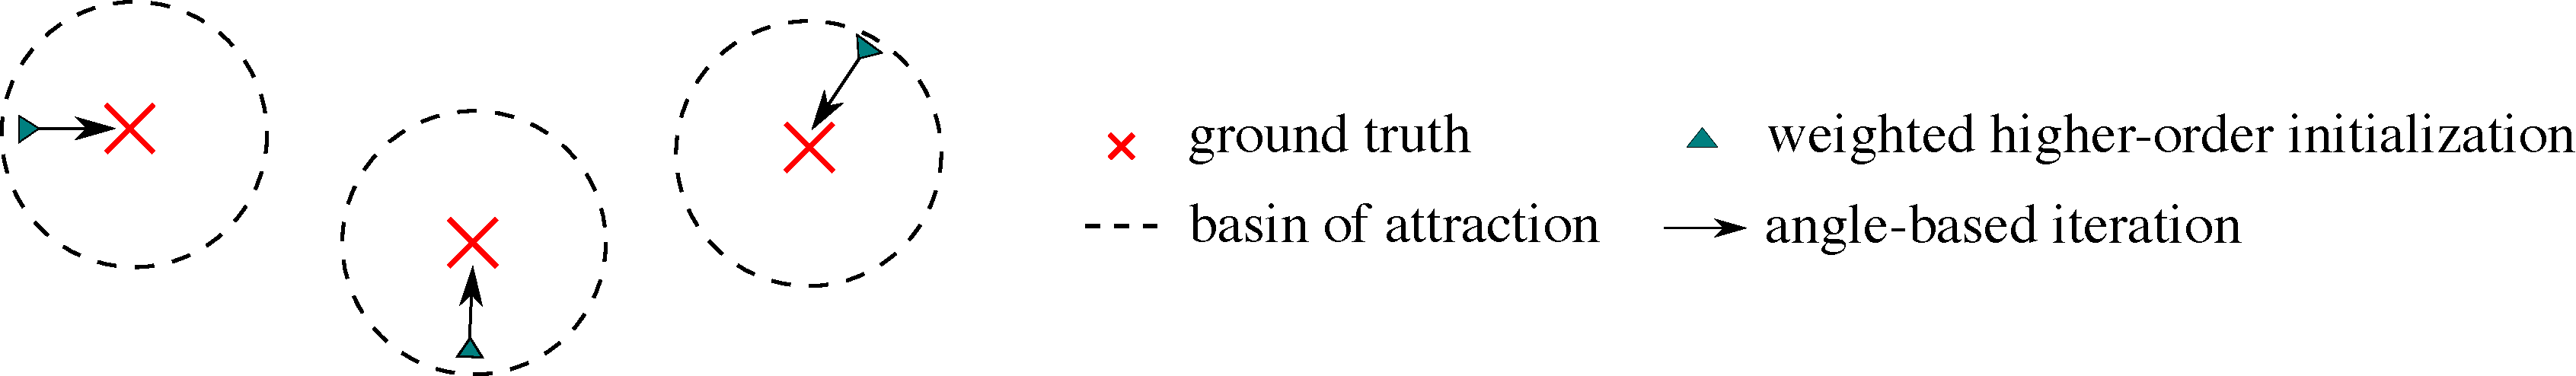
\includegraphics[width=\columnwidth]{alg_demo1.pdf}
\caption{Illustration of our global-to-local algorithm.}\label{fig:demo}
\end{figure}

\subsection{Weighted higher-order initialization}

We start with weighted higher-order clustering algorithm as initialization. We take an order-3 symmetric tensor as illustration for insight. Consider noiseless case with $\tX = \bbE\tY$ and $\mX = \text{Mat}(\tX)$. 
By model~\eqref{eq:model_tensor}, for all $i \in [p]$, we have
\begin{equation}\label{eq:kmeans}
    \theta(i)^{-1} \mX_{i:} = \off{\text{Mat}( \tS \times_2 \mTheta \mM \times_3  \mTheta \mM )}_{z(i):}. 
\end{equation}
This implies that, all node $i$ belonging to $a$-th community (i.e., $z(i)=a$) share the same normalized mean vector $\theta(i)^{-1} \mX_{i:}$, and vice versa. Intuitively, one can apply $k$-means clustering to the vectors $\{ \theta(i)^{-1} \mX_{i:} \}_{i\in[p]}$, which leads to main idea of our Sub-algorithm~\hyperref[alg:main]{1}.  


Specifically, our initialization consists of denoising step and clustering step. The denoising step (lines 1-2 in Sub-algorithm~\hyperref[alg:main]{1}) estimates $\tX$ from $\tY$ by a double projection spectral method.  
The first projection performs HOSVD~\citep{de2000multilinear} via $\mU_{\text{pre}} = \text{SVD}_{r} \of{ \text{Mat}(\tY) }$, where $\text{SVD}_r(\cdot)$ returns the top-$r$ left singular vectors. The second projection performs HOSVD on the projected $\tY$ onto the multilinear Kronecker space $\mU_{\text{pre}} \otimes  \mU_{\text{pre}}$; i.e.,
\begin{equation}\label{eq:two-step_factor}
    \hat \mU = \text{SVD}_{r} \of{\text{Mat}\of{ \tY\times_1  \mU_{\text{pre}} \mU_{\text{pre}}^T \times_2   \mU_{\text{pre}} \mU_{\text{pre}}^T }}.
\end{equation}
The final denoised tensor $\hat \tX$ is defined by
\begin{equation}\label{eq:two-step_est}
    \hat \tX = \tY \times_1 \hat \mU \hat 
\mU^T \times_2 \hat \mU \hat \mU^T \times_3 \hat \mU \hat \mU^T. 
\end{equation}
The double projection improves usual matrix spectral methods in order to alleviate the noise effects for $K\geq 3$~\citep{han2020exact}.

The clustering step (lines 3-5 in Sub-algorithm~\hyperref[alg:main]{1}) performs the weighted $k$-means clustering. 
We write $\hat \mX=\text{Mat}(\hat \tX)$, and normalize the rows into $\hat \mX^s_{i:}=\onormSize{}{\hat \mX_{i:}}^{-1}\hat \mX_{i:}$ as a surrogate of $\theta(i)^{-1} \mX_{i:}$. Then, a weighted $k$-means clustering is performed on the normalized rows with weights equal to $\onormSize{}{\hat \mX_{i:}}^2$. The choice of weights is to bound the $k$-means objective function by the Frobenius-norm accuracy of $\hat \tX$. Unlike existing clustering algorithm~\citep{ke2019community}, we apply the clustering on the unfolded tensor $\hat \mX$ rather than on the factors $\hat \mU$. This strategy relaxes the singular-value gap condition~\citep{gao2018community, han2020exact}.
We assign degenerate rows with purely zero entries to an arbitrarily random cluster; these nodes are negligible in high-dimensions because of the lower bound on $\onormSize{}{\text{Mat}(\tS)_{a:}}$ in~\eqref{eq:family}. The final result gives the initial cluster assignment $\hat z^{(0)}$. Full procedures are provided in Sub-algorithm~\hyperref[alg:main]{1}. 



\begin{algorithm}[h!]
\caption*{\bf Algorithm: Multiway spherical clustering for degree-corrected tensor block model }
\vspace{.15cm}
\begin{algorithmic}[1]
\Algphase{Sub-algorithm 1: Weighted higher-order initialization}
\INPUT Observation $\tY \in \bbR^{p\times \cdots \times p}$, cluster number $r$, relaxation factor $\eta > 1$ in $k$-means clustering.
\State Compute factor matrix $ \mU_{\text{pre}} = \text{SVD}_{r} (\text{Mat}(\tY))$ and the $(K-1)$-mode projection $
\tX_{\text{pre}} = \tY \times_1   \mU_{\text{pre}} \mU_{\text{pre}}^T \times_2 \cdots \times_{K-1}  \mU_{\text{pre}} \mU_{\text{pre}}^T.$
\State Compute factor matrix $\hat \mU = \text{SVD}_{r}(\text{Mat}(\tX_{\text{pre}}))$ and denoised tensor
$\hat \tX = \tY \times_1 \hat \mU \hat \mU^T \times_2 \cdots \times_K \hat \mU \hat \mU^T.$
\State {Let $\hat \mX = \text{Mat}(\hat \tX)$ and $S_0=\{i \in [p]: \onormSize{}{\hat \mX_{i:}} = 0\}$. Set $\hat z(i)$ randomly in $[r]$ for $i \in S_0$.}
\State{For all $i\in S_0^c$, compute normalized rows
$\hat \mX_{i:}^s :=\onormSize{}{\hat \mX_{i:}}^{-1} \hat \mX_{i:}.$
}
\State {Solve the clustering $\hat z\colon [p]\to[r]$ and centroids $ (\hat \mx_j)_{j\in[r_k]}$ using weighted $k$-means, such that}
\begin{align}
    &\sum_{i \in S_0^c }  \onormSize{}{\hat \mX_{i:}}^2 \onormSize{}{\hat \mX_{i:}^s - \hat \mx_{\hat z(i)} }^2 
    \leq 
    \eta \min_{\substack{\bar \mx_j, j\in[r], \bar z(i),i\in S_0^{c}}} \sum_{i \in S^c } \onormSize{}{\hat \mX_{i:}}^2 \onormSize{}{ \hat \mX_{i:}^s -   \bar \mx_{\bar z(i)}}^2.
\end{align}
\OUTPUT Initial clustering $z^{(0)} \leftarrow \hat z$.

\Algphase{Sub-algorithm 2: Angle-based iteration}
\INPUT Observation $\tY \in \bbR^{p \times \cdots \times p}$, initialization $z^{(0)} \colon [p]\to[r]$ from Sub-algorithm 1, iteration number $T$.
\For {$t = 0$ to $T-1$}
\State Update the block tensor $\tS^{(t)}$ via
$\tS^{(t)} (a_1,...,a_K)= \text{Ave} \{\tY(i_1,\ldots,i_K): z^{(t)}(i_k) = a_k, k \in [K]\}.$
\State Calculate reduced tensor $\tY^{\text{d}} \in \bbR^{p \times r \times \cdots \times r}$ via
\begin{align}
    &\tY^{\text{d}}(i,a_2,\ldots,a_K) 
    = 
\text{Ave}\{\tY(i,i_2,\ldots,i_K): z^{(t)}(i_k) = a_k, k \neq 1 \}.
\end{align}

\State Let $\mY^{\text{d}} = \text{Mat}(\tY^{\text{d}})$ and $J_0 = \{ i\in[p]: \onorm{\mY^{\text{d}}_{i:}} = 0\}$. Set $z^{(t+1)}(i)$ randomly in $[r]$ for $i \in J_0$.

\State Let $\mS^{(t)} = \text{Mat}(\tS^{(t)})$. For all $i \in J_0^c$ update the cluster assignment by
\begin{equation}
    z(i)^{(t+1)} = \argmax_{a \in [r]} \cos \left( \mY^{\text{d}}_{i:},\ \mS^{(t)}_{a:} \right).
\end{equation}

\EndFor

\OUTPUT Estimated clustering $z^{(T)}  \in [r]^{p}$.

\end{algorithmic}
\end{algorithm}

We now establish the misclustering error rate of initialization. We call $\mtheta$ is balanced, if the relative extent of heterogeneity is comparable across clusters in that
\begin{equation}\label{eq:degree}
{\min_{a\in[r]} \onormSize{}{\mtheta_{z^{-1}(a)}}=\left(1+o(1)\right)\max_{a\in[r]}\onormSize{}{\mtheta_{z^{-1}(a)}}}.
\end{equation}
Note that, the assumption~\eqref{eq:degree} does not preclude degree heterogeneity. Indeed, within each of the clusters, the highest degree can be $\theta(i) = \Omega(p)$, whereas the lowest degree can be $\theta(i)=\tO(1)$. 

\begin{thm}[Error for weighted higher-order initialization]\label{thm:initial} Consider the general sub-Gaussian dTBM with i.i.d.\ noise under the parameter space $\tP$ and Assumption~\ref{assmp:min_gap}. Assume $\mtheta$ is balanced and $\min_{i\in[p]}\theta(i) \geq c$ for some constant $c>0$. Let $ z^{(0)}$ denote the output of Sub-algorithm~\hyperref[alg:main]{1}. With probability going to 1, we have
\begin{equation}\label{eq:ini}
   \ell(z^{(0)}, z) \lesssim {r^K p^{-K/2}\over \text{SNR}}. 
\end{equation}
\end{thm}

\begin{rmk}[Comparison to previous results] For fixed SNR, our initialization error rate with $K=2$ agrees with the initialization error rate $\tO(p^{-1})$ in matrix models~\citep{gao2018community}. Furthermore, in the special case of non-degree TBMs with $\theta_1=\cdots=\theta_p=1$, we achieve the same initial misclustering error $\tO(p^{-K/2})$ as in non-degree models~\citep{han2020exact}. Theorem~\ref{thm:initial} implies the advantage of our algorithm in achieving both accuracy and model flexibility. 
\end{rmk}



\begin{rmk}[Failure of conventional tensor HOSVD] If we use conventional HOSVD for tensor denoising; that is, we use $\mU_{\text{pre}}$ in place of $\hat \mU$ in line 2, then the misclustering rate becomes $\tO(p^{-1})$ for all $K\geq 2$. This rate is substantially worse than our current rate~\eqref{eq:ini}.
\end{rmk}


\begin{rmk}[Singular-value gap-free clustering] Note that our clustering directly applies to the estimated mean tensor $\hat \tX$ rather than the leading tensor factors $\hat \mU$. Applying clustering to the tensor factors suffers from the non-identifiability issue due to the infinitely many orthogonal rotations when the number of blocks $r \geq 3$ in the absence of singular-value gaps. 
Such ambiguity causes the trouble for effective clustering~\citep{abbe2020entrywise}. In contrast, our initialization algorithm applies the clustering to the overall mean tensor $\hat \tX$. This strategy avoids the non-identifiability issue regardless of the number of blocks and singular-value gaps.  
\end{rmk}


\subsection{Angle-based iteration}
Our Theorem~\ref{thm:initial} has shown the polynomially decaying error rate from our initialization. Now we improve the error rate to exponential decay using local iterations. We propose an angle-based local iteration to improve the outputs from Sub-algorithm~\hyperref[alg:main]{1}. 
To gain the intuition, consider an one-dimensional degree-corrected clustering problem with data vectors $\mx_i = \theta(i) \ms_{z(i)} + \mepsilon_i, i \in [p]$, where $\ms_i$'s are known cluster centroids, $\theta(i)$'s are unknown positive degrees, and $z\colon [p] \mapsto [r]$ is the cluster assignment of interest. The angle-based $k$-means algorithm estimates the assignment $z$ by minimizing the angle between data vectors and centroids; i.e., 
 \begin{equation}\label{eq:angle_kmeans}
     z(i) = \argmax_{a \in [r]} \cos ( \mx_i,\ \ms_{a} ),\ \text{ for all }i \in [p].
 \end{equation}
The classical Euclidean-distance based clustering~\citep{han2020exact} fails to recover $z$ in the presence of degree heterogeneity, even under noiseless case. In contrast, the proposed angle-based $k$-means achieves accurate recovery without explicit estimation of $\mtheta$. 

Our Sub-algorithm~\hyperref[alg:main]{2} shares the same spirit as in angle-based $k$-means. We still take the order-3 tensor for illustration. Specifically, Sub-algorithm~\hyperref[alg:main]{2} updates estimated core tensor and cluster assignment in each iteration. We use superscript $\cdot^{(t)}$ to denote the estimate from $t$-th iteration, where $t=1,\ldots.$ For core tensor, we consider the following update strategy  
 \[
 \tS^{(t)}(a_1,a_2,a_3)=\text{Ave}\{\tY(i_1,i_2,i_3)\colon z^{(t)}(i_k)=a_k, k\in[3]\}.
\]
Intuitively, $\tS^{(t)}$ becomes closer to the true core $\tS$ as $z^{(t)}$ is more precise. For cluster assignment, we first aggregate the slices of $\tY$ and obtain a reduced tensor $\tY^{\text{d}}\in \bbR^{p \times r \times r}$ with given $z^{(t)}$, where
\[
\tY^{\text{d}}(i,a_2,a_3)=\text{Ave}\{\tY(i,i_2,i_3)\colon z^{(t)}(i_k)=a_k, k \neq 1\}.
\]
We use $\mY^d$ and $ \mS^{(t)}$ to denote the $\text{Mat}(\tY^{\text{d}})$ and $\text{Mat}(\tS^{(t)})$. The rows $\mY^d_{i:}$ and $\mS^{(t)}_{a:}$ correspond to the $\mx_i$ and $\ms_a$ in the one-dimensional clustering~\eqref{eq:angle_kmeans}. Then, we obtain the updated assignment by
\[
z(i)^{(t+1)} = \argmax_{a \in [r]} \cos \of{ \mY^{\text{d}}_{i:}, \mS^{(t)}_{a:} },\ \text{ for all } i \in [p],
\]
provided that $\mS^{(t)}_{a:}$ is a non-zero vector. Otherwise, if $\mS^{(t)}_{a:}$ is a zero vector, then we make the convention to assign $z^{(t+1)}(i)$ randomly in $[p]$. Full procedures for our angle-based iteration are described in Sub-algorithm~\hyperref[alg:main]{2}. 

We now establish the misclustering error rate of iterations under the stability assumption.

\begin{defn}[Locally linear stability] \label{def:stable}
Define the $\varepsilon$-neighborhood of $z$ by $\tN(z,\epsilon)=\{\bar z\colon \ell(\bar z, z)\leq \epsilon\}$. Let $\bar z\colon[p]\to [r]$ be a clustering function. We define two vectors associated with $\bar z$,
\begin{align}
    &\mp(\bar z)=(|\bar z^{-1}(1)|, \ldots,|\bar z^{-1}(r)|)^T, \quad \mp_{\mtheta}(\bar z)=(\onormSize{}{\mtheta_{\bar z^{-1}(1)}}_1,\ldots,\onormSize{}{\mtheta_{\bar z^{-1}(r)}}_1)^T.
\end{align}

We call the degree is $\varepsilon$-locally linearly stable if and only if 
\begin{equation}\label{eq:local}
    \sin(\mp(\bar z),\ \mp_{\mtheta}(\bar z))\lesssim \varepsilon \Delta_{\min} ,\quad \text{for all } \bar z\in \tN(z, \varepsilon).
\end{equation}
\end{defn}

Roughly speaking, the vector $\mp(\bar z)$ represents the raw cluster sizes, and $\mp_{\theta}(\bar z)$ represents the relative cluster sizes weighted by degrees. 
The local stability holds trivially for $\varepsilon=0$ based on the construction of parameter space~\eqref{eq:family}. The condition~\eqref{eq:local} controls the impact of node degree to the $\mp_{\theta}(\cdot)$ with respect to the misclassification rate $\varepsilon$ and angle gap.
 
\begin{thm}[Error for angle-based iteration]\label{thm:refinement} Consider the setup as in Theorem~\ref{thm:initial}. Assume the local linear stability of degree holds in the neighborhood $\tN(z,\epsilon)$ for $\epsilon \geq \log^{-1}p$. Suppose 
$r=\tO(1)$ and $\text{SNR} \geq \tilde C p^{-K/2}\log p$ for some sufficiently large constant $\tilde C$. Let $z^{(t)}$ denote the $t$-th iteration output in Sub-algorithm~\hyperref[alg:main]{2} with initialization $z^{(0)}$ from Sub-algorithm~\hyperref[alg:main]{1}. With probability going to 1, there exists a contraction parameter $\rho \in (0,1)$ such that 
\begin{align}\label{eq:final}
    \ell(z, \hat z^{(t+1)}) \lesssim &\ \KeepStyleUnderBrace{
   \text{SNR}^{-1}
    \exp\of{- \frac{p^{K-1}\text{SNR}}{r^{K-1}}}}_{\substack{\text{statistical error}} }+ \KeepStyleUnderBrace{ \rho^t \ell(z, z^{(0)}). }_{\substack{\text{computational error}}}
\end{align}
\end{thm}
From the conclusion~\eqref{eq:final}, we find that the iteration error is decomposed into two parts: statistical error and computational error. The statistical error is unavoidable with noisy data regardless $t$, whereas the computational error decays in an exponential rate as the number of iterations $t \rightarrow \infty$. 

Theorem~\ref{thm:refinement} implies that, with probability going to 1, our estimate $z^{(T)}$ achieves exact recovery within polynomial iterations; more precisely,
\begin{equation}
     z^{(T)} = \pi \circ z, \quad \text{for all }T\gtrsim \log_{1/\rho} p,
\end{equation}
for some permutation $\pi \in \Pi$. Therefore, our combined algorithm is \textit{computationally efficient} as long as SNR $\gtrsim p^{-K/2} \log p$. Note that, ignoring the logarithmic term, the minimal SNR requirement, $p^{-K/2}$, coincides with the computational lower bound in Theorem~\ref{thm:comp}. Therefore, our algorithm is optimal regarding the signal requirement and lies in the sharpest \emph{computationally efficient} regime in Figure~\ref{fig:phase_axis}.


\subsection{Extensions and practical issues}~\label{subsec:exten}
\hspace{-.3cm} {\bf Extension for Bernoulli observations.} The main difficulty to establish the statistical guarantee for Bernoulli observations lies in the initialization Sub-algorithm~\hyperref[alg:main]{1}. Theorem~\ref{thm:refinement} still holds for Bernoulli observations once the initialization accuracy satisfies the upper bound~\eqref{eq:ini} in Theorem~\ref{thm:initial}.

We now provide a high-level explanation for the technical difficulty when applying Theorem~\ref{thm:initial} to Bernoulli observations. The derivation of Theorem~\ref{thm:initial} relies on the upper bound of the estimation error for the mean tensor in Lemma~\ref{lem:two-step_esterror}; i.e., with high probability
\begin{equation}\label{eq:prop1}
    \onormSize{}{\hat \tX - \tX}_F^2 \lesssim p^{K/2},
\end{equation}
where $\tX = \bbE\tY$ and $\hat \tX$ is defined in Step 2 of Sub-algorithm~\hyperref[alg:main]{1}. Unfortunately, the inequality~\eqref{eq:prop1} holds only for i.i.d.\ sub-Gaussian observations while Bernoulli observations are generally not identically distributed.  

One possible remedy is to apply singular value decomposition to the \emph{square unfolding}~\citep{mu2014square} of Bernoulli tensor $\tY$. Let the matrix $\mat_{sq} (\tY) \in \{0,1\}^{\floor{p^{K/2}} \times \ceil{p^{K/2}} }$ denote the nearly square unfolded Bernoulli tensor. Define a new estimate 
\begin{equation}\label{eq:matrixsvd}
    \hat \tX' = \argmin_{\text{rank}(\mat_{sq}(\tX)) \leq r^{\ceil{K/2}}} \onormSize{}{ \mat_{sq}(\tX) -  \mat_{sq}(\tY)}_F^2.
\end{equation}
The optimization~\eqref{eq:matrixsvd} is simply a matrix SVD problem. Following Lemma 7 in \cite{gao2018community}, with high probability, the new estimate satisfies
\begin{equation}
    \onormSize{}{\hat \tX' - \tX}_F^2 \lesssim p^{\ceil{K/2}}.
\end{equation} 
Replacing the estimate $\hat \tX$ by $\hat \tX'$ in Theorem~\ref{thm:initial}, the high probability upper bound for Bernoulli initialization is
\begin{equation}\label{eq:ini_b}
    \ell(z^{(0)}, z) \lesssim \frac{r^K p^{- \floor{K/2} }}{\text{SNR}}. 
\end{equation}
The Bernoulli bound~\eqref{eq:ini_b} is relatively looser than Gaussian bound~\eqref{eq:ini}, especially when $K$ is small. Nevertheless, our bound~\eqref{eq:ini_b} is already tighter than the pervious work~\citep{ke2019community}. The investigation of the gap between upper bound $p^{- \floor{K/2}}$ and the lower bound $p^{- K/2}$ for Bernoulli tensors will be left as future work. 


{\bf Extension for general dTBMs.} Our two-stage algorithm is able to be extended for the general (asymmetric) dTBMs. Specifically, in the Sub-algorithm~\hyperref[alg:main]{1}, we make the following changes: (1)
Replace the matrcization $\mat(\tY)$ by $\mat_k(\tY)$; (2) Repeat the Steps 1-5 with mode-specified cluster number $r_k$; (3) Obtain the collection initialization $ \{z^{(0)}_k\}_{k=1}^K$. In the Sub-algorithm~\hyperref[alg:main]{2}, we make the following changes: (1) Take the collection $\{z^{(0)}_k\}_{k=1}^K$ as input, and update the block tensor $\tS^{(t)}$ with the collection $\{ z_k^{(t)}\}_{k=1}^K$, $
        \tS^{(t)}(a_1,\ldots, a_K) =  \text{Ave} \{\tY(i_1,\ldots,i_K): z^{(t)}_k(i_k) = a_k, k \in [K]\}$;
(2) Calculate reduced tensor $\tY^{\text{d}}_k$ for each mode via
\begin{align}
    &\tY^{\text{d}}_k(a_1,\ldots,a_{k-1}, i ,a_{k+1},\ldots,a_K) 
    = \text{Ave}\{\tY(i_1,\ldots,i_{k-1},i,i_{k+1},\ldots,i_K): z^{(t)}(i_j) = a_j, j \neq k \}; 
\end{align}

(3) Repeat Step 8-10 with $\mat_k(\cdot), \tY_k^{\text{d}}$ for each $k \in [K]$ and obtain the collection $\{z^{(T)}_k\}_{k=1}^K$. 

Correspondingly, Theorems~\ref{thm:initial} and \ref{thm:refinement} still hold with $\ell(z^{(0)}_k, z_k)$ and $\ell(z^{(t+1)}_k, z_k)$  for all $k \in [K]$. The detailed model extension for general asymmetric dTBMS can be found in Appendix. 

{\bf Computational complexity.} Our two-stage algorithm has a computational cost polynomial in tensor dimension $p$. Specifically, the complexity of Sub-algorithm~\hyperref[alg:main]{1} is $\tO(K p^{K+1} + Krp^K)$, where the first term is contributed by the double projection and the calculation of $\hat \tX$, and the second term comes from normalization and the $k$-means. The cost of each update in Sub-algorithm~\hyperref[alg:main]{2} is $\tO(p^K + pr^K)$, where $p^K$ comes from the calculation of $\tS^{(t)}$ and $\tY^{\text{d}}$, and $pr^K$ comes from the normalization of $\tY^{\text{d}}$, the calculation of $\tS^{(t)}$, and the cluster assignment update in Step 10.

{\bf Hyper-parameter selection.} In our theoretical analysis, we have assumed the true cluster number $r$ is given to our algorithm. In practice, the cluster number $r$ is often unknown, and we now propose a method to choose $r$ from data. We impose the Bayesian information criterion (BIC) and choose the cluster number that minimizes BIC; i.e., under the symmetric Gaussian dTBM~\eqref{eq:model_tensor},
\begin{align}\label{eq:BIC}
 \hat r &= \argmin_{r \in \mathbb{Z}_+ } \of{p^K \log(\onormSize{}{\hat \tX - \tY}_F^2)  + p_e(r) K \log p},\\
 \text{where}  \quad \hat \tX &= \hat \tS(r) \times_1 \hat \mTheta(r) \hat \mM(r) \times_2 \cdots \times_K \hat \mTheta(r) \hat \mM(r),
\end{align}
where the triplet $(\hat z(r), \hat \mS(r),\hat \mtheta(r))$ are estimated parameters with cluster number $r$, and $p_e (r)= r^K + p(\log r + 1) - r$ is the effective number of parameters. Note that we have added the argument $(r)$ to related quantities as functions of $r$. In particular, the estimate $\hat \mtheta(r)$ in~\eqref{eq:BIC} is obtained by first calculating the reduced tensor $\hat \tY^{\text{d}}$ with $\hat z(r)$, and then normalizing the row norms $\onormSize{}{\hat \mY_{i:}^{\text{d}}}$ to 1 in each cluster; i.e., 
\begin{equation}
 \hat \mtheta(r)=(\hat \theta(1,r),\ldots,\hat \theta(p,r))^T,\quad\text{where}\quad   \hat \theta(i,r) = \frac{\onormSize{}{\hat \mY^{\text{d}}(r)_{i:}}}{\sum_{j: \hat z(j,r) =  \hat z(i,r)} \onormSize{}{\hat \mY^{\text{d}}(r)_{j:}}},
\end{equation}
where $\hat \mY^{\text{d}}(r) = \mat(\hat \tY^{\text{d}}(r))$, $\hat \tY^{\text{d}}(r)(i,a_2,\ldots,a_K) =  \text{Ave}\{\tY(i,i_2,\ldots,i_K): \hat z(i_k, r) = a_k, k \neq 1 \}$, and $\hat z(i,r)$ denotes the community label for the $i$-th node with given cluster number $r$. We evaluate the performance of the BIC criterion in Section~\ref{subsec:num_theory}.


\section{Numerical studies}\label{sec:simulation}

 We evaluate the performance of the weighted higher-order initialization and angle-based iteration in this section. We report average errors and standard deviations across 30 replications in each experiment. Clustering accuracy is assessed by clustering error rate (CER, i.e., one minus rand index). Note that CER between $(\hat z, z)$ is equivalent to misclustering error $\ell(\hat z, z)$ up to constant multiplications~\citep{meilua2012local}, and a lower CER indicates a better performance.

We generate order-3 tensors with \emph{assortative}~\citep{gao2018community} core tensors to control SNR; i.e., we set $\tS_{aaa} = s_1$ for $a \in [r]$ and others be $s_2$, where $s_1 > s_2 > 0$. Let $\alpha = s_1/s_2$. We set $\alpha$ close to 1 such that $1-\alpha=o(p)$. In particular, we have $\alpha = 1 + \Omega(p^{\gamma/2})$ with $\gamma<0$ by Assumption~\ref{assmp:min_gap} and definition~\eqref{eq:gamma}. Hence, we easily adjust SNR via varying $\alpha$. Note that the assortative setting is proposed for simulations, and our algorithm is applicable for general tensors in practice. The cluster assignment $z$ is randomly generated with equal probability across  $r$ clusters for each mode. Without further explanation, we generate degree heterogeneity $\mtheta$ from absolute normal distribution by $\theta(i) = |X_i| + 1 - 1/\sqrt{2\pi}$ with $|X_i| \stackrel{\text{i.i.d.}}\sim N(0,1), i \in [p]$ and normalize $\mtheta$ to satisfy \eqref{eq:family}. Also, we set $\sigma^2 = 1$ for Gaussian data without further specification. 

\subsection{Verification of theoretical results}\label{subsec:num_theory}

The first experiment verifies  statistical-computational gap described in Section~\ref{sec:limits}. Consider the Gaussian model with $p = \{80, 100\}$, $r = 5$. We vary $\gamma $ in $ [-1.2, -0.4]$ and $[-2.1, -1.4]$ for matrix ($K=2$) and tensor $(K = 3)$ clustering, respectively. Note that finding MLE under dTBM is computationally intractable. We approximate MLE using an oracle estimator, i.e., the output of Sub-algorithm~\hyperref[alg:main]{2} initialized from true assignment. Figure~\ref{fig:phase}a shows that both our algorithm and oracle estimator start to decrease around the critical value $\gamma_{\text{stat}}  = \gamma_{\text{comp}}  = -1$ in matrix case. In contrast, Figure~\ref{fig:phase}b shows a significant gap in the phase transitions between the algorithm estimator and oracle estimator in tensor case. The oracle error rapidly decreases to 0 when $\gamma_{\text{stat}} = -2$, whereas the algorithm estimator tends to achieve exact clustering when $\gamma_{\text{comp}} = -1.5$. Figure~\ref{fig:phase} confirms the existence of the statistical-computational gap in our Theorems~\ref{thm:stats} and~\ref{thm:comp}. 


\begin{figure}[htb]
    \centering
    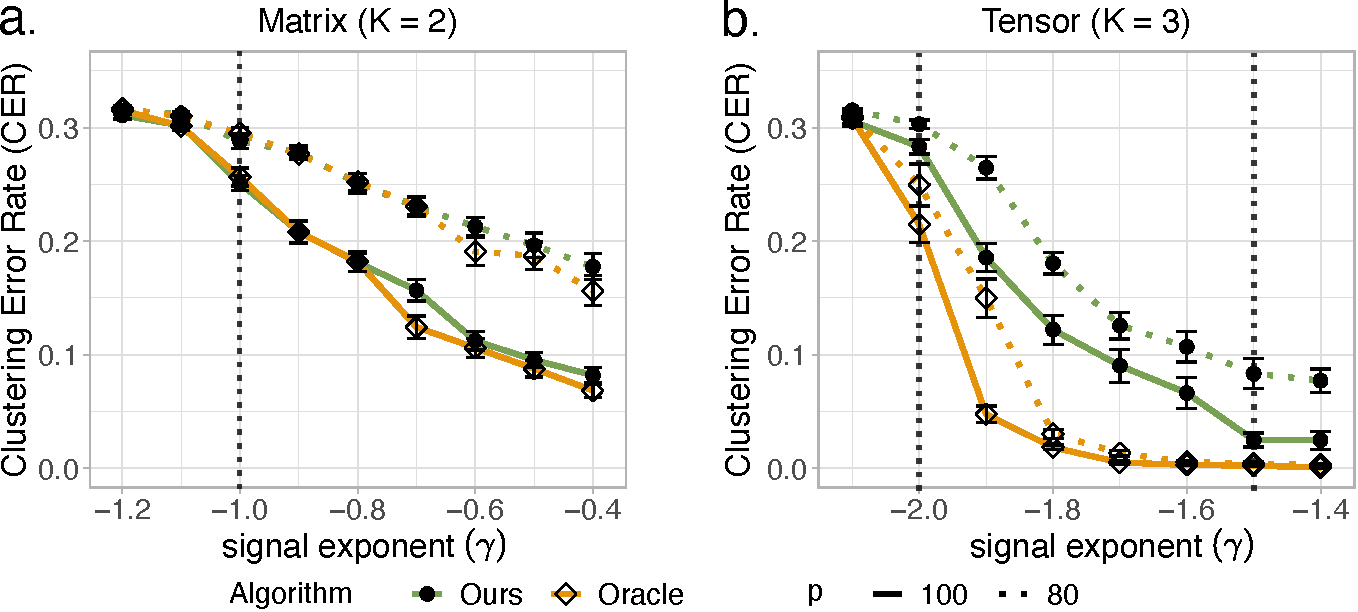
\includegraphics[width=.8\columnwidth]{phase_anno3.pdf}
    \caption{SNR phase transitions for clustering in dTBM with $p = \{80, 100\}, r = 5$ under (a) matrix case with $\gamma \in [-1.2, -0.4]$ and (b) tensor case with $ \gamma \in [-2.1, -1.4]$.
    }
    \label{fig:phase}
\end{figure}

The second experiment verifies the performance guarantees of two algorithms: (i) weighted higher-order initialization; (ii) combined algorithm of weighted higher-order initialization and angle-based iteration. We consider both the Gaussian and Bernoulli models with $p = \{80, 100\}$, $r = 5$, $\gamma \in [-2.1, -1.4]$. Figure~\ref{fig:ini_re} shows the substantial improvement of combined algorithm over initialization, especially under weak and intermediate signals. This phenomenon agrees with the error rates in Theorems~\ref{thm:initial} and \ref{thm:refinement} 
and confirms the necessity of the local iterations.

\begin{figure}[htp!]
    \centering
     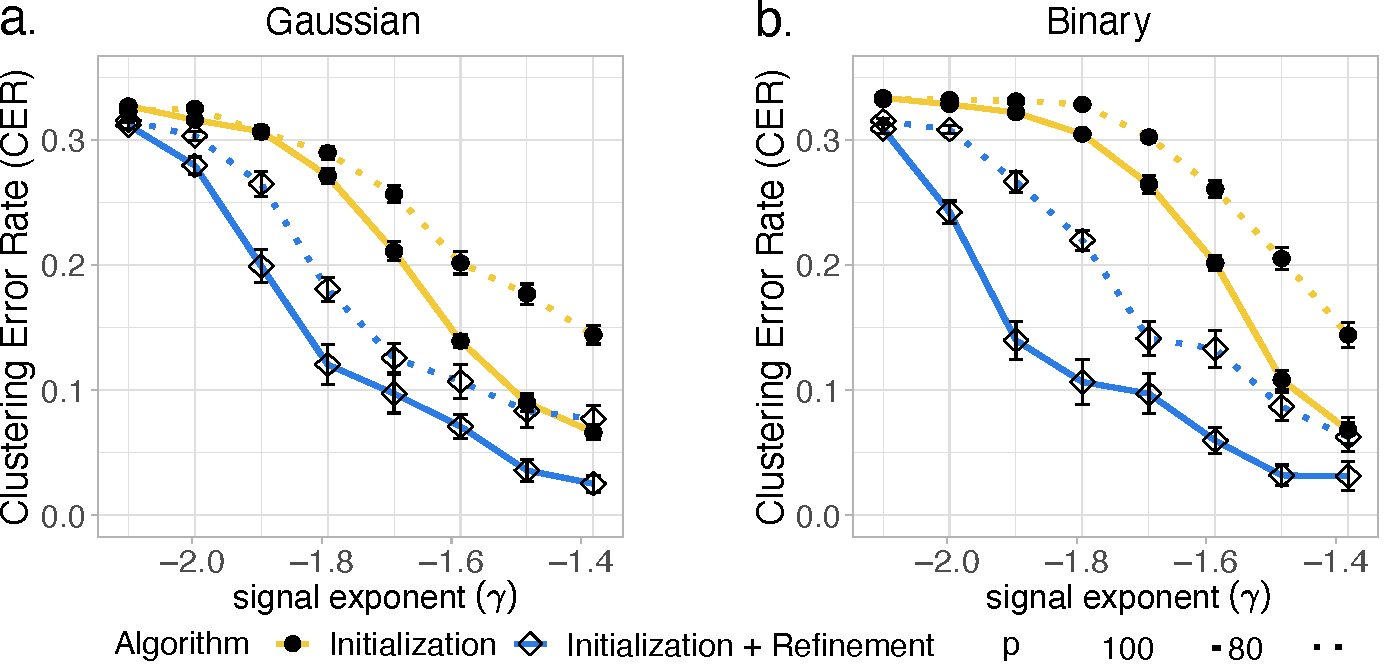
\includegraphics[width=.8\columnwidth]{ini_re_anno3.pdf}
    \caption{CER versus signal exponent $(\gamma)$ for initialization only and for combined algorithm. We set $p = \{80, 100\}, r = 5, \gamma \in [-2.1, -1.4]$ under (a) Gaussian models and (b) Bernoulli models. }
    \label{fig:ini_re}

\end{figure}


\begin{table}[hbt]
\centering
    \begin{tabularx}{\textwidth}{c *{8}{Y}}
    \toprule
    Settings & \multicolumn{2}{c}{$p = 50, \sigma^2 = 0.25$} & \multicolumn{2}{c}{$p = 50, \sigma^2 = 1$} & \multicolumn{2}{c}{$p = 80, \sigma^2 = 0.25$} & \multicolumn{2}{c}{$p = 80, \sigma^2 = 1$}\\
    \cmidrule(lr){2-3} \cmidrule(l){4-5} \cmidrule(l){6-7} \cmidrule(l){8-9}
         True cluster number $r$ & 2 & 4 & 2  & 4 & 2  & 4 & 2 & 4  \\
         \midrule
         Estimated cluster number $\hat r$ &  2(0)  & 3.9(0.25)& 2(0)    & 3.1(0.52) & 2(0)    & 4(0)   & 2(0)    & 3.9(0.31)   \\
     \bottomrule
    \end{tabularx}
    \caption{Estimated cluster number given by BIC criterion under the low noise level $(\sigma^2 = 0.25)$ and high noise level $(\sigma^2 = 0.5)$ settings. Numbers in parentheses are standard deviations of $\hat r$ over 30 replications.}
    \label{tab:select}
\end{table}

The third experiment evaluates the empirical performance of the BIC criterion to select unknown cluster number. We generate the data from an order-3 Gaussian model with $p = \{50,80\}$, $r = \{2,4\}$, and noise level $\sigma^2 \in \{ 0.25,1\}$. Table~\ref{tab:select} shows that our BIC criterion well chooses the true $r$ under most settings.  Note that the BIC slightly underestimates the true cluster number $(r = 4)$ with smaller dimension and higher noise $(p = 50, \sigma=1)$, and the accuracy immediately increases with larger dimension $p = 80$. The improvement follows from the fact that a larger dimension $p$ indicates a larger sample size in the tensor block model. Therefore, we conclude that BIC criterion is a reasonable way to tune the cluster number.


\subsection{Comparison with other methods}\label{subsec:comp}


We compare our algorithm with following higher-order clustering methods:
\begin{itemize}[wide,topsep=-3pt,itemsep=0pt,parsep=1pt]
    \item \textbf{\small HOSVD}: HOSVD on data tensor and $k$-means on the rows of the factor matrix;
    \item \textbf{\small HOSVD+}: HOSVD on data tensor and $k$-means on the $\ell_2$-normalized rows of the factor matrix;
    \item \textbf{\small HLloyd}~\citep{han2020exact}: High-order clustering algorithm developed for non-degree tensor block models;
    \item \textbf{\small SCORE}~\citep{ke2019community}: Tensor-SCORE for clustering developed for binary tensors.
\end{itemize}


Among the four alternative algorithms, the \textbf{\small SCORE} is the closest method to ours. We set the tuning parameters of \textbf{\small SCORE} as in previous literature \citep{ke2019community}. The methods \textbf{\small SCORE} and \textbf{\small HOSVD+} are designed for degree models, whereas \textbf{\small HOSVD} and \textbf{\small HLloyd} are designed for non-degree models. We conduct two experiments to assess the impacts of (i) signal strength and (ii) degree heterogeneity, based on Gaussian and Bernoulli models with $ p = 100, r = 5$. We refer to our algorithm as \textbf{\small dTBM} in the comparison. 

We investigate the effects of signal to clustering performance by varying $\gamma \in [-1.5, -1.1]$. Figure~\ref{fig:comp_gamma} shows the consistent outperformance of our method \textbf{\small dTBM} among all algorithms. The sub-optimality of \textbf{\small SCORE} and \textbf{\small HOSVD+} indicates the necessity of local iterations on the clustering. Furthermore,  Figure~\ref{fig:comp_gamma} shows the inadequacy of non-degree algorithms in the presence of mild degree heterogeneity. 
The experiment demonstrates the benefits of addressing heterogeneity in higher-order clustering tasks.   


\begin{figure}[h!]
    \centering
    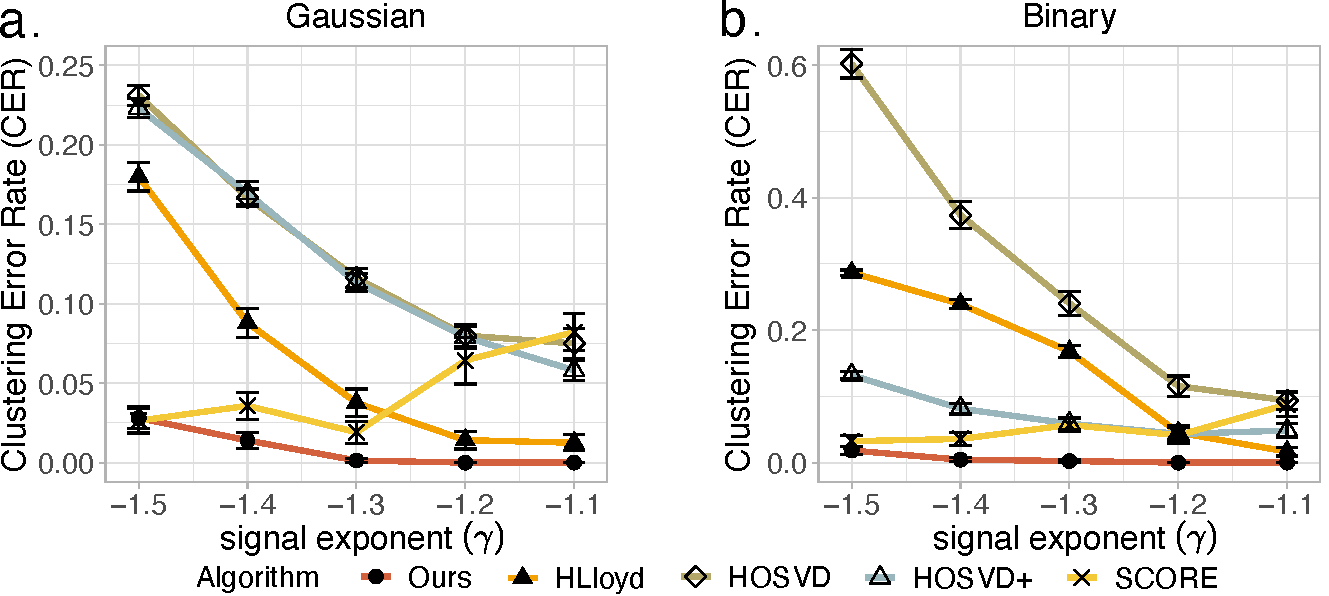
\includegraphics[width=.8\columnwidth]{comp_gamma_anno3.pdf}
    \caption{CER versus signal exponent (denoted $\gamma$) for different methods. We set $p = 100, r = 5, \gamma \in [-1.5, -1.1]$ under (a) Gaussian and (b) Bernoulli models.}
    \label{fig:comp_gamma}
\end{figure}


The only exception in Figure~\ref{fig:comp_gamma} is the slightly better performance of \textbf{\small HLloyd} over \textbf{\small HOSVD+} under Gaussian model. However, we find the advantage of \textbf{\small HLloyd} disappears with higher degree heterogeneity. We perform extra simulations to verify the impact of degree effects. We use the same setting as in the first experiment in the Section~\ref{subsec:comp}, except that we now generate the degree heterogeneity $\mtheta$ from Pareto distribution prior to normalization. The density function of Pareto distribution is $f(x|a,b) = a b^a x^{-(a+1)} \ind\{ x \geq b \}$, where $a$ is called \emph{shape} parameter. We vary $a \in \{2,6\}$ and choose $b$ such that $\bbE X = a(a - 1)^{-1}b = 1$ for $X$ following Pareto$(a,b)$. Note that a smaller $a$ leads to a larger variance in $\mtheta$ and hence a larger degree heterogeneity. We consider the Gaussian model under low $(a = 6)$ and high $(a = 2)$ degree heterogeneity. Figure~\ref{fig:comp_gamma_theta} shows that the errors for non-degree algorithms (\textbf{\small HLloyd}, \textbf{\small HOSVD}) increase with degree heterogeneity. In addition, the advantage of \textbf{\small HLloyd} over \textbf{\small HOSVD+} disappears with higher degree heterogeneity. 



\begin{figure}[h!]
    \centering
    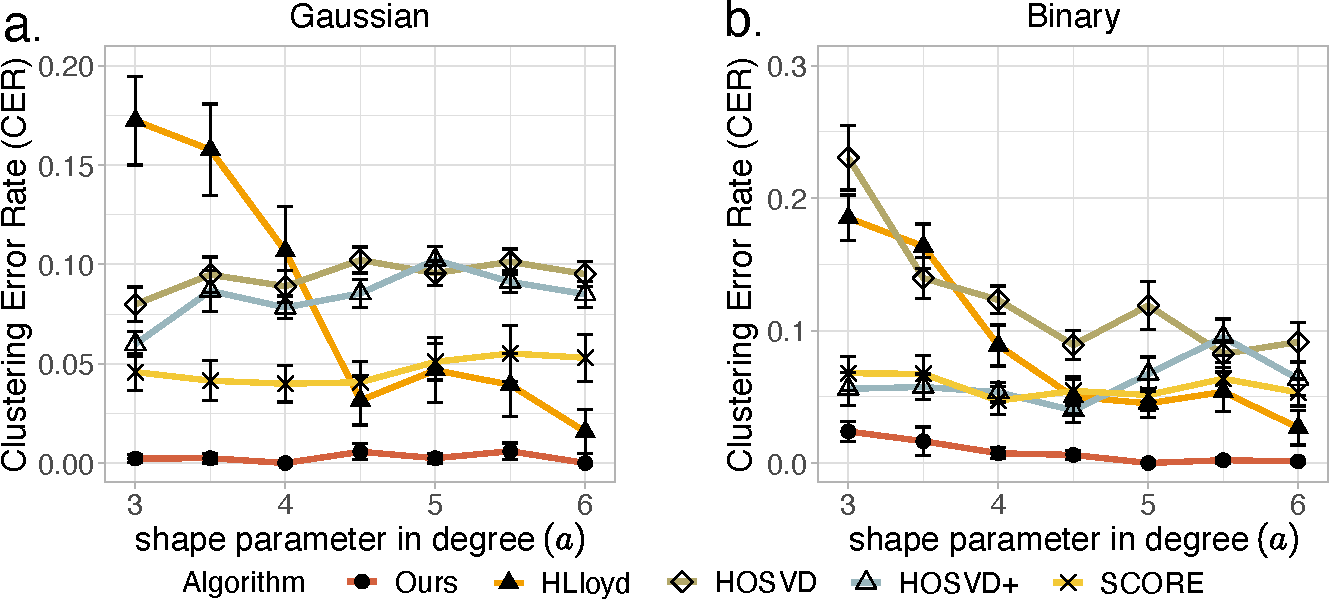
\includegraphics[width=.8\columnwidth]{comp_theta_anno3.pdf}
    \caption{CER versus shape parameter in degree (denoted $a\in[3,6]$) for different methods. We set $p = 100, r = 5, \gamma = -1.2$ under (a) Gaussian and (b) Bernoulli models.}
    \label{fig:comp_theta}
\end{figure}



\begin{figure}[htp!]
    \centering
    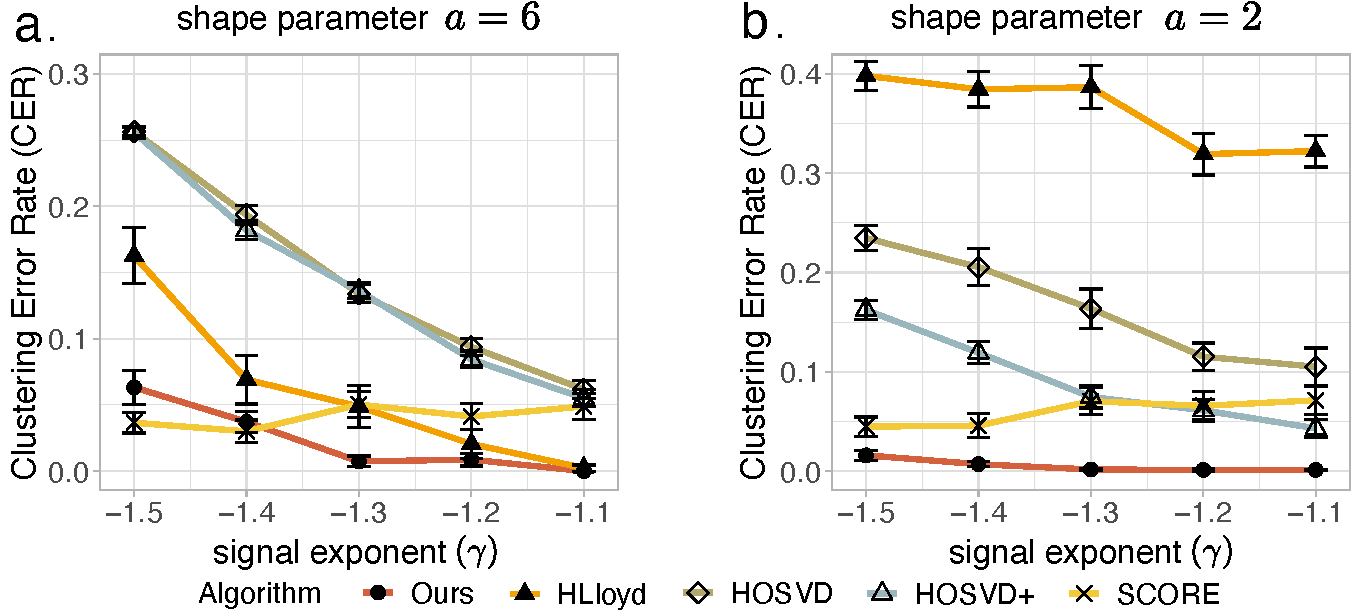
\includegraphics[width=.8\columnwidth]{comp_gamma_theta3.pdf}
    \caption{CER comparison versus signal exponent (denoted $\gamma$) under (a) low (shape parameter $a = 6$)  (b) high (shape parameter $a = 2$) degree heterogeneity. We set $p = 100, r = 5, \gamma \in [-1.5, -1.1]$ under Gaussian model.}
    \label{fig:comp_gamma_theta}
\end{figure}

The last experiment investigates the effects of degree heterogeneity to clustering performance. We fix the signal exponent $\gamma = -1.2$ and vary the extent of degree heterogeneity. In this experiment, we generate $\mtheta$ from Pareto distribution prior to normalization. We vary the shape parameter $a \in [3,6]$ in the Pareto distribution to investigate a range of degree heterogeneities. Figure~\ref{fig:comp_theta} demonstrates the stability of degree-corrected algorithms (\textbf{\small dTBM}, \textbf{\small SCORE}, \textbf{\small HOSVD+}) over the entire range of degree heterogeneity under consideration. In contrast, non-degree algorithms (\textbf{\small HLloyd}, \textbf{\small HOSVD}) show poor performance with large heterogeneity, especially in Bernoulli cases. This experiment, again, highlights the benefit of addressing degree heterogeneity in higher-order clustering. 


\section{Real data applications}\label{sec:real}
\subsection{Human brain connectome data analysis}

The Human Connectome Project (HCP) aims to construct the structural and functional neural connections in human brains~\citep{van2013wu}. We preprocess the original dataset following \cite{desikan2006automated} and partition the brain into 68 regions. The cleaned dataset includes brain networks for 136 individuals. Each brain network is represented by a 68-by-68 binary symmetric matrix, where the entry with value 1 indicates the presence of connection between node pairs, while the value 0 indicates the absence. We use $\tY \in \{0,1\}^{68 \times 68 \times 136}$ to denote the binary tensor. Individual attributes such as gender and sex are recorded.

We apply our generalized algorithm to the HCP data with the numbers of clusters on three modes $r_1 = r_2 = 4$ and $r_3 = 3$. The selection of $r_1$ and $r_2$ follows the human brain anatomy and the symmetry in the brain network, and the $r_3$ is specified following previous analysis~\citep{hu2021generalized}. Because of the symmetry in the data, the estimated brain node clustering results are the same on the first and second modes. Figure~\ref{fig:cluster_brain} shows that brain connection exhibits a strong spatial separation structure. Specifically, the first cluster, named \emph{L.Hemis}, involves all the nodes in the left hemisphere. The nodes in the right hemisphere are further separated into three clusters led by the middle-part tissues in Temporal and Parietal lobes (\emph{R.Temporal}), the back-part tissues in Occipital lobe (\emph{R.Occipital}), and the front-part tissues in Frontal and Parietal lobes (\emph{R.Supra}). This clustering result is reasonable since the left and right hemispheres often play different roles in human brains. 


\begin{figure}[htb]
    \centering
    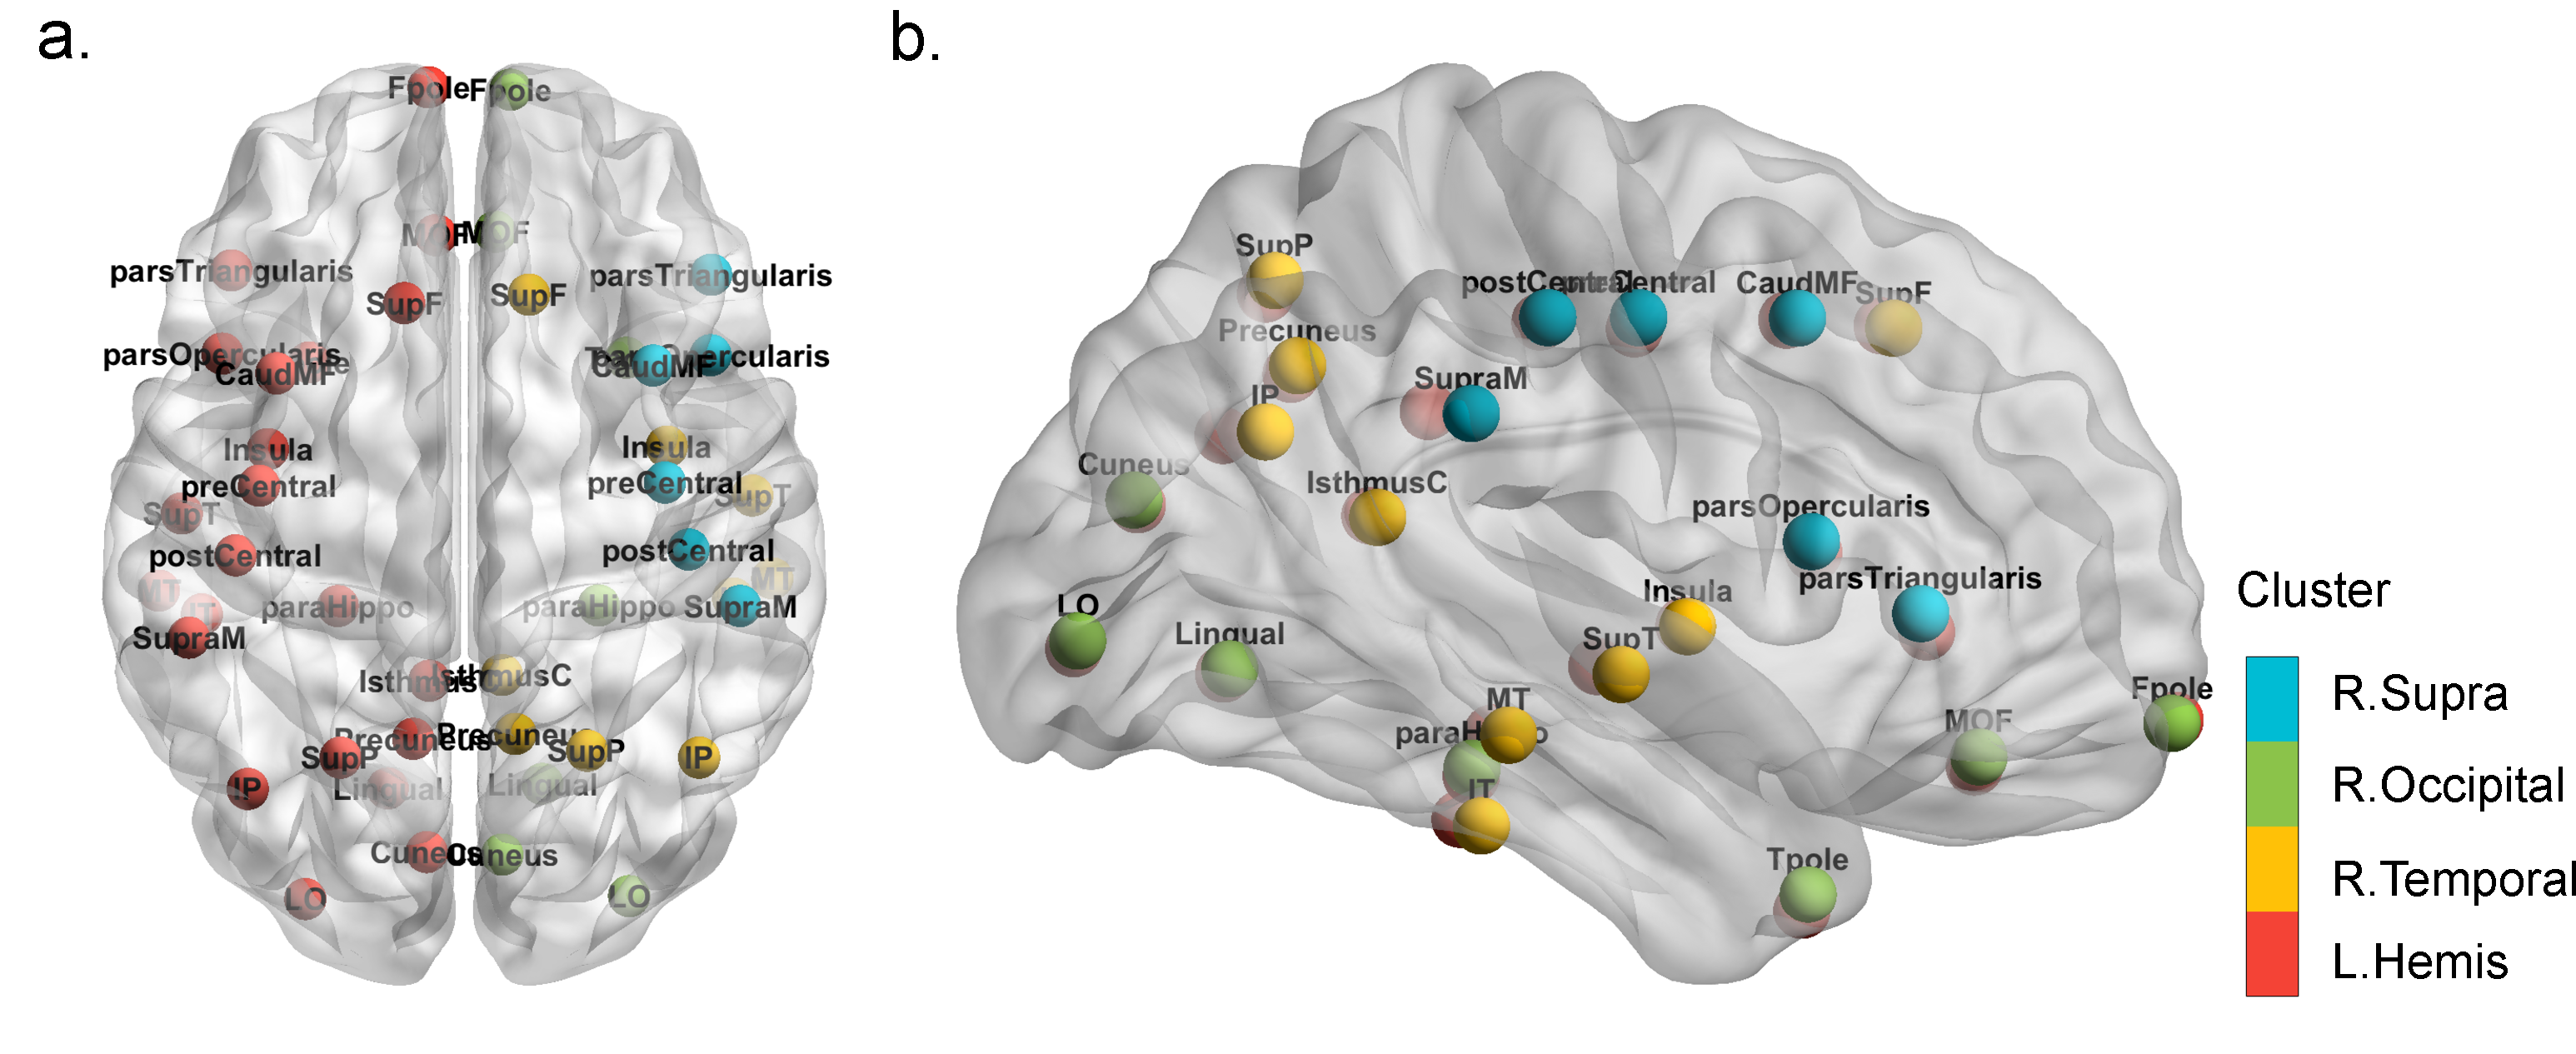
\includegraphics[width = .8\columnwidth]{brain_node_cluster.pdf}
    \caption{Illustration of brain node clustering results for HCP data with (a) top and (b) side views. }
    \label{fig:cluster_brain}
\end{figure}

\begin{figure*}[htb]
    \centering
    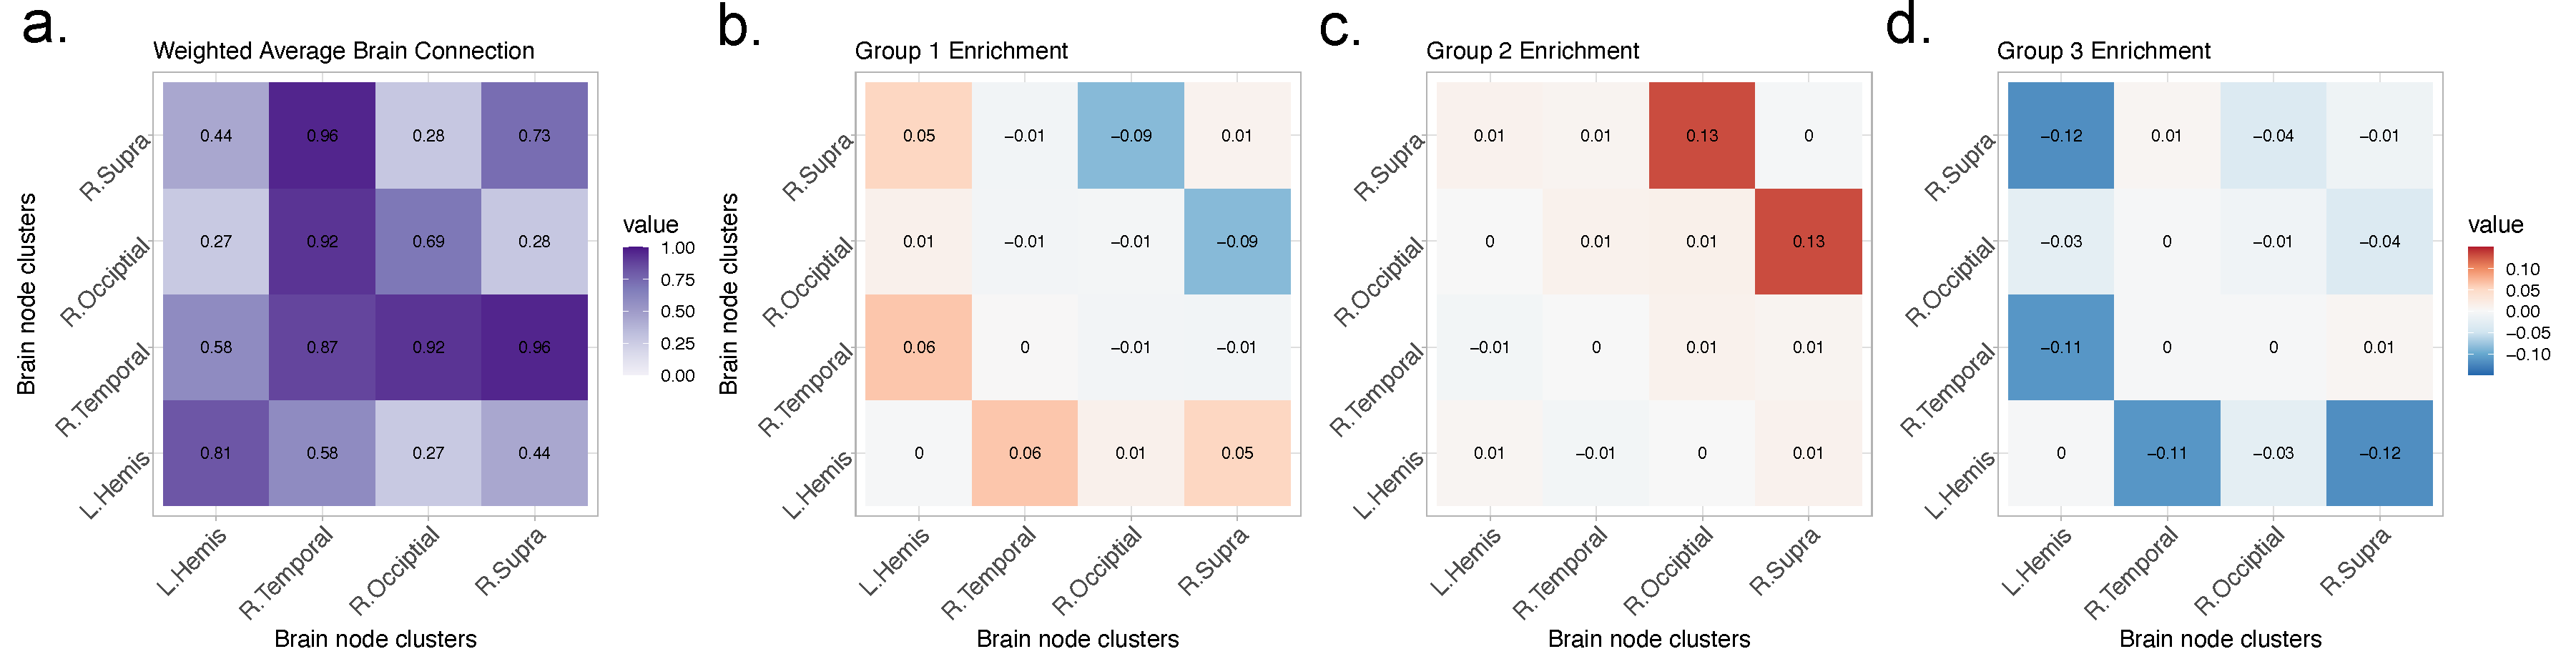
\includegraphics[width = 1\textwidth]{est_S_anno.pdf}
    \caption{Mode 3 slices of estimated core tensor $\hat \tS$. (a) Average estimated slice weighted by the group size; (b)-(d) Group-specified enrichment, i.e., the difference between each slice of $\hat \tS$ and the averaged slice. }
    \label{fig:ests}
\end{figure*}

\begin{figure*}[htb]
    \centering
    \includegraphics[width = 1\textwidth]{brain_connection.pdf}
    \caption{Observed brain connections in the population and each group of individuals. (a) Average brain network; (b)-(d) Group-specified brain network enrichments in Groups 1-3. Red edges represent the positive enrichment and blue edges represent the negative enrichment.}
    \label{fig:brain_conn}
\end{figure*}

Figure~\ref{fig:ests} illustrates the estimated core tensor $\hat \tS$ with estimated clustering, and Figure~\ref{fig:brain_conn} visualizes the average brain connections and the connection enrichment in contrast to average networks in each group. In general, we find that the inner-hemisphere connection has stronger connection compared to inter-hemisphere connections (Figure~\ref{fig:ests}a). Also, the back and front parts (\emph{R.Occipital}, \emph{R.Supra}) are shown to have more interactions with temporal tissues than inner-cluster connections. In addition, the group 1 with 54\% females shows an enrichment on the inter-hemisphere connections (Figure~\ref{fig:ests}b), while group 4 with only 36\% females exhibits a reduction (Figure~\ref{fig:ests}d). This result agrees with previous findings in \cite{hu2021generalized}. The enrichment on the back-front connection is also recognized in group~3 (Figure~\ref{fig:ests}c). The interpretive patterns in our results demonstrate the usefulness of our clustering methods in the human brain connectome data application. 


\subsection{Peru Legislation data analysis}

We also apply our method to the legislation networks in the Congress of the Republic of Peru \citep{lee2017time}. Because of the frequent political power shifts in the Peruvian Congress during 2006-2011, we choose to focus on the data for the first half of 2006-2007 year. The dataset records the co-sponsorship of 116 legislators from top 5 parties and 802 bill proposals. We reconstruct legislation network as an order-3 binary tensor $\tY \in \{0,1\}^{116 \times 116 \times 116}$, where $\tY_{ijk} = 1$ if the legislators $(i,j,k)$ have sponsored the same bill, and $\tY_{ijk} = 0$ otherwise. The true party affiliations of legislators are provided and serve as the ground truth. We apply various higher-order clustering methods to $\tY$ with $r = 5$. Table~\ref{tab:peru} shows that our \textbf{\small dTBM} achieves the best performance compared to others. The second best method is the two-stage algorithm \textbf{\small HLloyd}, followed by the spectral methods \textbf{\small SCORE} and \textbf{\small HOSVD+}. This result is consistent with our simulations under strong signal and moderate degree heterogeneity. The comparison suggests that our method \textbf{\small dTBM} is more appealing in real-world applications.

\begin{table}[ht]
    \centering
    \begin{tabular}{c |c  c cc c}
    \hline
        Method & \textbf{\small dTBM} 
        &\textbf{\small HOSVD}
        &\textbf{\small HOSVD+} & \textbf{\small HLloyd} &  \textbf{\small SCORE}\\
         CER & \textbf{0.116}
         &  0.22 
         &0.213 & 0.149 &0.199\\
         \hline
    \end{tabular}
    \caption{Clustering errors (measured by CER) for various methods in the analysis of Peru Legislation dataset.}
    \label{tab:peru}
\end{table}



\section{Proof Sketches}\label{sec:mainproof}

In this section, we provide the proof sketches for the main Theorems~\ref{thm:initial}-\ref{thm:refinement}. Detail proofs and extra theoretical results are provided in Appendix.


\subsection{Proof sketch of Theorem~\ref{thm:initial}}
The proof of Theorem~\ref{thm:initial} is inspired by the proof idea of \citet[Lemma 1]{gao2018community}. The extra difficulties are the angle gap characterization and multilinear algebra property in tensors; we address both challenges in our proof. Specifically, we control the misclustering error by the estimation error of $\hat \tX$ calculated in Step 2 of Sub-algorithm~\hyperref[alg:main]{1}.  We prove the following inequality
\begin{equation}\label{eq:proof_4}
    \ell(z^{(0)},z) \lesssim \frac{1}{p}\min_{\pi \in \Pi} \sum_{i: z^{(0)}(i) \neq \pi(z(i))} \theta(i)^2 \lesssim \frac{\sigma^2 r^{K-1}}{ \Delta_{\min}^2 p^K} \onormSize{}{\hat \tX - \tX}_F^2 \lesssim \frac{r^K p^{-K/2}}{\text{SNR}},
\end{equation}
where $\tX = \bbE \tY$ is the true mean. The first inequality in~\eqref{eq:proof_4} holds with the assumption $\min_{i \in [p]} \theta(i) \geq c>0$ in Theorem~\ref{thm:initial}. The second inequality relies on an important conclusion that the angle gap of mean tensor $\tX$ is lower bounded by that of core tensor $\tS$, i.e., the minimal angle gap $\Delta_{\min}$ defined in Assumption~\ref{assmp:min_gap}. Let $\ma^{s} \coloneqq \ma/\onorm{\ma}$ denote the normalized vector with the convention that $\ma^s = 0$ if $\ma = 0$. We want to show that
\begin{equation}\label{eq:proof_4_gap}
\min_{z(i) \neq z(j)} \onormSize{}{[\mX_{i:}]^s - [\mX_{j:}]^s} \gtrsim \Delta_{\min},
\end{equation}
where $\mX = \mat(\tX)$. The most challenging part in the proof of Theorem~\ref{thm:initial} lies in the derivation of inequality~\eqref{eq:proof_4_gap}, in which the proof of \cite{gao2018community} is no longer applicable due to different angle gap assumption in our dTBM. We develop the extra padding technique in Lemma~\ref{lem:pad} and balance assumption~\eqref{eq:degree} to derive~\eqref{eq:proof_4_gap}. Last, we finish the proof of Theorem~\ref{thm:initial} by showing the third inequality of~\eqref{eq:proof_4} using \citet[Proposition 1]{han2020exact}. 


\subsection{Proof sketch of Theorem 5}
The proof of Theorem~\ref{thm:refinement} is inspired by the proof idea of \citet[Theorem 2]{han2020exact}. We develop extra polar-coordinate based techniques with angle gap characterization to address the nuisance degree heterogeneity. We introduce an intermediate quantity called misclustering loss
\begin{equation}
     L^{(t)} = \frac{1}{p}  \sum_{i \in [p]} \theta(i) \sum_{b \in [r]}  \ind \offf{ z^{(t)}(i) = b } \onorm{ \off{ \mS_{ z(i):}  }^s - \off{ \mS_{b:}  }^s  }^2,
\end{equation}
where the superscript $\cdot^{s}$ denotes the normalized vector; i.e., $\ma^s:=\ma/\onorm{\ma}$ if $\ma\neq 0$ and $\ma^{s}=0$ if $\ma=0$ for any vector $\ma$. We show that $L^{(t)}$ provides an upper bound for the misclassification error of interest via the inequality $\ell^{(t)}\leq {L^{(t)}\over \Delta^2_{\min}}$. Therefore, it suffices to control $L^{(t)}$. Further, we introduce the oracle estimators for core tensor under the true cluster assignment via 
\begin{equation}
    \tilde \tS = \tY \times_1 \mW^T \times_2 \cdots \times_K \mW^T, 
\end{equation}
where $\mW = \mM \of{ \text{diag}(\mone_{p}^T \mM) }^{-1}$ is the weighted true membership matrix. Let $ \mV = \mW^{\otimes (K-1)}$ denote the Kronecker product of $(K-1)$ copies of $\mW$ matrices, and we define the $t$-th iteration quantities $\mW^{(t)}, \mV^{(t)}$ corresponding to $\mM^{(t)}$ (or equivalently $z^{(t)}$). To evaluate $L^{(t+1)}$, we prove the bound
\begin{equation}\label{eq:proof_5_event}
    \ind \offf{ z^{(t+1)}(i) = b } = \ind \offf{       \onormSize{}{ [ \mY_{i:} \mV^{(t)}  ]^s - [\mS_{b:}^{(t)}]^s }^2 \leq \onormSize{}{ [ \mY_{i:} \mV^{(t)}  ]^s - [\mS_{z(i):}^{(t)}]^s }^2} \leq A_{ib} + B_{ib},
\end{equation}
where $\mY = \mat(\tY)$, $ \mS = \mat(\tS)$, $\mS^{(t)} = \mat(\tS^{(t)})$ and
\begin{align}
        A_{ib} &= \ind \offf{\ang{ \mE_{i:} \mV, \off{  \tilde \mS_{z(i):} }^s - \off{  \tilde \mS_{b:} }^s } \lesssim -  \onorm{ \off{ \mS_{z(i):}  }^s - \off{ \mS_{b:}  }^s  }^2 },\\
        B_{ib} &= \ind \offf{\onorm{ \off{ \mS_{z(i):}  }^s - \off{ \mS_{b:}  }^s  }^2 \lesssim F_{ib}^{(t)} + G_{ib}^{(t)} + H_{ib}^{(t)} }.
\end{align}
The terms $F_{ib}^{(t)}, G_{ib}^{(t)}, H_{ib}^{(t)}$ are controlled by $z^{(t)}, \tS^{(t)}$; see the detailed definitions in \eqref{eq:f}, \eqref{eq:g}, \eqref{eq:h}. Note that the event $A_{ib}$ only involves the oracle estimator independent of $t$, while all the terms related to the $t$-th iteration are in $B_{ib}$. Thus, the inequality~\eqref{eq:proof_5_event} decomposes the misclustering loss in the $(t+1)$-th iteration into the oracle loss and the loss in $t$-th iteration. This decomposition leads to the separation of statistical error and computational error in the final upper bound of Theorem~\ref{thm:refinement}.

Specifically, we prove the contraction inequality
\begin{equation}\label{eq:proof_5_ineq}
    L^{(t+1)} \leq M \xi + \rho L^{(t)}, \quad \xi = \frac{1}{p}  \sum_{i \in [p]} \theta(i) \sum_{b \in [r]}  A_{ib} \onorm{ \off{ \mS_{ z(i):}  }^s - \off{ \mS_{b:}  }^s  }^2,
\end{equation}
where $M$ is a positive constant, $\rho \in (0,1)$ is the contraction parameter, and we call $\xi$ the oracle loss. Controlling the probability of event $B_{ib}$ and obtaining the $\rho L^{(t)}$ term in the right hand side of~\eqref{eq:proof_5_ineq} are the most challenging parts in the proof of Theorem~\ref{thm:refinement}. Note that the true and estimated core tensors are involved via their normalized rows such as $\mS_{a:}^s, \tilde \mS_{a:}^s, [\mS^{(t)}_{a:}]^s$. The Cartesian coordinate based analysis in \cite{han2020exact} is no longer applicable in our case. Instead, we use the polar-coordinate based analysis and the geometry property of trigonometric functions to derive the high probability upper bounds for $F_{ib}^{(t)}, G_{ib}^{(t)}, H_{ib}^{(t)}$. 

Further, by sub-Gaussian concentration, we prove the high probability upper bound for oracle loss
\begin{equation}\label{eq:proof_5_xi}
    \xi  \lesssim \exp\of{- \frac{p^{K-1}\text{SNR}}{r^{K-1}}}.
\end{equation}
Combining the decomposition~\eqref{eq:proof_5_ineq} and the oracle bound~\eqref{eq:proof_5_xi}, we finish the proof of Theorem~\ref{thm:refinement}.


\section*{Acknowledgments}
This research is supported in part by NSF grants DMS-1915978, DMS-2023239, EF-2133740, and funding from the Wisconsin Alumni Research foundation. We thank Zheng Tracy Ke, Rungang Han, Yuetian Luo for helpful discussions and for sharing software packages. 

\bibliographystyle{apalike}
\bibliography{tensor_wang}



\newpage
\appendix


We provide the proofs for all the theorems in our main paper. In each sub-section, we first show the proof of main theorem and then collect the useful lemmas in the end.

\section*{Notation}
Before the proofs, we first introduce the notation used throughout the appendix and the generalized dTBM without symmetric assumptions. The parameter space and minimal gap assumption are also extended for the generalized dTBM. 

{\bf Preliminaries.}
\begin{enumerate}[wide]
    \item For mode $ k \in [K]$, denote the mode-$k$ tensor matricizations by
    \begin{equation}
        \mY_k = \mat_k \of{ \tY }, \quad \mS_k = \mat_k \of{\tS}, \quad \mE_k = \mat_k \of{ \tE}, \quad \mX_k = \mat_k \of{\tX}.
    \end{equation}
    \item For a vector $\ma$, let $\ma^{s} \coloneqq \ma/\onorm{\ma}$ denote the normalized vector. We make the convention that $\ma^s = {\bf 0}$ if $\ma = {\bf 0}$. 
    \item For a matrix $\mA \in \bbR^{n \times m} $, let $\mA^{\otimes K}:=\mA\otimes \cdots \otimes \mA\in \bbR^{n^K \times m^K}$ denote the Kronecker product of $K$ copies of matrices $\mA $.
    \item For a matrix $\mA$, let $\onormSize{}{\mA}_\sigma$ denote the spectral norm of matrix $\mA$, which is equal to the maximal singular value of $\mA$; let $\lambda_k(\mA)$ denote the $k$-th largest singular value of $\mA$; let $\onormSize{}{\mA}_F$ denote the Frobenius norm of matrix $\mA$.
    \item For two sequence $a$ and $b$, let $a \asymp b$ if there exist two positive constants $c, C$ such that $cb \leq a\leq Cb$. 
\end{enumerate}


{\bf Model extension to generalized dTBM.} 
 
 The general order-$K$ $(p_1, \ldots, p_K)$-dimensional dTBM model with $r_k$ communities and degree heterogeneity $\mtheta_k = \entry{\theta_k(i)} \in \bbR_+^{p_k}$ is represented by
\begin{equation}\label{eq:general_dtbm}
    \tY = \tX+ \tE,\quad \text{where}\quad \tX=\tS \times_1 \mTheta_1 \mM_1 \times_2 \cdots \times_K \mTheta_K \mM_K,
\end{equation}
where $\tY \in \bbR^{p_1 \times \cdots \times p_K}$ is the data tensor, $\tX\in \mathbb{R}^{p_1\times \cdots \times p_K}$ is the mean tensor, $\tS \in \bbR^{r_1 \times \cdots \times r_K}$ is the core tensor, $\tE \in \bbR^{p_1 \times \cdots \times p_K}$ is the noise tensor consisting of independent zero-mean sub-Gaussian entries with variance bounded by $\sigma^2$, $\mTheta_k = \text{diag}(\mtheta_k)$, and $\mM_k\in \{0,1\}^{p_k \times r_k}$ is the membership matrix corresponding to the assignment $z_k: [p_k] \mapsto [r_k]$, for all $k \in [K]$. 

For ease of notation, we use $\{z_k\}$ to denote the collection $\{z_k\}_{k=1}^K$, and $\{\mtheta_k\}$ to denote the collection $\{\mtheta_k\}_{k=1}^K$. Correspondingly, we consider the parameter space for the triplet $\of{\{z_k\}, \tS, \{\mtheta_k\}}$,

\begin{align}
 \tP(\{r_k\}) = \Bigg\{ &\of{\{z_k\}, \tS, \{\mtheta_k\}}:\\
   & \mtheta_k \in\mathbb{R}^p_{+}, {c_1 p_k\over r_k} |z_k^{-1}(a)| \leq {c_2 p_k\over r_k}, c_3 \leq  \onorm{\mS_{k,a:}} \leq c_4 ,\onormSize{}{\mtheta_{k,z_k^{-1}(a)}}_1=|z_k^{-1}(a)|, a \in [r_k], k\in[K]\Bigg\}. \label{eq:general_family}
\end{align}


We call the degree heterogeneity $\{\mtheta_k\}$ is balanced if for all $k \in [K]$,
\begin{equation}\label{eq:general_balanced}
    {\min_{a\in[r]} \onormSize{}{\mtheta_{k, z_k^{-1}(a)}}=\left(1+o(1)\right)\max_{a\in[r]}\onormSize{}{\mtheta_{k,z_k^{-1}(a)}}}.
\end{equation}

We also consider the generalized Assumption~\ref{assmp:min_gap} on angle gap.
\begin{assumption}[Generalized angle gap]\label{assmp:general_minimal_gap} Recall $\mS_k=\mat_k(\tS)$. We assume the minimal gap between normalized rows of $\mS_k$ is bounded away from zero for all $k\in[K]$; i.e.,
\begin{equation}
     \Delta_{\min} \coloneqq \min_{k \in [K]} \min_{a \neq b \in [r_k]} \onorm{ \mS_{k,a:}^s - \mS_{k, b:}^s } > 0.
\end{equation}
\end{assumption}
Similarly, let $\text{SNR} = \Delta_{\min}^2/\sigma^2$ with the generalized minimal gap $\Delta_{\min}^2$ defined in Assumption~\ref{assmp:general_minimal_gap}. We define the regime
\begin{equation}
    \tP(\gamma) = \tP (\{r_k\}) \cap\{\tS \text{ satisfies $\text{SNR} = p^{\gamma}$ and $p_k \asymp p, \text{for all }k \in [K]$} \}.
\end{equation}



\section*{Proof of Theorem~\ref{thm:unique}}

\begin{proof}[Proof of Theorem~\ref{thm:unique}] 

To study the identifiability, we consider the noiseless model with $\tE = 0$. Assume there exist two parameterizations satisfying
\begin{equation}\label{eq:another}
    \tX=\tS\times_1\Theta_1 \mM_1 \times_2 \cdots \times_K \Theta_K \mM'_K=\tS'\times_1\Theta'_1 \mM'_1 \times_2 \cdots \times_K \Theta'_K \mM'_K,
\end{equation}
where $\of{ \{z_k\}, \tS, \{ \mtheta_k \} } \in \tP(\{r_k\})$ and $\of{ \{z'_k\}, \tS', \{ \mtheta'_k \} } \in \tP(\{r_k'\})$ are two sets of parameters. We prove the sufficient and necessary conditions separately.

\begin{enumerate}[wide]
    \item[$(\Leftarrow)$] For the necessity, it suffices to construct two distinct parameters up to cluster label permutation, if the model~\eqref{eq:general_dtbm} violates Assumption~\ref{assmp:general_minimal_gap}. Without loss of generality, we assume $\onorm{ \mS_{1,1:}^s - \mS_{1,2:}^s } = 0$.

 If $\mS_{1,1:}$ is a zero vector, construct $\mtheta_1'$ such that $\mtheta'_{1,z_1^{-1}(1)} \neq \mtheta_{1,z_1^{-1}(1)}$. Let $\{z'_k\} = \{z_k\}$, $\tS' = \tS$, and $\mtheta'_k = \mtheta_k$ for all $k = 2, \ldots, K$. Then the triplet $\of{ \{z'_k\}, \tS', \{ \mtheta'_k \} }$ is distinct from $\of{ \{z_k\}, \tS, \{ \mtheta_k \} }$ up to label permutation. Similar conclusion holds when $\mS_{1,2:}$ is a zero vector. 

If neither $\mS_{1,1:}$ nor $\mS_{1,2:}$ is a zero vector, there exists a positive constant $c$ such that $\mS_{1,1:} = c \mS_{1,2:}$. Thus, there exists a core tensor $\tS_0 \in \bbR^{r_1 -1 \times \cdots \times r_K}$ such that 
\begin{equation}
    \tS = \tS_0 \times_1 \mC \mR, \quad \text{where} \quad \mC = \text{diag}(1, c, 1,...,1) \in \bbR^{r_1 \times r_1}, \quad \mR = \begin{pmatrix}
    1& 0\\
    1&0 \\
    0 & \mone_{r_1-2}
    \end{pmatrix} \in \bbR^{r_1 \times (r_1 -1)}.
\end{equation}
Let $\mD = \text{diag}(1+c, 1,...,1) \in \bbR^{r_1 -1 \times r_1 -1}$. Consider the parameterization
\begin{equation}
    \mM'_1 = \mM_1 \mR, \quad \tS' = \tS_0 \times_1 \mD, \quad \theta'_{1}(i) = \begin{cases}
    \frac{1}{1+c} \theta_{1}(i) & i \in z_{1}^{-1}(1),\\
     \frac{c}{1+c} \theta_{1}(i) & i \in z_{1}^{-1}(2),\\
     \theta_{1}(i) & \text{ otherwise},
    \end{cases}
\end{equation}
and $\mM'_k = \mM_k, \mtheta'_k = \mtheta_k$ for all $k = 2, \ldots, K$. Then we have constructed a
triplet $\of{ \{z'_k\}, \tS', \{ \mtheta'_k \} }$ that is distinct from $\of{ \{z_k\}, \tS, \{ \mtheta_k \} }$ up to label permutation. 

\item[$(\Rightarrow)$] For the sufficiency, it suffices to show that all possible triplets $\of{ \{z'_k\}, \tS', \{ \mtheta'_k \} }$ are identical to $\of{ \{z_k\}, \tS, \{ \mtheta_k \} }$ up to label permutation if the model~\eqref{eq:general_dtbm} satisfies Assumption~\eqref{assmp:general_minimal_gap}. We show the uniqueness of the three parameters, $\{\mM_k\}, \{\tS\}, \{\mtheta_k\}$ separately.

First, we show the uniqueness of $\mM_k$ for all $k \in [K]$. Without loss of generality, we consider $k=1$ and show the first mode membership matrix; i.e., $\mM'_1 = \mM_1\mP_1$ where $\mP_1$ is a permutation matrix. The conclusion for $k\geq 2$ can be showed similarly and thus omitted. 

Consider an arbitrary node pair $(i,j)$. If $z_1(i) = z_1(j)$, then we have $\onormSize{}{\mX_{1, z_1(i):}^s - \mX_{1, z_1(j):}^s } = 0$ and thus $\onormSize{}{ (\mS')_{1, z'_1(i):}^{s} - (\mS')_{1, z'_1(j):}^{s} } = 0$ by Lemma~\ref{lem:angle}. Then, by Assumption~\eqref{assmp:general_minimal_gap}, we have $z'_1(i) = z'_1(j)$. Conversely, if $z_1(i) \neq z_1(j)$, then we have $ \onorm{\mX_{1,i:}^s - \mX_{1,j:}^s} \neq 0$ and thus $\onorm{ (\mS')_{1, z'_1(i):}^{s} - (\mS')_{1, z'_1(j):}^{s} } \neq 0$ by Lemma~\ref{lem:angle}. Hence, we have $z'_1(i) \neq z'_1(j)$. Therefore, we have proven that $z'_1$ is identical $z_i$ up to label permutation.

Next, we show the uniqueness of $\mtheta_k$ for all $k \in [K]$ provided that $z_k = z_k'$. Similarly, consider $k=1$ only, and omit the procedure for $k\geq 2$. 

Consider an arbitrary $j \in [p_1]$ such that $z_1(j) = a$. Then for all the nodes $i \in  z_1^{-1}(a)$ in the same cluster of $j$, we have 
\begin{equation}
    \frac{\mX_{1,z_1(i):}}{\mX_{1,z_1(j):}} = \frac{\mX'_{1,z_1(i):}}{\mX'_{1,z_1(j):}}, \text{ which implies }  \frac{\theta_1(j)}{\theta_1(i)} = \frac{\theta'_1(j)}{\theta'_1(i)}.\label{eq:theta_uniq}
\end{equation}
Let $\theta'_1(j) = c\theta_1(j)$ for some positive constant $c$. By equation~\eqref{eq:theta_uniq}, we have $\theta'_1(i) = c \theta_1(i)$ for all $ i \in  z_1^{-1}(a)$. By the constraint $(\{z_k\}, \tS', \{\mtheta'_k\}) \in \tP(\{r_k\})$, we have 
\begin{equation}
    \sum_{j \in z_1^{-1}(a)} \theta'_1(j) = c \sum_{j \in z_1^{-1}(a)} \theta_1(j) = 1,
\end{equation}
which implies $c = 1$. Hence, we have proven $\mtheta_1 = \mtheta'_1$ provided that $z_1 = z'_1$.

Last, we show the uniqueness of $\tS$; i.e., $\tS'=\tS\times_1 \mP^{-1}_1\times_2\cdots \times_K \mP^{-1}_K$, where $\mP_k$'s are permutation matrices for all $k\in[K]$.  Provided $z'_k = z_k, \mtheta'_k = \mtheta_k$, we have $\mM'_k = \mM_k \mP_k$ and $\mTheta'_k = \mTheta_k$ for all $k \in [K]$. 

Let $\mD_k = \off{ (\mTheta'_k \mM'_k)^T (\mTheta'_k \mM'_k) }^{-1} (\mTheta'_k \mM'_k)^T, k \in [K]$. By the parameterization~\eqref{eq:another}, we have 
\begin{align}
    \tS' &= \tX \times_1 \mD_1 \times_2 \cdots \times_K \mD_K \\
    &= \tS \times_1 \mD_1 \mTheta_1 \mM_1 \times_1 \cdots \times_K \mD_K \mTheta_K \mM_K \\
    &= \tS \times_1 \mP^{-1}_1 \times_2 \cdots \times_K \mP^{-1}_K.
\end{align}


\end{enumerate}

Therefore, we finish the proof of Theorem~\ref{thm:unique}.
\end{proof}


{\bf Useful Lemma for the Proof of Theorem~\ref{thm:unique}} 

\begin{lem}[Motivation of angle-based clustering]\label{lem:angle} Consider the signal tensor $\tX$ in the generalized dTBM~\eqref{eq:general_dtbm} with $(\{z_k\},\tS,\{\mtheta_k\})\in \tP(\{r_k\})$ and $r_k \geq 2$. Then, for any $k \in [K]$ and index pair $(i,j)\in[p_k]^2$, we have 
\begin{equation}
    \onorm{ \mS_{k,z_k(i):}^s -  \mS_{k,z_k(j):}^s } = 0 \quad \text{if and only if} \quad \onorm{  \mX_{k, z_k(i):}^s -  \mX_{k,z_k(j):}^s } = 0.
\end{equation}
\end{lem}

\begin{proof}[Proof of Lemma~\ref{lem:angle}] Without loss of generality, we prove $k = 1$ only and drop the subscript $k$ in $\mX_k, \mS_k$ for notational convenience. 
By tensor matricization, we have
\begin{equation}
    \mX_{j:} = \theta_1(j) \mS_{z_1(j):} \off{\mTheta_2 \mM_2 \otimes \cdots \otimes \mTheta_K \mM_K}^T.
\end{equation}     
Let $\tilde \mM = \mTheta_2 \mM_2 \otimes \cdots \otimes \mTheta_K \mM_K$. Notice that for two vectors $\ma, \mb$ and two positive constants $c_1, c_2 >0$, we have
\begin{equation}
\onorm{\ma^s - \mb^s} = \onorm{(c_1 \ma)^s - (c_2\mb)^s}.
\end{equation}
Thus it suffices to show the following statement holds for any index pair $(i,j)\in[p_1]^2$,
\begin{equation}
\onorm{ \mS_{z_1(i):}^s - \mS_{z_1(j):}^s} = 0 \quad \text{if and only if} \quad \onorm{ \off{\mS_{z_1(i):} \tilde \mM^T }^s - \off{\mS_{z_1(j):}\tilde \mM^T}^s} = 0.
\end{equation}
\begin{enumerate}[wide]
    \item[$(\Leftarrow)$] Suppose $\onorm{ \off{\mS_{z_1(i):} \tilde \mM^T }^s - \off{\mS_{z_1(j):}\tilde \mM^T}^s} = 0$. There exists a positive constant $c$ such that $\mS_{z_1(i):} \tilde \mM^T= c \mS_{z_1(j):} \tilde \mM^T$. Note that
\begin{equation}
    \mS_{z_1(i):} = \mS_{z_1(i):} \tilde \mM^T \off{ \tilde \mM \of{ \tilde \mM^T  \tilde \mM}^{-1}},
\end{equation}
where $ \tilde \mM^T  \tilde \mM$ is an invertiable diagonal matrix with positive diagonal elements. Thus, we have $ \mS_{z_1(i):} = c  \mS_{z_1(j):}$, which implies $ \onorm{  \mS_{z_1(i):}^s -  \mS_{z_1(j):}^s } = 0 $.

\item[$(\Rightarrow)$] Suppose $ \onorm{ \mS_{z_1(i):}^s - \mS_{z_1(j):}^s } = 0 $. There exists a positive constant $c$ such that $\mS_{z_1(i):} = c \mS_{z_1(j):}$, and thus $\mS_{z_1(i):} \tilde \mM^T = c \mS_{z_1(j):} \tilde \mM^T$, which implies $\onorm{\left[\mS_{z_1(i):} \tilde \mM^T\right]^s- \left[\mS_{z_1(j):} \tilde \mM^T\right]^s}=0$.
\end{enumerate}
Therefore, we finish the proof of Lemma~\ref{lem:angle}.
\end{proof}



\section*{Proof of Theorem~\ref{thm:stats}}

\begin{proof}[Proof of Theorem~\ref{thm:stats}]
We will prove a more general conclusion than the main paper by allowing growing $r_k$'s. Consider the generalized dTBM~\eqref{eq:general_dtbm} in the special case that $p_k = p$ and $r_k = r$ for all $ k\in [K]$. Specifically, we will show that, under 
the assumptions $K\geq 1$, $r\lesssim p^{1/3}$ and SNR condition
\[
{\Delta^2_{\min}\over \sigma^2}\lesssim {r^{K-1}\over p^{K-1}},\quad \text{or equivalently}, \quad \gamma\leq -(K-1)(1+\log_p r),
\]
 the desired conclusion in Theorem~\ref{thm:stats} holds; i.e, for all $k \in [K]$, every estimator $\hat z_{k,\text{stat}}$ obeys
\begin{equation}\label{eq:max}
    \sup_{(\{z_k\}, \tS, \{\mtheta_k\}) \in \tP(\gamma)} \bbE \left[ p\ell(\hat z_{k,\text{stat}}, z_k) \right]\geq 1.
\end{equation}

Since the inequality~\eqref{eq:max} is a minimax lower bound, it suffices to show the inequality holds for a particular $(\{z_k\}, \tS, \{\mtheta_k\}) \in \tP(\gamma)$. Specifically, we consider the estimation problem based on a particular parameter point $(\{z_k\}, \tS, \{\mtheta_k\})$ with the following three properties:
\begin{equation}\label{eq:construction}
    \text{(i)}\  \theta_k(i)=1 \text{ for all }i\in[p]; \quad  \text{(ii)}\ 
    \Delta_{\min}\lesssim  \left({p\over r}\right)^{-\frac{K-1}{2}}\sigma; \quad  \text{(iii)}\ |z^{-1}_k(a)|={p \over r} \in \mathbb{Z}_+ \text{ for all }a\in[r],
\end{equation}
for all $k \in [K]$.
Furthermore, we define a subset of indices $T_k \subset [p_k], k \in [K]$ in order to avoid the complication of label permutation. Based on \citet[Proof of Theorem 6]{han2020exact}, we consider the minimax rate over the restricted family of $\hat z_k$'s for which the following three conditions are satisfied:
\begin{equation}
    \text{(iv)}\ \hat z_k(i)=z_k(i) \text{ for all }i\in T_k; \quad \text{(v)} \ |T^c_k|\asymp {p\over r}; \quad \text{(vi)}\ \min_{\pi\in \Pi}\sum_{i\in[p]}\ind\{\hat z_k(i) \neq \pi\circ z_k (i)\} = \sum_{i\in[p]}\ind\{\hat z_k(i) \neq  z_k (i)\},
\end{equation}
\normalsize
for all $k \in [K]$.
The construction of $T$ is precisely the same as \citet[Proof of Theorem 6]{han2020exact}. 
Then, following the proof of~\citet[Theorem 2]{gao2018community}, for all $k \in [K]$, we have
\begin{equation}\label{eq:minimax}
\inf_{\hat z_k}\sup_{z_k}\bbE \ell(\hat z_k, z_k) \gtrsim {1\over r^3 |T^c_k|}\sum_{i\in T^c_k}\inf_{\hat z_k}\left\{\bbP[\hat z_k(i)=2|z_k(i)=1] + \bbP[\hat z_k(i)=1|z_k(i)=2] \right\},
\end{equation}
where $\hat z_k$ and $z_k$ on the left hand side denote the generic clustering functions in $\tP(\gamma)$, $z_k$ on the right hand side denotes a particular parameter satisfying properties (i)-(vi), and the infimum on the right hand side is taken over the restricted family of $\hat z$ satisfying (iv)-(vi). Here, the factor $r^3=r\cdot r^2$ in~\eqref{eq:minimax} comes from two sources: $r^2\asymp {r\choose 2}$ comes from the multiple testing burden for all pairwise comparisons among $r$ clusters; and another $r$ comes from the number of elements $|T^c_k|\asymp p/r$ to be clustered. 

Next, we need to find the lower bound of the rightmost side in~\eqref{eq:minimax}. For simplicity, we show the bound for the mode-1 case $k = 1$ only. We drop the subscripts $1$ in $z_1, T_1, \mS_1, \mtheta_1$ and omit the repeated procedures for the cases of $k = 2,\ldots, K$. 

We consider the hypothesis test based on model~\eqref{eq:general_dtbm}. First, we reparameterize the model under the construction~\eqref{eq:construction}
\begin{equation}
    \mx_a = \off{\mat_1 \of{ \tS\times_2 \mM_2\times_3\cdots \times_K \mM_K  }}_{a:}, \quad \text{for all} \ a \in [r],
\end{equation}
where $\mx_a$'s are centroids in $\bbR^{p^{K-1}}$. Without loss of generality, we consider the lower bound for the summand in~\eqref{eq:minimax} for $i=1$. The analysis for other $i\in T^c$ are similar. For notational simplicity, we suppress the subscript $i$ and write $\my, \theta, z$ in place of $\my_1, \theta_1$ and $z(1)$, respectively. The equivalent vector problem for assessing the summand in~\eqref{eq:minimax} is
\begin{equation}\label{eq:z}
\my=\theta\mx_{z}+\me,
\end{equation}
where $\theta\in\bbR_{+}$ and $z\in \{1,2\}$ are unknown parameters, $\mx_1,\mx_2\in\bbR^{p^{K-1}}$ are given centroids, and $\me\in\bbR^{p^{K-1}}$ consists of i.i.d.\ $N(0,\sigma^2)$ entries.  Then, we consider the hypothesis testing under the model~\eqref{eq:z}:
\begin{equation}\label{eq:test}
H_0\colon z=1, \quad \text{v.s.}\quad H_\alpha\colon z=2.
\end{equation}
Note that the profile log-likelihood with respect to $z$ is
\[
\tL(z,  \theta(z);\my)\propto - \inf_{\theta>0}\onormSize{}{\my- \theta\mx_{z}}^2 \propto  \cos^2(\my, \mx_{z}) \ind\{ \langle \my,\mx_{z}\rangle  >0 \}, 
\]
and the MLE's of $\theta$ and $z$ are
\begin{equation}\label{eq:MLE}
    \hat \theta_{\text{MLE}}= \hat \theta(\hat z_{\text{MLE}})={\langle \my,\mx_{\hat z_{\text{MLE}}}\rangle \over \onorm{\mx_{\hat z_{\text{MLE}}}}^2}\vee 0 , \quad 
\hat z_{\text{MLE}}= \argmax_{a\in\{1,2\}} \offf{\cos(\my,\ \mx_a)\vee 0}. 
\end{equation}

Then, the decision rule $\hat z_{\text{MLE}} \in\{1,2\}$ based on profile log-likelihood ratio is defined as
\begin{equation}\label{eq:ratio}
\hat z_{\text{MLE}}=
\begin{cases}
1 & \text{if }\cos(\my,\mx_1)\geq  \cos(\my,\mx_2) \text{ and }\langle \my,\mx_1\rangle > 0, \\
2 & \text{if }\cos(\my,\mx_1)<\cos(\my,\mx_2) \text{ and }\langle \my,\mx_2\rangle > 0,\\
\text{1 or 2 with equal probability} & \text{otherwise.}
\end{cases}
\end{equation}

The Neyman-Pearson Lemma implies
\begin{align}\label{eq:lower}
&\inf_{\hat z}\left\{\bbP[\hat z=2|z=1] + \bbP[\hat z=1|z=2]\right\}= \bbP[\hat z_{\text{MLE}}=1|z=2]+\bbP[\hat z_{\text{MLE}}=2|z=1].
\end{align}
By symmetric, it suffices to bound $\bbP[\hat z_{\text{MLE}}=1|z=2]$. Using~\eqref{eq:ratio}, we obtain
\begin{align}\label{eq:bound}
\bbP[\hat z_{\text{MLE}}=1|z=2]&= \bbP\left[ \cos(\theta\mx_2+\me,\mx_1)\geq  \cos(\theta\mx_2+\me, \mx_2) \text{ and } \langle \theta\mx_2+\me,\mx_1\rangle > 0  \right] \notag \\
&\stackrel{(*)}{\geq} \bbP \left[\left\langle \me, {\mx^s_1 -\mx^s_2\over\onorm{\mx^s_1- \mx^s_2}}  \right\rangle  \geq {\theta \over 2}\onormSize{}{\mx_2} \onormSize{}{\mx^s_1-\mx^s_2}\rangle\right]-\notag \\
&\hspace{1cm} \bbP\left[\langle \me, \mx^s_1\rangle \leq -{\theta \over 2}\onorm{\mx_2}\left(2-\onormSize{}{\mx^s_1-\mx^s_2}^2\right)\right]\notag \\
&\stackrel{(**)}{=}\Phi\left({\theta \over 2}\onorm{\mx_2}(2-\onormSize{}{\mx^s_1-\mx^s_2}^2) \right)-\Phi\left({\theta\over 2}\onorm{\mx_2}\onormSize{}{\mx^s_1-\mx^s_2} \right),
\end{align}
where $\Phi(\cdot)$ denotes the CDF for standard normal distribution. Here step $(*)$ is based on the inequality $\bbP(A\cup B)\geq \bbP(A)-\bbP(B^c)$ and the identity $1-\langle \mx^s_1,\mx^s_2 \rangle={1\over 2}\onorm{\mx^s_1-\mx^s_2}^2$; and step $(**)$ is based on isotropic property of i.i.d.\ Gaussian distribution
\[
\left\langle\me, {\mx^s_1-\mx^s_2\over \onorm{\mx^s_1-\mx^s_2}} \right\rangle \sim N(0, \sigma^2),\quad \langle \me, \mx^s_1 \rangle \sim N(0,\sigma^2).
\]
By construction~\eqref{eq:construction} of $(\{z_k\}, \tS, \{\mtheta_k\})$ with three properties and lower bound $\min_{a\in[r]}\onorm{\mS_{a:}}\geq c_3$ in the definition of $\tP(\gamma)$, we have $\theta^*=1$, $\onorm{\mx_2}\geq \onorm{\mS_{2:}}\min_{a\in[r]}\onorm{\mtheta_{\mz^{-1}(a)}}^{K-1} \gtrsim \left(p \over r\right)^{(K-1)/2}$. Also, note that under the construction~\eqref{eq:construction}
\begin{equation}
    \cos(\mx_1, \mx_2) = \frac{\and{\mx_1, \mx_2}}{\onorm{\mx_1} \onorm{\mx_2} } = \frac{(p/r)^{K-1} \ang{\mS_{1:}, \mS_{2:}}}{ \sqrt{(p/r)^{K-1} \onorm{\mS_{1:}}^2} \sqrt{(p/r)^{K-1} \onorm{\mS_{2:}}^2} } = \cos(\mS_{1:}, \mS_{2:}),
\end{equation}
which implies $\onormSize{}{\mx^s_1-\mx^s_2} = \onormSize{}{\mS_{1:}^s-\mS_{2:}^s} = \Delta_{\min} \leq 1$. Therefore, the equation~\eqref{eq:bound} is lower bounded by
\begin{equation}\label{eq:normal}
\bbP[\hat z_{\text{MLE}}=1|z=2] \geq \bbP\left[ \left({p\over r}\right)^{(K-1)/2}\Delta_{\min}\lesssim N(0,1)\lesssim  \left({p\over r}\right)^{(K-1)/2} \right]\geq C>0,
\end{equation}
 where the existence of strictly positive constant $C$ is based on the SNR assumption~\eqref{eq:construction}. Combining~\eqref{eq:minimax}, \eqref{eq:lower} and~\eqref{eq:normal} yields
\[
\inf_{\hat z_1}\sup_{(\{z_k\},\tS,\{\mtheta_k\})\in \tP(\gamma)}\bbE\ell(\hat z_1, z_1)\gtrsim C>0, 
\]
and henceforth for all $k \in [K]$
\[
\inf_{\hat z_k}\sup_{(\{z_k\},\tS,\{\mtheta_k\})\in \tP(\gamma)}\bbE \left[p\ell(\hat z_k, z_k)\right]\geq 1.
\]

\end{proof}



\section*{Proof of Theorem~\ref{thm:comp}}

\begin{proof}[Proof of Theorem~\ref{thm:comp}]
The idea of proving computational hardness is to show the computational lower bound for a special class of degree-corrected tensor clustering model with $K\geq 2$. We construct the following special class of higher-order degree-corrected tensor clustering  model. For a given signal level $\gamma\in\bbR$ and noise variance $\sigma$, define a rank-2 symmetric tensor $\tS\in\bbR^{3\times \cdots\times 3}$ subject to
\begin{equation}\label{eq:S}
\tS=\tS(\gamma) = \begin{bmatrix}
		1\\
		1\\
		1
		\end{bmatrix}^{\otimes K}
+\sigma p^{-\gamma/2} \begin{bmatrix}
		1\\
		-1\\
		0
	\end{bmatrix}^{\otimes K}.
\end{equation}
Then, we consider the signal tensor family
\begin{align}
\tP_{\text{shifted}}(\gamma)=\{\tX\colon & \tX=\tS\times_1\mM_1\times_2 \cdots \times_K\mM_K,\  \text{$\mM_k\in\{0,1\}^{p\times 3}$ is a membership matrix that}
\\
& \text{satisfies $|\mM_k(\colon,i)|\asymp p$ for all $i\in[3]$ and $k\in[K]$}\}.
\end{align}
We claim that the constructed family satisfies the following two properties:
\begin{enumerate}[wide,label=(\roman*)]
    \item For every $\gamma\in \mathbb{R}$, $\tP_{\text{shifted}}(\gamma)\subset \tP(\gamma)$, where $\tP(\gamma)$ is the degree-corrected cluster tensor family~\eqref{eq:gammafamily}.
    \item For every $\gamma\in \mathbb{R}$, $\{\tX-1\colon \tX\in \tP_{\text{shifted}}(\gamma)\}\subset \tP_{\text{non-degree}}(\gamma)$, where $\tP_{\text{non-degree}}(\gamma)$ denotes the sub-family of rank-one tensor block model constructed in the proof of \citet[Theorem 7]{han2020exact}. 
\end{enumerate}
The verification of the above two properties is provided in the end of this proof. 

Now, following the proof of~\citet[Theorem 7]{han2020exact}, when $\gamma<-K/2$, every polynomial-time algorithm estimator $(\hat \mM_k)_{k\in[K]}$ obeys
\begin{align}\label{eq:p}
\liminf_{p\to \infty} \sup_{\tX\in \tP_{\text{non-degree}}(\gamma)}\mathbb{P}(\exists k \in[K],\  \hat \mM_k \neq \mM_k)\geq 1/2,
\end{align}
under the HPC Conjecture~\ref{hypo:HPC}.
The inequality~\eqref{eq:p} implies
\[
\liminf_{p\to \infty} \sup_{\tX\in \tP_{\text{non-degree}}(\gamma)}\max_{k\in[K]}\bbE[p\ell(z_k, \hat z_k)]\geq 1.
\]
Based on properties (i)-(ii), we conclude that
\[
\liminf_{p\to \infty} \sup_{\tX\in \tP(\gamma)}\max_{k\in[K]}\bbE[p\ell(z_k, \hat z_k)]\geq 1.
\]
We complete the proof by verifying the properties (i)-(ii). For (i), we verify that the angle gap for the core tensor $\tS$ in~\eqref{eq:S} is on the order of $\sigma p^{-\gamma/2}$. Specifically, write $\mone=(1,1,1)$ and $\me=(1,-1,0)$. We have
\[
\Mat(\tS)=
\begin{bmatrix}
\text{Vec}(\mone^{\otimes K-1})+\sigma p^{-\gamma/2}\text{Vec}\left(\me^{\otimes (K-1)}\right) \\
\text{Vec}(\mone^{\otimes K-1})-\sigma p^{-\gamma/2}\text{Vec}\left(\me^{\otimes (K-1)}\right) \\
\text{Vec}(\mone^{\otimes K-1})
\end{bmatrix}.
\]
Based on the orthogonality $\langle \mone, \me\rangle=0$, the minimal angle gap among rows of $\Mat(\tS)$ is
\begin{align}
\Delta^2_{\min}(\tS)\asymp \tan^2(\Mat(\tS)_{1:}, \Mat(\tS)_{3:})
=\left(\onorm{\me}_2 \over \onorm{\mone}_2\right)^{2(K-1)} \sigma^2 d^{-\gamma}\asymp \sigma^2 d^{-\gamma}.
\end{align}
Therefore, we have shown that $\tP_{\text{shifited}}(\gamma)=\tP(\gamma)$. Finally, the property (ii) follows directly by comparing the definition of $\tS$ in~\eqref{eq:S} with that in the proof of \citet[Theorem 7]{han2020exact}. 
\end{proof}


\section*{Proof of Theorem~\ref{thm:initial}}
\begin{proof}[Proof of Theorem 4] We prove Theorem~\ref{thm:initial} under the symmetric dTBM~\eqref{eq:model_tensor} with parameters $(z, \tS, \mtheta)$. We drop the subscript $k$ in the matricizations $\mM_k, \mX_k, \mS_k$. For simplicity, let $\hat z$ denote the output, $\hat z^{(0)}$, of Sub-algorithm~\hyperref[alg:main]{1}.

First, by Lemma~\ref{lem:angle_gap_x}, there exists a positive constant such that $\min_{z(i) \neq z(j)} \onorm{ \mX^s_{i:} - \mX^s_{j:} } \geq c_0  \Delta_{\min}$. By the balance assumption on $\mtheta$ and Lemma~\ref{lem:upper_mis}, we have 
 \begin{equation}\label{eq:theta_bound}
          \min_{\pi \in \Pi} \sum_{i : \hat z(i) \neq \pi(z(i))} \theta(i)^2  \leq  \sum_{i \in S_I} \theta(i)^2 + 4 \sum_{i \in S} \theta(i)^2 ,
    \end{equation}
    where 
    \begin{equation}
        S_0 = \{i: \onormSize{}{\hat \mX_{i:}} = 0\}, \quad S = \{i \in S_0^c: \onormSize{}{\hat \mx_{\hat z(i)} - \mX_{i:}^s } \geq c_0  \Delta_{\min}/2\}.
    \end{equation}
    On one hand, note that for any set $P \in [p]$,
    \begin{align}
        \sum_{i \in P} \onormSize{}{\mX_{i:}}^2 &= \sum_{i \in P} \onormSize{}{ \theta(i) \mS_{z(i):} (\mTheta \mM)^{T, \otimes (K-1)} }^2 \\
        & \geq \sum_{i \in P} \theta(i)^2 \min_{a \in [r]} \onormSize{}{\mS_{a:}}^2 \lambda_{r}^{2(K-1)} (\mTheta \mM)\\
        & \gtrsim \sum_{i \in P} \theta(i)^2 p^{K-1} r^{-(K-1)}, 
    \end{align}
    where the last inequality follows Lemma~\ref{lem:singular_thetam}, the assumption that $\min_{i \in [p]} \theta(i) \geq c$, and the constraint $\min_{a \in [r]} \onormSize{}{\mS_{a:}} \geq c_3$ in the parameter space~\eqref{eq:family}. Thus, we have 
    \begin{equation}\label{eq:theta_p}
        \sum_{i \in P} \theta(i)^2 \lesssim \sum_{i \in P} \onormSize{}{\mX_{i:}}^2 p^{-(K-1)} r^{K-1}.
    \end{equation}
    
    On the other hand, note that 
    \begin{align}
         \sum_{i \in S} \onormSize{}{\mX_{i:}}^2 & \leq 2 \sum_{i \in S} \onormSize{}{\hat \mX_{i:}}^2  +  2\sum_{i \in S} \onormSize{}{\hat \mX_{i:} - \mX_{i:}}^2 \label{eq:tr1}\\
         & \leq \frac{8}{c_0^2 \Delta_{\min}^2  } \sum_{i \in S} \onormSize{}{\hat \mX_{i:}}^2   \onormSize{}{\hat \mx_{\hat z(i)} - \mX_{i:}^s }^2 +2 \onormSize{}{\hat \tX - \tX}_F^2 \label{eq:defs} \\
         & \leq \frac{16}{c_0^2 \Delta_{\min}^2  }\sum_{i \in S} \onormSize{}{\hat \mX_{i:}}^2  \off{ \onormSize{}{\hat \mx_{\hat z(i)} - \hat \mX_{i:}^s }^2 + \onormSize{}{\hat \mX_{i:}^s - \mX_{i:}^s }^2 } + 2\onormSize{}{\hat \tX - \tX}_F^2 \label{eq:tr2} \\
         & \leq  \frac{16(1 + \eta)}{c_0^2 \Delta_{\min}^2 }\sum_{i \in S} \onormSize{}{\hat \mX_{i:}}^2  \onormSize{}{\hat \mX_{i:}^s - \mX_{i:}^s }^2  + 2\onormSize{}{\hat \tX - \tX}_F^2 \label{eq:km} \\
         & \leq \of{ \frac{16(1 + \eta)}{c_0^2 \Delta_{\min}^2 } + 2 }\onormSize{}{\hat \tX - \tX}_F^2 \label{eq:lem1}\\
         & \lesssim \of{ \frac{16(1 + \eta)}{c_0^2 \Delta_{\min}^2 } + 2 } \of{ p^{K/2}r + pr^2 + r^K } \sigma^2 \label{eq:lem_err},
    \end{align}
    where inequalities \eqref{eq:tr1} and \eqref{eq:tr2} follow from the triangle inequality, \eqref{eq:defs} follows from the definition of $S$, \eqref{eq:km} follows from the update rule of $k$-means in Step 5 of Sub-algorithm~\hyperref[alg:main]{1}, \eqref{eq:lem1} follows from Lemma~\ref{lem:norm_diff}, and the last inequality~\eqref{eq:lem_err} follows from Lemma~\ref{lem:two-step_esterror}. Also, note that 
    \begin{equation}\label{eq:s0}
         \sum_{i \in S_0} \onormSize{}{\mX_{i:}}^2 =  \sum_{i \in S_0} \onormSize{}{\hat \mX_{i:}- \mX_{i:}}^2 \leq \onormSize{}{\hat \tX - \tX}_F^2 \lesssim \of{ p^{K/2}r + pr^2 + r^K } \sigma^2,
    \end{equation}
    where the equation follows from the definition of $S_0$. Therefore, combining the inequalities~\eqref{eq:theta_bound}, \eqref{eq:theta_p}, \eqref{eq:lem_err}, and \eqref{eq:s0}, we have 
    \begin{align}
        \min_{\pi \in \Pi} \sum_{i : \hat z(i) \neq \pi(z(i))} \theta(i)^2  &\lesssim \of{\sum_{i \in S} \onormSize{}{\mX_{i:}}^2 + \sum_{i \in S_0} \onormSize{}{\mX_{i:}}^2  } p^{-(K-1)} r^{K-1} \\
        & \lesssim \frac{\sigma^2 r^{K-1}}{ \Delta_{\min}^2  p^{K-1} } \of{ p^{K/2}r + pr^2 + r^K }.
    \end{align}
    With the assumption that $\min_{i \in [p]} \theta(i) \geq c$, we finally obtain the result
    \begin{equation}
        \ell(z, z) \lesssim \frac{1}{p}\min_{\pi \in \Pi} \sum_{i : \hat z(i) \neq \pi(z(i))} \theta(i)^2 \lesssim \frac{r^K p^{-K/2} }{ \text{SNR} },
    \end{equation}
    where the last inequality follows from the definition $\text{SNR} = \Delta_{\min}^2/\sigma^2$.
\end{proof}

{\bf Useful Corollary of Theorem~\ref{thm:initial}} 

\begin{cor}[Initial misclustering loss]\label{cor:L0} 
Under the setup of Theorem~\ref{thm:initial}, assume SNR $\geq \tilde  C p^{-K/2} \log p$ for some positive universal constant $\tilde C$ and $\sigma^2 = 1$. With probability going to 1, the misclustering loss for the initialization is upper bounded as 
\begin{equation}
    L^{(0)} =  \frac{1}{p}  \sum_{i \in [p]} \theta(i) \sum_{b \in [r]}  \ind \offf{ z^{(0)}(i) = b } \onormSize{}{ [ \mS_{ \pi^{(0)}( z(i)):}  ]^s - [ \mS_{b:}  ]^s  }^2 \leq \frac{\bar C \Delta_{\min}^2}{ \tilde C r \log p},
\end{equation}
where $\pi^{(0)}$ minimizes the initial misclustering error; i.e., $\pi^{(0)} = \argmin_{\pi \in \Pi} $ $ \sum_{i \in [p]}\ind \offf{z^{(0)}(i) \neq \pi \circ z(i) }$, and $\bar C > 1$ is a positive universal constant.
\end{cor}

\begin{proof} [Proof of Corollary~\ref{cor:L0}]
Without loss of generality, we assume $\pi^{(0)}$ is the identity mapping such that  $\pi^{(0)}(a) = a$ for all $ a \in [r]$. Note that $\mX_{i:}^s$ have only $r$ different values. We let $\mX_a^s = \mX_{i:}^s$ for all $i$ such that $z(i) = a, a \in [r]$. 

Notice that 
\begin{equation}
    \onormSize{}{\mX_{i:}}^2 \gtrsim p^{K-1} r^{-(K-1)} \quad \text{and} \quad \onormSize{}{\mX_{i:} - \hat \mX_{i:}}^2 \leq \onormSize{}{\hat \tX - \tX}_F^2 \lesssim  p^{K/2}r + pr^2 + r^K .
\end{equation}
Therefore, when $p$ is large enough, we have 
\begin{align}
    \sum_{i \in [p]} \onormSize{}{\mX_{i:}}^2 \onormSize{}{\hat \mX_i^s - \hat \mx_{z^{(0)}(i)}}^2 &\lesssim \sum_{i \in [p]} \of{\onormSize{}{\mX_{i:}}^2 - \onormSize{}{\mX_{i:} - \hat \mX_{i:}}^2} \onormSize{}{\hat \mX_{i:}^s - \hat \mx_{z^{(0)}(i)}}^2\\
   & \lesssim \sum_{i \in [p]} \onormSize{}{\hat \mX_{i:}}^2 \onormSize{}{\hat \mX_{i:}^s - \hat \mx_{z^{(0)}(i)}}^2 \\
   & \lesssim \eta  \sum_{i \in [p]} \onormSize{}{\hat \mX_{i:}}^2 \onormSize{}{\hat \mX_{i:}^s - \mX_{i:}^s}^2 \\
   & \lesssim \onormSize{}{\hat \tX - \tX}_F^2 \\
   & \lesssim p^{K/2}r + pr^2 + r^K .\label{eq:cor_1}
\end{align}

Hence, we have 
\begin{align}
    \sum_{i \in [p]} \onormSize{}{\hat \mX_{i:}^s - \hat \mx_{z^{(0)}(i)}}^2 &\lesssim \sum_{i \in [p]} \theta(i)^2 \onormSize{}{\hat \mX_i^s - \hat \mx_{z^{(0)}(i)}}^2 \\
    &\lesssim \frac{r^{K-1}}{p^{K-1}} \sum_{i \in [p]} \onormSize{}{\mX_{i:}}^2 \onormSize{}{\hat \mX_{i:}^s - \hat \mx_{z^{(0)}(i)}}^2\\
    & \lesssim \frac{r^{K-1}}{p^{K-1}} \of{ p^{K/2}r + pr^2 + r^K },\label{eq:cor_2}
\end{align}
where the first inequality follows from the assumption $\min_{i \in [p]} \theta(i) \geq c$, the second inequality follows from the inequality~\eqref{eq:theta_p}, and the last inequality comes from the inequality~\eqref{eq:cor_1}.

Next, we consider the following quantity,
\begin{align}
    \sum_{i \in [p]} \theta(i) \onormSize{}{ \mX_{i:}^s - \hat \mx_{z^{(0)}(i)}}^2 &\lesssim \sum_{i \in [p]} \theta(i)^2 \onormSize{}{\mX_{i:}^s - \hat \mX_{i:}^s}^2 + \sum_{i \in [p]} \theta(i)^2 \onormSize{}{\hat \mX_{i:}^s - \hat \mx_{z^{(0)}(i)} }^2\\
    & \lesssim \sum_{i \in [p]} \frac{ \theta(i)^2}{ \onormSize{}{\mX_{i:}}^2} \onormSize{}{\mX_{i:}  - \hat \mX_{i:}}^2 +  \sum_{i \in [p]} \theta(i)^2 \onormSize{}{\hat \mX_{i:}^s - \hat \mx_{z^{(0)}(i)} }^2\\
    & \lesssim \frac{r^{K-1}}{p^{K-1}} \of{ p^{K/2}r + pr^2 + r^K} ,\label{eq:cor_3}
\end{align}
where the first inequality follows from the assumption of $\theta(i)$ and triangle inequality, the second inequality follows from Lemma~\ref{lem:norm_diff}, and the last inequality follows from~\eqref{eq:cor_2}. In addition, with Theorem~\ref{thm:initial} and the condition SNR $\gtrsim p^{-K/2} \log p$, for all $a \in [r]$, we have
\begin{equation}
    |z^{-1}(a) \cap (z^{(0)})^{-1} (a)| \geq |z^{-1}(a)| - p\ell(z^{(0)} ,  z) \gtrsim \frac{p}{r} - \frac{p}{\log p} \gtrsim \frac{p}{r},
\end{equation}
when $p$ is large enough. Therefore, for all $a \in [r]$, we have 
\begin{align}
       \onormSize{}{ \hat \mx_{a} - \mX_{a}^s  }^2  &= \frac{ \sum_{i \in z^{-1}(a) \cap (z^{(0)})^{-1} (a) } \onorm{ \mX_{i:}^s - \hat \mx_{z^{(0)}(i)}}^2 }{|z^{-1}(a) \cap (z^{(0)})^{-1} (a) |}  \\
       & \lesssim \frac{r}{p} \of{  \sum_{i \in [p]} \onormSize{}{ \mX_{i:}^s - \hat \mX_{i:}^s }^2 + \sum_{i \in [p]} \onormSize{}{\hat \mX_{i:}^s - \hat \mx_{z^{(0)}(i)}}^2 } \\
       & \lesssim  \frac{r^{K}}{p^{K}}\of{ p^{K/2}r + pr^2 + r^K}, \label{eq:cor_4}
\end{align}
where the last inequality follows from the inequality~\eqref{eq:cor_2}.

Finally, we obtain 
\begin{align}
     L^{(0)} &= \frac{1}{p}  \sum_{i \in [p]} \theta(i) \sum_{b \in [r]}  \ind \offf{ z^{(0)}(i) = b } \onormSize{}{ [ \mS_{  z(i):}  ]^s - [ \mS_{b:}  ]^s  }^2 \\
     & \lesssim \frac{1}{p}  \sum_{i \in [p], z^{(0)}(i) \neq z(i)} \theta(i)  \onormSize{}{ \mX_{i:}^s -  \mX_{z^{(0)}(i)}^s  }^2\\
     & \lesssim \frac{1}{p}  \sum_{i \in [p], z^{(0)}(i) \neq z(i)} \theta(i) \of{ \onormSize{}{\mX_{i:}^s - \hat \mx_{z^{(0)}(i)}}^2 + \onormSize{}{ \hat \mx_{z^{(0)}(i)} - \mX_{z^{(0)}(i)}^s  }^2 } \\
     & \leq \bar C \frac{r^{K}}{p^{K}} \of{ p^{K/2}r + pr^2 + r^K}, \\
     & \leq \frac{\bar C\Delta_{\min}^2}{ \tilde C r \log p}
\end{align}
where the first inequality follows from Lemma~\ref{lem:angle_gap_x}, the third inequality follows from inequalities~\eqref{eq:cor_3} and \eqref{eq:cor_4}, and the last inequality follows from the assumption that SNR $\geq \tilde C p^{-K/2} \log p$.
\end{proof}

{\bf Useful Definitions and Lemmas for the Proof of Theorem~\ref{thm:initial}} 
\begin{lem}[Basic inequality]\label{lem:norm_diff} For any two nonzero vectors $\mv_1,\mv_2$ of same dimension, we have 
\[
\sin(\mv_1 , \mv_2) \leq \onorm{{\mv_1^s}-{\mv_2^s}}\leq {2\onorm{\mv_1-\mv_2}\over \max\left(\onorm{\mv_1},\onorm{\mv_2}\right)}.
\]
\end{lem}
\begin{proof}[Proof of Lemma~\ref{lem:norm_diff}]
For the first inequality, let $\alpha \in [0,\pi]$ denote the angle between $\mv_1$ and $\mv_2$. We have 
\begin{align}
     \onorm{{\mv_1^s}-{\mv_2^s}} = \sqrt{2(1 - \cos \alpha)} = 2 \sin \frac{\alpha}{2} \geq \sin \alpha,
\end{align}
where the equations follows from the properties of trigonometric function and the inequality follows from the fact the $\cos \frac{\alpha}{2} \leq 1$ and $\sin \alpha = 2 \sin \frac{\alpha}{2} \cos \frac{\alpha}{2} > 0$ for $\alpha \in [0, \pi]$. 

For the second inequality, without loss of generality, we assume $\onorm{\mv_1}\geq \onorm{\mv_2}$. Then
\begin{align}
\onorm{{\mv_1^s}-{\mv_2^s}}&=\onorm{{\mv_1\over \onorm{\mv_1}}- {\mv_2\over \onorm{\mv_1}}+{\mv_2\over \onorm{\mv_1}}-{\mv_2\over \onorm{\mv_2}}}\\
&\leq {\onorm{\mv_1-\mv_2}\over \onorm{\mv_1}}+{\onorm{\mv_2}\onorm{\mv_1}-\onorm{\mv_2}\over \onorm{\mv_1}\onorm{\mv_2}}\\
&\leq {2\onorm{\mv_1-\mv_2}\over \onorm{\mv_2}}.
\end{align}

Therefore, Lemma~\ref{lem:norm_diff} is proved.
\end{proof}


\begin{defn}[Weighted padding vectors]\label{def:pad} For a vector $\ma = \entry{a_i} \in \bbR^d$, we define the padding vector of $\ma$ with the weight collection $\mw = \{\mw_i\colon \mw_i = \entry{w_{ik}} \in \bbR^{p_i}\}_{i = 1}^d$ as
\begin{equation}\label{eq:paddef}
    \pad_{\mw}(\ma) = [a_1 \circ \mw_1, \ldots, a_d \circ \mw_d]^T, \quad \text{ where} \quad  a_i \circ \mw_i = [a_i w_{i1},\ldots, a_i w_{i p_i}]^T, \text{ for all } i \in [d].
\end{equation}
Here we also view $\pad_{\mw}(\cdot)\colon \bbR^{d}\mapsto \bbR^{\sum_{i\in[d]}p_i}$ as an operator. 
We have the bounds of the weighted padding vector
\begin{equation}\label{eq:pad_bound}
     \min_{i \in [d]} \onormSize{}{\mw_i}^2 \onormSize{}{\ma}^2 \leq \onormSize{}{\pad_{\mw}(\ma)}^2 \leq \max_{i \in [d]} \onormSize{}{\mw_i}^2 \onormSize{}{\ma}^2.
\end{equation}
Further, we define the inverse weighted padding operator $\pad^{-1}: \bbR^{\sum_{i\in[d]}p_i}\mapsto \bbR^d$ which satisfies 
\begin{equation}
    \pad^{-1}_{\mw}(\pad_{\mw}(\ma)) = \ma.
\end{equation}
\end{defn}

\begin{lem}[Angle for weighted padding vectors]\label{lem:pad} Suppose we have two non-zero vectors $\ma, \mb \in \bbR^d$. Given the weight collection $\mw$, we have 
\begin{equation}\label{eq:lempad}
   \frac{\min_{i \in [d]} \onormSize{}{\mw_i}}{\max_{i \in [d]} \onormSize{}{\mw_i} } \sin (\ma, \mb) \stackrel{*}{\leq} \sin(\pad_{\mw}(\ma),  \pad_{\mw}(\mb)) \stackrel{**}{\leq} \frac{ \max_{i \in [d]} \onormSize{}{\mw_i} }{\min_{i \in [d]} \onormSize{}{\mw_i}} \sin (\ma, \mb).
\end{equation}
\end{lem}

\begin{proof}[Proof of Lemma~\ref{lem:pad}] We prove the two inequalities separately with similar ideas.

First, we prove the inequality ** in~\eqref{eq:lempad}. Decomposing $\mb$ yields
\begin{equation}
    \mb = \cos (\ma, \mb) \frac{\onormSize{}{\mb}}{\onormSize{}{\ma}} \ma + \sin (\ma, \mb) \frac{\onormSize{}{\mb}}{\onormSize{}{\ma^{\perp}}}\ma^{\perp},
\end{equation}
where $\ma^{\perp} \in \bbR^d$ is in the orthogonal complement space of $\ma$. By the Definition~\ref{def:pad}, we have 
\begin{equation}\label{eq:pad_second_ineq}
    \pad_{\mw}(\mb) = \cos (\ma, \mb) \frac{\onormSize{}{b}}{\onormSize{}{a}} \pad_{\mw}(\ma) + \sin (\ma, \mb) \frac{\onormSize{}{b}}{\onormSize{}{a^{\perp}}} \pad_{\mw}(\ma^{\perp}).
\end{equation}
Note that $\pad_{\mw}(\ma^{\perp})$ is not necessary equal to the orthogonal vector of $\pad(\ma)$; i.e., $\pad_{\mw}(\ma^{\perp}) \neq (\pad_{\mw}(\ma))^{\perp}$. By the geometry property of trigonometric functions, we obtain
\begin{align}
    \sin(\pad_{\mw}(\ma),  \pad_{\mw}(\mb))  &\leq \frac{  \onormSize{}{\mb} \onormSize{}{\pad_{\mw}(\ma^{\perp})} }{ \onormSize{}{\ma^{\perp}} \onormSize{}{ \pad_{\mw}(\mb)}} \sin (\ma, \mb)  \\
    & \leq  \frac{ \max_{i \in [d]} \onormSize{}{\mw_i} }{\min_{i \in [d]} \onormSize{}{\mw_i}} \sin (\ma, \mb),
\end{align}
where the second inequality follows by applying the property~\eqref{eq:pad_bound} to vectors $\mb$ and $\ma^{\perp}$. 

Next, we prove inequality * in~\eqref{eq:lempad}. With the decomposition of $\pad_{\mw}(\mb)$ and the inverse weighted padding operator, we have 
\begin{align}
    \mb &=  \cos(\pad_{\mw}(\ma), \pad_{\mw}(\mb)) \frac{\onormSize{}{\pad_{\mw}(\mb)}}{\onormSize{}{\pad_{\mw}(\ma)}} \ma +  \sin(\pad_{\mw}(\ma), \pad_{\mw}(\mb))\frac{\onormSize{}{\pad_{\mw}(\mb)}}{\onormSize{}{(\pad_{\mw}(\ma))^{\perp}}} \pad_{\mw}^{-1}((\pad_{\mw}(\ma))^{\perp}).
\end{align}

Therefore, we obtain 
\begin{align}
    \sin(\ma, \mb) &\leq \frac{ \onormSize{}{\pad_{\mw}(\mb) } \onormSize{}{\pad_{\mw}^{-1}((\pad_{\mw}(\ma))^{\perp})  } }{ \onormSize{}{(\pad_{\mw}(\ma))^{\perp} } \onormSize{}{\mb} }  \sin(\pad_{\mw}(\ma), \pad_{\mw}(\mb))\\
    & \leq \frac{ \max_{i \in [d]} \onormSize{}{\mw_i} }{\min_{i \in [d]} \onormSize{}{\mw_i}} \sin(\pad_{\mw}(\ma), \pad_{\mw}(\mb)),
\end{align}
where the second inequality follows by applying the property~\eqref{eq:pad_bound} to vectors $\mb$ and $\pad_{\mw}^{-1}((\pad_{\mw}(\ma))^{\perp})$.
\end{proof}

\begin{lem}[Angle gap in $\tX$]\label{lem:angle_gap_x} Consider the dTBM model~\eqref{eq:model_tensor} under the parameter space $\tP$ in \eqref{eq:family}. Suppose Assumption~\ref{assmp:min_gap} holds and $\mtheta$ is balanced satisfying~\eqref{eq:degree}. Then the angle gap in $\tX$ is asymptotically lower bounded by the angle gap in $\tS$; i.e., for all $i,j$ such that $z(i) \neq z(j)$
\begin{equation}
    \onormSize{}{\mX_{i:}^s - \mX_{j:}^s} \gtrsim  \onormSize{}{\mS_{z_1(i):}^s - \mS_{z_1(j):}^s} \gtrsim  \Delta_{\min}.
\end{equation}

\end{lem}

\begin{proof}[Proof of Lemma~\ref{lem:angle_gap_x}] 
Note that the vector $\mS_{z(i):}$ can be folded to a tensor $\tS' =\entry{\tS'_{a_2,\ldots,a_K}} \in \bbR^{r^{K-1}}$; i.e., $\text{vec}(\tS') = \mS_{z(i):}$. Define weight vectors $\mw_{a_2, \cdots, a_K}$ correspond to the elements in $\tS'_{a_2,\ldots,a_K}$ by
\begin{equation}
    \mw_{a_2 \cdots a_K} = [ \mtheta_{z^{-1} (a_2)}^T \otimes \cdots \otimes \mtheta_{z^{-1} (a_K)}^T] \in \bbR^{|z^{-1} (a_2)| \times \cdots \times |z^{-1} (a_K)|},
\end{equation}
for all $a_k \in [r], k = 2,\ldots, K$, where $\otimes$ denotes the Kronecker product. Therefore, we have  $\mX_{i:} = \theta(i) \pad_{\mw}(\mS_{z(i):})$ where $\mw = \{ \mw_{a_2, \cdots, a_K}\}_{a_k \in [r], k\in [K]/\{1\}}$. Specifically, we have $\onormSize{}{\mw_{a_2, \ldots, a_K}}^2 = \prod_{k = 2}^K \onormSize{}{ \mtheta_{z^{-1}(a_k)}}^2$, and by the balanced assumption~\eqref{eq:degree} we have 
\begin{equation}\label{eq:pad_balance}
    \max_{(a_2,\ldots, a_K)} \onormSize{}{\mw_{a_2,\ldots, a_K}}^2 = (1 + o(1))  \min_{(a_2,\ldots, a_K)} \onormSize{}{\mw_{a_2,\ldots, a_K}}^2.
\end{equation}

Consider the inner product of $\mX_{i:}$ and $\mX_{j:}$ for $z(i) \neq z(j)$. By the definition of weighted padding operator~\eqref{eq:paddef} and the balanced assumption~\eqref{eq:pad_balance}, we have 
\begin{align}
    \ang{\mX_{i:},\mX_{j:}} &= \theta(i) \theta(j) \ang{ \pad_{\mw}(\mS_{z(i):}), \pad_{\mw}(\mS_{z(j):} )}\\
    &= \theta(i) \theta(j) \min_{(a_2,\ldots, a_K)} \onormSize{}{\mw_{a_2,\ldots, a_K}}^2 \ang{\mS_{z(i):}, \mS_{z(j):}}(1 + o(1)).
\end{align}
Therefore, when $p$ large enough, the inner product $\ang{\mX_{i:},\mX_{j:}} $ has the same sign as $\ang{\mS_{z(i):}, \mS_{z(j):}}$. Next, we discuss the angle between $\mX_{i:}$ and $\mX_{j:}$ by two cases.

\begin{enumerate}[wide]
    \item \textbf{Case 1:} Suppose $\ang{\mS_{z(i):}, \mS_{z(j):}} \leq 0$. Then, we also have $\ang{\mX_{i:},\mX_{j:}} \leq 0$, which implies $\onormSize{}{\mX_{i:}^s -  \mX_{j:}^s} \geq \sqrt{2}$. Note that $\onormSize{}{\mS_{z(i):}^s - \mS_{z(j):}^s} \leq 2$ by the definition of angle gap. We have $\onormSize{}{\mX_{i:}^s -  \mX_{j:}^s} \gtrsim \onormSize{}{\mS_{z(i):}^s - \mS_{z(j):}^s}$.
    \item \textbf{Case 2:} Suppose $\ang{\mS_{z(i):}, \mS_{z(j):}} > 0$. Then, we have $\cos(\mS_{z(i):}, \mS_{z(j):}) > 0$. Note that the fact $\sqrt{1 - \cos \alpha} = 2 \sin \frac{\alpha}{2} \lesssim \sin \alpha$ for the angle $\alpha \in [0, \frac{\pi}{2})$. Then, we have 
    \begin{align}
        \onormSize{}{\mS_{z(i):}^s - \mS_{z(j):}^s} &= \sqrt{ 1 - \cos(\mS_{z(i):}, \mS_{z(j):})}  \\
        & \lesssim \sin (\mS_{z(i):}, \mS_{z(j):})\\
        & \leq \frac{ \max_{(a_2,\ldots, a_K)} \onormSize{}{\mw_{a_2,\ldots, a_K}} }{  \min_{(a_2,\ldots, a_K)} \onormSize{}{\mw_{a_2,\ldots, a_K}} }  \sin ( \pad_{\mw} (\mS_{z(i):}), \pad_{\mw}(\mS_{z(j):})) \\
        & \leq (1 + o(1)) \onormSize{}{\mX_{i:}^s -  \mX_{j:}^s},
    \end{align}
    where the second inequality follows from Lemma~\ref{lem:pad}, and the last inequality follows from the balanced weight~\eqref{eq:pad_balance} and Lemma~\ref{lem:norm_diff}.
\end{enumerate}

Hence, we conclude that for all $i,j$ such that $z(i) \neq z(j)$,
\begin{equation}
    \onormSize{}{\mX_{i:}^s - \mX_{j:}^s} \gtrsim  \onormSize{}{\mS_{z_1(i):}^s - \mS_{z_1(j):}^s} \gtrsim  \Delta_{\min}.
\end{equation}
\end{proof}

\begin{lem}[Singular value of weighted membership matrix]\label{lem:singular_thetam} Under the parameter space~\eqref{eq:family} and assumption that $\min_{i \in [p]} \theta(i) \geq c$, the singular values of $\mTheta \mM$ are bounded as 
\begin{equation}\label{eq:membership2}
     \sqrt{p/r} \lesssim \sqrt{ \min_{a \in [r]}\onormSize{}{ \mtheta_{ z^{-1}(a)} }^2 }  \leq \lambda_{r}(\mTheta \mM) \leq \onormSize{}{\mTheta \mM}_{\sigma} \leq\sqrt{ \max_{a \in [r]}\onormSize{}{ \mtheta_{ z^{-1}(a)} }^2 } \lesssim  p /r .
\end{equation}
\end{lem}

\begin{proof}[Proof of Lemma~\ref{lem:singular_thetam}] Note that 
\begin{equation}
    (\mTheta\mM)^T \mTheta \mM = \mD, \quad \text{with} \quad \mD = \text{diag}(D_1,\ldots, D_r), \ D_a = \onormSize{}{\mtheta_{z^{-1}(a)}}^2, a \in [r].
\end{equation}
By the definition of singular values, we have 
\begin{equation}
     \sqrt{\min_{a \in [r]}\onormSize{}{ \mtheta_{ z^{-1}(a)} }^2 } \leq \lambda_r(\mTheta \mM) \leq \onormSize{}{\mTheta\mM}_{\sigma} \leq \sqrt{ \max_{a \in [r]}\onormSize{}{ \mtheta_{ z^{-1}(a)} }^2}.
\end{equation}

Since that $\min_{i \in [p]}\theta(i) \geq c$ by the constraints in parameter space, we have  
\begin{equation}
   \min_{a \in [r]} \onormSize{}{ \mtheta_{ z^{-1}(a)} }^2 \geq c^2 \min_{a \in [r]} |z^{-1}(a)| \gtrsim \frac{p}{r},
\end{equation}
where the last inequality follows from the constraint in parameter space~\eqref{eq:family}. Finally, notice that 
\begin{equation}
    \sqrt{\max_{a \in [r]}\onormSize{}{ \mtheta_{ z^{-1}(a)} }^2 } \leq \max_{a \in [r]} \sqrt{ \onormSize{}{ \mtheta_{ z^{-1}(a)} }^2_1} \lesssim \frac{p}{r}.
\end{equation}

 Therefore, we complete the proof of Lemma~\ref{lem:singular_thetam}.
\end{proof}


\begin{lem}[Singular-value gap-free tensor estimation error bound]\label{lem:two-step_esterror}Consider an order-$K$ tensor $\tA = \tX + \tZ \in \bbR^{p \times \cdots \times p}$, where $\tX$ has Tucker rank $(r,...r)$ and $\tZ$ has independent sub-Gaussian entries with parameter $\sigma^2$. Let $\hat \tX$ denote the double projection estimated tensor in Step 2 of Sub-algorithm~\hyperref[alg:main]{1} in the main paper. Then with probability at least $1 - C \exp\of{- cp }$, we have
\begin{align}
    \onormSize{}{\hat \tX - \tX}_F^2 \leq C \sigma^2 \of{ p^{K/2}r + pr^2 + r^K },
\end{align}
where $C, c$ are some positive constants.
\end{lem}

\begin{proof}[Proof of Lemma~\ref{lem:two-step_esterror}]
See \citet[Proposition 1]{han2020exact}.
\end{proof}

\begin{lem}[Upper bound of misclustering error]\label{lem:upper_mis} Let $z: [p] \mapsto [r]$ be a cluster assignment such that $|z^{-1}(a)| \asymp p/r$ for all $a \in [r]$. Let node $i$ correspond to a vector $\mx_i  = \theta(i) \mv_{z(i)} \in \bbR^d$, where $\{\mv_a\}_{a = 1}^r$ are the cluster centers and $\mtheta = \entry{\theta(i)} \in \bbR^p_+$ is the positive degree heterogeneity.  Assume that  $\mtheta$ satisfies the balanced assumption~\eqref{eq:degree} such that ${\max_{a \in [r]} \onormSize{}{\mtheta_{z^{-1}(a)}}^2 \over \min_{a \in [r]} \onormSize{}{\mtheta_{z^{-1}(a)}}^2 }= 1 + o(1)$. Consider an arbitrary estimate $\hat z$ with $\hat \mx_i = \hat \mv_{\hat z(i)}$ for all $ i \in S$. Then, if
\begin{equation}\label{eq:upper_mis_cond}
    \min_{a \neq b \in [r]} \onormSize{}{\mv_a - \mv_b} \geq 2c,
\end{equation}
 for some constant $c >0$, we have 
\begin{equation}
    \min_{\pi \in \Pi} \sum_{i : \hat z(i) \neq \pi(z(i))} \theta(i)^2 \leq \sum_{i \in S_0} \theta(i)^2 + 4 \sum_{i \in S} \theta(i)^2,
\end{equation}
where $S_0$ is defined in Step 3 of Sub-algorithm~\hyperref[alg:main]{1} and
\begin{equation}
   S = \{i \in S_0^c: \onormSize{}{\hat \mx_i - \mv_{z(i)} } \geq c \}.
\end{equation}

\end{lem}



\begin{proof}[Proof of Lemma~\ref{lem:upper_mis}] 

For each cluster $u\in[r]$, we use $C_u$ to collect the subset of points for which the estimated and true positions $\hat \mx_i, \mx_i$ are within distance $c$. Specifically, define
\begin{equation}
    C_u = \{ i \in z^{-1}(u) \cap S_0^c: \onormSize{}{\hat \mx_i - \mv_{z(i)}} < c \},
\end{equation}
and divide $[r]$ into three groups based on $C_u$ as 
\begin{align}
    R_1 &= \{ u \in [r]: C_u = \emptyset \},\\
    R_2 &= \{ u \in [r]: C_u \neq \emptyset, \text{ for all } i, j \in C_u, \hat z(i) = \hat z(j) \},\\
    R_3 &= \{ u \in [r]: C_u \neq \emptyset, \text{ there exist } i, j \in C_u, \hat z(i) \neq \hat z(j) \}.
\end{align}
Note that $\cup_{u \in [r]}C_u = S_0^c/S^c$ and $C_u \cap C_v = \emptyset$ for any $u \neq v$. Suppose there exist $ i \in C_u$ and $j \in C_v$ with $u \neq v \in [r]$ and $\hat z(i) = \hat z(j)$. Then we have 
\begin{equation}
    \onormSize{}{\mv_{z(i)} - \mv_{z(j)} } \leq  \onormSize{}{\mv_{z(i)} - \hat \mx_{i} } + \onormSize{}{\mv_{z(j)} - \hat \mx_j } < 2c,
\end{equation}
which contradicts to the assumption~\eqref{eq:upper_mis_cond}. Hence, the estimates $\hat z(i) \neq \hat z(j)$ for the nodes $ i \in C_u$ and $j \in C_v$ with $u \neq v$. By the definition of $R_2$, the nodes in $\cup_{u \in R_2} C_u$ have the same assignment with $z$ and $\hat z$. Then, 
%Following \citet[Lemma 6]{gao2018community} \fixme{Miaoyan}{Remove citation. fill in details in a self-contained way. }, 
we have 
\begin{equation}
    \min_{\pi \in \Pi} \sum_{i : \hat z(i) \neq \pi(z(i))} \theta(i)^2 \leq \sum_{i \in S_0} \theta(i)^2 + \sum_{i \in S} \theta(i)^2 + \sum_{ i \in \cup_{u \in R_3} C_u} \theta(i)^2.
\end{equation}
 We only need to bound $\sum_{ i \in \cup_{u \in R_3} C_u} \theta(i)^2$ to finish the proof. Note that every $C_u$ with $u \in R_3$ contains at least two nodes assigned to different clusters by $\hat z$. Then, we have $|R_2| + 2 |R_3| \leq r$. Since $|R_1| + |R_2| + |R_3| = r$, we have $|R_3| \leq |R_1|$. Hence, we obtain
\begin{align}
    \sum_{ i \in \cup_{u \in R_3} C_u} \theta(i)^2 &\leq |R_3| \max_{a \in [r]} \onormSize{}{\mtheta_{z^{-1}(a)}}^2 \\
    & \leq |R_1| \max_{a \in [r]} \onormSize{}{\mtheta_{z^{-1}(a)}}^2  \\
    & \leq {\max_{a \in [r]} \onormSize{}{\mtheta_{z^{-1}(a)}}^2 \over \min_{a \in [r]} \onormSize{}{\mtheta_{z^{-1}(a)}}^2 } \sum_{i \in \cup_{u \in R_1} z^{-1}(u)} \theta(i)^2\\
    & \leq 2 \sum_{i \in S} \theta(i)^2,
\end{align}
where the last inequality holds by the balanced assumption on $\mtheta$ when $p$ is large enough, and the fact that $ \cup_{u \in R_1} z^{-1}(u) \subset S$.
\end{proof}

\section*{Proof of Theorem~\ref{thm:refinement}}

\begin{proof}[Proof of Theorem~\ref{thm:refinement}]
We prove Theorem~\ref{thm:refinement} under the symmetric dTBM~\eqref{eq:model_tensor} with parameters $(z, \tS, \mtheta)$. We drop the subscript $k$ in the matricizations $\mM_k, \mS_k, \mX_k$. Without loss of generality, we assume that the variance $\sigma = 1$, and that the identity permutation minimizes the initial misclustering error; i.e., $\pi^{(0)} = \argmin_{\pi \in \Pi} \sum_{i \in [p]}\ind \offf{z^{(0)}(i) \neq \pi \circ z(i) }$ and $\pi^{(0)}(a) = a$ for all $ a \in [r]$.

{\bf Step 1 (Notation and conditions).} We first introduce additional notations and the necessary conditions used in the proof. We will verify that the conditions hold in our context under high probability in the last step of the proof. 

\textbf{Notation.}
\begin{enumerate}[wide]

\item Projection. We use $\mI_d$ to denote the identity matrix of dimension $d$. For a vector $\mv \in \bbR^d$, let $\text{Proj}(\mv) \in \bbR^{d \times d}$ denote the projection matrix to $\mv$. Then, $\mI_d - \text{Proj}(\mv)$ is the projection matrix to the orthogonal complement $\mv^{\perp}$. 

    \item We define normalized membership matrices
    \begin{align}
        \mW = \mM \of{ \text{diag}(\mone_{p}^T \mM) }^{-1}, \quad \mW^{(t)} = \mM^{(t)} \of{ \text{diag}(\mone_{p}^T \mM^{(t)}) }^{-1},
    \end{align}
    and the dual normalized membership matrices
    \begin{align}
         \mV &= \mW^{\otimes (K-1)}, \quad \mV^{(t)} =\of{ \mW^{(t)}}^{\otimes (K-1)}.
    \end{align}
    \item We use $\tS^{(t)}$ to denote the estimator of $\tS$ in the $t$-th iteration, and we use $\tilde \tS$ to denote the oracle estimator of $\tS$ given true assignment $z$; i.e.,
    \begin{align}
        \tS^{(t)} = \tY \times_1 \of{\mW^{(t)}}^T \times_2 \cdots \times_K \of{\mW^{(t)}}^T, \quad \tilde \tS &= \tY \times_1 \mW^T \times_2 \cdots \times_K \mW^T.
    \end{align}
    \item We define the matricizations of tensors
    \begin{align}
        &\mS = \mat(\tS), \quad \mS^{(t)} = \mat(\tS^{(t)}), \quad \tilde \mS = \mat(\tilde \tS)\\
        &\mY = \mat(\tY), \quad \mX = \mat(\tX), \quad \mE = \mat(\tE).
    \end{align}
    \item We define the angle-based misclustering loss in the $t$-th iteration 
    \begin{equation}
         L^{(t)} = \frac{1}{p}  \sum_{i \in [p]} \theta(i) \sum_{b \in [r]}  \ind \offf{ z^{(t)}(i) = b } \onormSize{}{ [ \mS_{ z(i):}  ]^s - [ \mS_{b:}  ]^s  }^2,
    \end{equation}
     and the oracle loss
    \begin{align}
         \xi & = \frac{1}{p} \sum_{i \in [p]} \theta(i) \sum_{b \in [r]} \ind \Big\{\ang{ \mE_{i:} \mV, [  \tilde \mS_{z(i):} ]^s - [  \tilde \mS_{b:} ]^s}  \leq - \frac{ \theta(i) m}{4} \onormSize{}{ [ \mS_{z(i):}  ]^s - [ \mS_{b:}  ]^s  }^2 \Big\} \onormSize{}{ [ \mS_{z(i):}  ]^s - [ \mS_{ b:}  ]^s  }^2,
    \end{align}
    where $m$ is a positive universal constant defined in~\eqref{eq:xv_lower}.
\end{enumerate}

\begin{condition}(Intermediate results) \label{cond:origin} Let $\mathbb{O}_{p, r}$ denote the collection of all the $p$-by-$r$ matrices with orthonormal columns. We have 
\begin{equation}\label{eq:cond1}
    \onormSize{}{\mE \mV}_\sigma \lesssim \sqrt{\frac{r^{K-1}}{p^{K-1}}} \of{ p ^{1/2}+ r^{(K-1)/2}}, \quad \onormSize{}{\mE \mV}_F \lesssim \sqrt{\frac{ r^{2(K-1)}}{p^{K-2}}},\quad \onormSize{}{ \mW_{a:}^T \mE \mV} \lesssim \frac{r^K}{p^{K/2}} \text{ for all }a \in [r], 
\end{equation}
\begin{equation}\label{eq:cond2}
    \sup_{ \mU_k \in \mathbb{O}_{p, r}, k = 2,\ldots, K } \onormSize{}{ \mE (\mU_{2} \otimes \cdots \otimes \mU_K)}_\sigma \lesssim \of{ \sqrt{r^{K-1}} + K\sqrt{pr}},
\end{equation}

\begin{equation}\label{eq:cond3}
    \sup_{ \mU_k \in \mathbb{O}_{p, r}, k = 2,\ldots, K } \onormSize{}{ \mE (\mU_{2} \otimes \cdots \otimes \mU_K)}_F \lesssim \of{ \sqrt{pr^{K-1}} + K\sqrt{pr}},
\end{equation}

\begin{equation}\label{eq:cond_oracle}
    \xi \leq \exp\of{ - M \frac{\Delta_{\min}^2 p^{K-1}}{r^{K-1}}},
\end{equation}

\begin{equation}\label{eq:cond_intial}
    L^{(t)} \leq \frac{\bar C}{\tilde C} \frac{\Delta_{\min}^2}{r \log p}, \quad \text{for} \quad t = 0, 1, \ldots, T,
\end{equation}
where $M$ is a positive universal constant in inequality~\eqref{eq:constant_M}, $\bar C, \tilde C$ are universal constants in Corollary~\ref{cor:L0} and assumption SNR $\geq \tilde C p^{-K/2} \log p$, respectively. Further, inequality~\eqref{eq:cond1} holds by replacing $\mV$ to $\mV^{(t)}$ and $\mW_{:a}$ to $\mW_{:a}^{(t),T}$ when initialization condition~\eqref{eq:cond_intial} holds.
\end{condition}


{\bf Step 2 (Misclustering loss decomposition).} Next, we derive the upper bound of $L^{(t+1)}$ for $t = 0 ,1, \ldots, T-1$. By Sub-algorithm~\hyperref[alg:main]{2}, we update the assignment in $t$-th iteration via
    \begin{equation}
        z^{(t+1)}(i) = \argmin_{a \in [r]} \onormSize{}{ [ \mY_{i:} \mV^{(t)}  ]^s - [\mS_{a:}^{(t)}]^s }^2,
    \end{equation}
    following the facts that $\onormSize{}{\ma^s - \mb^s}^2 = 1 - \cos(\ma, \mb)$ for vectors $\ma,\mb$ of same dimension and $\mat(\tY^\text{d}) = \mY \mV^{(t)}$ where $\tY^\text{d}$ is the reduced tensor defined in Step 8 of Sub-algorithm~\hyperref[alg:main]{2}. Then the event $z^{(t+1)}(i) = b$ implies
    \begin{equation}\label{eq:event}
        \onormSize{}{ [ \mY_{i:} \mV^{(t)}  ]^s - [\mS_{b:}^{(t)}]^s }^2 \leq \onormSize{}{ [ \mY_{i:} \mV^{(t)}  ]^s - [\mS_{z(i):}^{(t)}]^s }^2.
    \end{equation}
Note that the event~\eqref{eq:event} also holds for the degenerate entity $i$ with $\onormSize{}{\mY_{i:} \mV^{(t)}} = 0$ due to the convention that $\ma^s = {\bf 0}$ if $\ma = {\bf 0}$. 
    Arranging the terms in \eqref{eq:event} yields the decomposition
    \begin{equation}\label{eq:decomp}
        2 \ang{ \mE_{i:} \mV, [  \tilde \mS_{z(i):} ]^s - [  \tilde \mS_{b:} ]^s } \leq \onormSize{}{\mX_{i:} \mV^{(t)}} \of{ - \onormSize{}{ [ \mS_{z(i):}  ]^s - [ \mS_{b:}  ]^s  }^2 + G_{ib}^{(t)} + H_{ib}^{(t)} } +  F_{ib}^{(t)},
    \end{equation}
    where
    \begin{align}
        F_{ib}^{(t)} &= 2 \ang{\mE_{i:} \mV^{(t)}, \of{ [  \tilde \mS_{z(i):} ]^s  -  [  \mS_{z(i):}^{(t)} ]^s  }  - \of{  [  \tilde \mS_{b:} ]^s  -  [  \mS_{b:}^{(t)} ]^s  }  }  + 2 \ang{ \mE_{i:} \of{ \mV - \mV^{(t)} }, [  \tilde \mS_{z(i):} ]^s - [  \tilde \mS_{b:} ]^s  }, \label{eq:f}\\
        G_{ib}^{(t)} &=   \of{ \onormSize{}{ [\mX_{i:} \mV^{(t)}]^s -  [  \mS_{z(i):}^{(t)}  ]^s}^2 -  \onormSize{}{ [\mX_{i:} \mV^{(t)}]^s -  [  \mW_{:z(i)}^T \mY \mV^{(t)} ]^s}^2}   \\
        & \quad \quad \quad \quad \quad -   \of{ \onormSize{}{ [\mX_{i:} \mV^{(t)}]^s -  [  \mS_{b:}^{(t)}  ]^s}^2 -  \onormSize{}{ [\mX_{i:} \mV^{(t)}]^s -  [  \mW_{:b}^T \mY \mV^{(t)} ]^s}^2 }, \label{eq:g} \\
        H_{ib}^{(t)} &=   \onormSize{}{ [\mX_{i:} \mV^{(t)}]^s -  [  \mW_{:z(i)}^T \mY \mV^{(t)} ]^s}^2 - \onormSize{}{ [\mX_{i:} \mV^{(t)}]^s -  [  \mW_{:b}^T \mY \mV^{(t)} ]^s}^2  + \onormSize{}{ [ \mS_{z(i):}  ]^s - [ \mS_{b:}  ]^s  }^2 . \label{eq:h}
    \end{align}

   Therefore, the event $ \ind \offf{ z^{(t+1)}(i) = b }$ can be upper bounded as
    \begin{align}
         \ind \offf{ z^{(t+1)}(i) = b  }& \leq \ind \offf{ z^{(t+1)}(i) = b ,   \ang{ \mE_{j:} \mV, [  \tilde \mS_{z(i):} ]^s - [  \tilde \mS_{b:} ]^s }  \leq - \frac{1}{4} \onormSize{}{\mX_{i:} \mV^{(t)}} \onormSize{}{ [ \mS_{z(i):}  ]^s - [ \mS_{b:}  ]^s  }^2 } \\
         & + \ind \offf{z^{(t+1)}(i) = b, \frac{1}{2}\onormSize{}{ [ \mS_{z(i):}  ]^s - [ \mS_{b:}  ]^s  }^2 \leq \onormSize{}{\mX_{i:} \mV^{(t)}}^{-1} F_{ib}^{(t)} + G_{ib}^{(t)} + H_{ib}^{(t)} }. \label{eq:ind_b}
    \end{align}
   Note that 
    \begin{align}
     \onormSize{}{\mX_{i:} \mV^{(t)}}  = \theta(i) \onormSize{}{\mS_{i:} (\mTheta \mM)^{\otimes (K-1),T} \mW^{(t), \otimes^{K-1}}}
         \geq \theta(i) \onormSize{}{\mS_{z(i):}} \lambda_r^{K-1}(\mTheta \mM) \lambda^{K-1}_r(\mW^{(t)})
         \geq\theta(i) m , \label{eq:xv_lower}
    \end{align}
    where the first inequality follows from the property of eigenvalues; the last inequality follows from Lemma~\ref{lem:singular_thetam}, Lemma~\ref{lem:membership}, and assumption that $\min_{a \in [r]} \onormSize{}{\mS_{z(i):}} \geq c_3>0$; and $m >0$ is a positive constant related to $ c_3$. Plugging the lower bound of $ \onormSize{}{\mX_{i:} \mV^{(t)}}$ \eqref{eq:xv_lower} into the inequality \eqref{eq:ind_b} gives
    \begin{equation}\label{eq:decomp1}
        \ind \offf{ z^{(t+1)}(i) = b  } \leq A_{ib} + B_{ib},
    \end{equation}
    where 
    \begin{align}
        A_{ib} &= \ind \offf{z^{(t+1)}(i) = b, \ang{ \mE_{i:} \mV, [  \tilde \mS_{z(i):} ]^s - [  \tilde \mS_{b:} ]^s }  \leq - \frac{\theta(i) m}{4} \onormSize{}{ [ \mS_{z(i):}  ]^s - [ \mS_{b:}  ]^s  }^2 },\\
        B_{ib} &= \ind \offf{z^{(t+1)}(i) = b, \frac{1}{2}\onormSize{}{ [ \mS_{z(i):}  ]^s - [ \mS_{b:}  ]^s  }^2 \leq (\theta(i) m)^{-1} F_{ib}^{(t)} + G_{ib}^{(t)} + H_{ib}^{(t)} }.
    \end{align}
 Taking the weighted summation of~\eqref{eq:decomp1} over $i \in [p]$ yields 
    \begin{equation}
        L^{(t+1)} \leq \xi + \frac{1}{p}\sum_{i \in [p] }  \sum_{b \in [r]/z(i)}  \zeta_{ib}^{(t)}, 
    \end{equation}
    where $\xi$ is the oracle loss such that 
    \begin{equation}\label{eq:decomp2}
        \xi =   \frac{1}{p} \sum_{i \in [p] } \theta(i) \sum_{b \in [r]/z(i)} A_{ib} \onormSize{}{ [ \mS_{ z(i):}  ]^s - [ \mS_{b:}  ]^s  }^2.
    \end{equation}
    Similarly to $\xi$ in~\eqref{eq:decomp2}, we define
    \begin{equation}
        \zeta_{ib}^{(t)} =   \theta(i) B_{ib} \onormSize{}{ [ \mS_{ z(i):}  ]^s - [ \mS_{b:}  ]^s  }^2.
    \end{equation}
    
    {\bf Step 3 (Derivation of contraction inequality).} In this step we derive the upper bound of $\zeta_{ib}$ and obtain the contraction inequality~\eqref{eq:proof_5_ineq}. Choose the constant $\tilde C$ in the condition SNR $\geq \tilde C p^{-K/2} \log p$ that satisfies the condition of Lemma~\ref{lem:upper_fgh}, inequalities~\eqref{eq:tilde_c1} and \eqref{eq:tilde_c2}. Note that 
    \begin{align}
        \zeta_{ib}^{(t)} &= \theta(i) \onormSize{}{ [ \mS_{ z(i):}  ]^s - [ \mS_{b:}  ]^s  }^2 \ind \offf{z^{(t+1)}(i) = b, \frac{1}{2}\onormSize{}{ [ \mS_{z(i):}  ]^s - [ \mS_{b:}  ]^s  }^2 \leq (\theta(i) m)^{-1} F_{ib}^{(t)} + G_{ib}^{(t)} + H_{ib}^{(t)} }\\
        & \leq \theta(i) \onormSize{}{ [ \mS_{ z(i):}  ]^s - [ \mS_{b:}  ]^s  }^2 \ind \offf{z^{(t+1)}(i) = b, \frac{1}{4}\onormSize{}{ [ \mS_{z(i):}  ]^s - [ \mS_{b:}  ]^s  }^2 \leq (\theta(i) m)^{-1} F_{ib}^{(t)} + G_{ib}^{(t)} } \\
        & \leq 64 \ind \offf{ z^{(t+1)}(i) = b} \of{  \frac{(F_{ib}^{(t)})^2}{ cm^2\onormSize{}{ [ \mS_{z(i):}  ]^s - [ \mS_{b:}  ]^s  }^2} + \frac{\theta(i)(G_{ib}^{(t)})^2}{ \onormSize{}{ [ \mS_{z(i):}  ]^s - [ \mS_{b:}  ]^s  }^2}    }
        %&\leq  \ind \offf{ z^{(t+1)}(i) = b} \of{  \frac{(F_{ib}^{(t)})^2}{ \onormSize{}{ [ \mS_{z(i):}  ]^s - [ \mS_{b:}  ]^s  }^2} + \frac{\theta(i)(G_{ib}^{(t)})^2}{ \onormSize{}{ [ \mS_{z(i):}  ]^s - [ \mS_{b:}  ]^s  }^2}    },\label{eq:zeta}
    \end{align}
    where the first inequality follows from the inequality~\eqref{eq:hib} in Lemma~\ref{lem:upper_fgh}, and the last inequality follows from the assumption that $\min_{i \in [p]} \theta(i) \geq c>0$. Following \citet[Step 4, Proof of Theorem 2]{han2020exact} and Lemma~\ref{lem:upper_fgh}, we have 
    \begin{align}\label{eq:f_sum}
          \frac{1}{p} \sum_{i \in [p]}\sum_{b \in [r]/z(i)} \ind \offf{ z^{(t+1)}(i) = b} \frac{(F_{ib}^{(t)})^2}{ cm^2 \onormSize{}{ [ \mS_{z(i):}  ]^s - [ \mS_{b:}  ]^s  }^2} \leq \frac{C_0 \bar C}{c m^2 \tilde C^2} L^{(t)},
    \end{align}
   for a positive universal constant $C$ and 
    \begin{align}
         \frac{1}{p} \sum_{i \in [p]}\sum_{b \in [r]/z(i)} \ind \offf{ z^{(t+1)}(i) = b} \frac{\theta(i)(G_{ib}^{(t)})^2}{ \onormSize{}{ [ \mS_{z(i):}  ]^s - [ \mS_{b:}  ]^s  }^2}  &\leq \frac{1}{512} \frac{1}{p} \sum_{i \in [p]}\theta(i) \sum_{b \in [r]/z(i)}   \ind \offf{ z^{(t+1)}(i) = b}  (\Delta_{\min}^2 + L^{(t)}) \\
         & \leq \frac{1}{512} (L^{(t+1)} + L^{(t)}), \label{eq:g_sum}
    \end{align}
    where the last inequality follows from the definition of $L^{(t)}$ and the constraint of $\mtheta$ in parameter space~\eqref{eq:family}. 
    %Choosing the constants $C, \bar C, C_2$ in~\eqref{eq:zeta}~\eqref{eq:f_sum}~\eqref{eq:g_sum} carefully \fixme{Miaoyan}{be specific. Add one sentence to explain}, 
   For $\tilde C$ also satisfies 
    \begin{equation}\label{eq:tilde_c3}
         \frac{C_0 \bar C}{c m^2 \tilde C^2} \leq \frac{1}{512},
    \end{equation}
    we have 
    \begin{equation}\label{eq:zeta_upper}
        \frac{1}{p}\sum_{i \in [p] }  \sum_{b \in [r]/z(i)}  \zeta_{ib}^{(t)} \leq  \frac{1}{8} L^{(t+1)}  + \frac{1}{4} L^{(t)}.
    \end{equation}
    %for some small \fixme{Miaoyan}{In what sense "small"? Add one sentence.} positive constants $C_4, C_5$. 
    Plugging the inequality~\eqref{eq:zeta_upper} into the decomposition~\eqref{eq:decomp2}, we obtain the contraction inequality 
    \begin{equation}\label{eq:decomp_t}
          L^{(t+1)} \leq \frac{3}{2} \xi  + \frac{1}{2} L^{(t)},
    \end{equation}
     where $\frac{1}{2}$ is the contraction parameter. 
     
     Therefore, with $\tilde C$ satisfying inequalities~\eqref{eq:tilde_c3}, \eqref{eq:tilde_c1} and \eqref{eq:tilde_c2}, we obtain the conclusion in Theorem~\ref{thm:refinement} via inequality~\eqref{eq:decomp_t} combining the inequality~\eqref{eq:cond_oracle} in Condition~\ref{cond:origin} and Lemma~\ref{lem:mis}.
     
    
   
    
    {\bf Step 4 (Verification of Condition~\ref{cond:origin}).} Last, we verify the Condition~\ref{cond:origin} under high probability to finish the proof. Note that the inequalities~\eqref{eq:cond1}, \eqref{eq:cond2}, and \eqref{eq:cond3} describe the property of the sub-Gaussian noise tensor $\tE$, and the readers can find the proof directly in \citet[Step 5, Proof of Theorem 2]{han2020exact}. Here, we include only the verification of inequalities~\eqref{eq:cond_oracle} and \eqref{eq:cond_intial}.
    
    Now, we verify the oracle loss condition~\eqref{eq:cond_oracle}. Recall the definition of $\xi$,
    \begin{align}
        \xi = \frac{1}{p} \sum_{i \in [p]} \theta(i) \sum_{b \in [r]} \ind \offf{  \ang{ \mE_{i:} \mV, [  \tilde \mS_{z(i):} ]^s - [  \tilde \mS_{b:} ]^s }  \leq - \frac{\theta(i) m}{4} \onormSize{}{ [ \mS_{z(i):}  ]^s - [ \mS_{b:}  ]^s  }^2 } \onormSize{}{ [ \mS_{z(i):}  ]^s - [ \mS_{ b:}  ]^s  }^2,
    \end{align}

    Let $e_i = \mE_{i:} \mV$ denote the aggregated noise vector for all $i \in [p]$, and $e_i$'s are independent zero-mean sub-Gaussian vector in $\bbR^{r^{K-1}}$. The entries in $e_i$ are independent zero-mean sub-Gaussian variables with sub-Gaussian norm upper bounded by $m_1\sqrt{r^{K-1}/p^{K-1}}$ with some positive constant $m_1$. We have the probability inequality
    \begin{align}
        \bbP \of{ \ang{ e_i, [  \tilde \mS_{z(i):} ]^s - [  \tilde \mS_{b:} ]^s }  \leq - \frac{ \theta(i) m}{4} \onormSize{}{ [ \mS_{z(i):}  ]^s - [ \mS_{b:}  ]^s  }^2} \leq P_1 + P_2 + P_3,
    \end{align}
    where 
    \begin{align}
        P_1 &= \bbP \of{ \ang{e_i, [  \mS_{z(i):} ]^s - [ \mS_{b:} ]^s} \leq -\frac{\theta(i)m}{8}  \onormSize{}{ [ \mS_{z(i):}  ]^s - [ \mS_{b:}  ]^s  }^2 }, \\
        P_2 &= \bbP \of{ \ang{e_i, [ \tilde  \mS_{z(i):} ]^s - [ \mS_{z(i):} ]^s} \leq -\frac{\theta(i)m}{16}  \onormSize{}{ [ \mS_{z(i):}  ]^s - [ \mS_{b:}  ]^s  }^2 },\\
        P_3 &= \bbP \of{ \ang{e_i, [  \mS_{b:} ]^s - [\tilde  \mS_{b:} ]^s} \leq -\frac{\theta(i)m}{16}   \onormSize{}{ [ \mS_{z(i):}  ]^s - [ \mS_{b:}  ]^s  }^2 }.
    \end{align}
    
    For $P_1$, notice that the inner product $\ang{e_j,\mS_{z(j):}^s - \mS_{b:}^s} $ is a sub-Gaussian variable with sub-Gaussian norm bounded by $m_2 \sqrt{ r^{K-1}/ p^{K-1} } \onormSize{}{ \mS_{z(i):}^s -  \mS_{b:}^s }$ with some positive constant $m_2$. Then, by Chernoff bound, we have  
    \begin{equation}\label{eq:p1_2}
         P_1 \lesssim \exp \of{  - \frac{p^{K-1}}{r^{K-1}}   \onormSize{}{ [ \mS_{z(j):}  ]^s - [ \mS_{b:}  ]^s  }^2 }.
    \end{equation}
    
    For $P_2$ and $P_3$, we only need to derive the upper bound of $P_2$ due to the symmetry. By the law of total probability, we have 
    \begin{equation}\label{eq:p2}
        P_2 \leq P_{21} + P_{22},
    \end{equation}
    where with some positive constant $t>0$,
    \begin{align}
        P_{21}& =  \bbP \of{ t \leq   \onormSize{}{ [ \tilde  \mS_{z(i):} ]^s - [ \mS_{z(i):} ]^s }},\\
        P_{22} &= \bbP \of{ \left. \ang{e_i, [ \tilde  \mS_{z(i):} ]^s - [ \mS_{z(i):} ]^s} \leq -\frac{\theta(i)m}{16}  \onormSize{}{ [ \mS_{z(i):}  ]^s - [ \mS_{b:}  ]^s  }^2 \right| \onormSize{}{ [ \tilde  \mS_{z(i):} ]^s - [ \mS_{z(i):} ]^s } < t  }.
    \end{align}
    
    For $P_{21}$, note that the term $\mW^T_{: z(i)} \mE \mV = \frac{ \sum_{ j \neq i, j \in [p]} \ind \{ z(j) = z(i) \} e_j }{\sum_{j \in [p]} \ind \{ z(j) = z(i) \} }$  is a sub-Gaussian vector with sub-Gaussian norm bounded by $m_3 \sqrt{r^K/ p^K}$ with some positive constant $m_3$. This implies
        \begin{align}
        P_{21} \leq \bbP\of{ t \onormSize{}{\mS_{z(i):} } \leq \onormSize{}{ \tilde  \mS_{z(i):}  -  \mS_{z(i):} }  } \leq \bbP\of{c_3 t \leq  \onormSize{}{ \mW^T_{: z(i)} \mE \mV  } } 
        \lesssim \exp\of{ - \frac{p^K t^2}{r^K} }, \label{eq:p21}
    \end{align}
    where the first inequality follows from the basic inequality in Lemma~\ref{lem:norm_diff}, the second inequality follows from the assumption that $ \min_{a \in [r]} \onormSize{}{\mS_{z(i):}} \geq c_3>0$ in~\eqref{eq:family}, and the last inequality follows from the Bernstein inequality.
    
    For $P_{22}$, the inner product $ \ang{e_i, [ \tilde  \mS_{z(i):} ]^s - [ \mS_{z(i):} ]^s}$ is also a sub-Gaussian variable with sub-Gaussian norm $ m_4 \sqrt{ r^{K-1}/ p^{K-1} } t$, conditioned on $\onormSize{}{ [ \tilde  \mS_{z(i):} ]^s - [ \mS_{z(i):} ]^s } < t$ with some positive constant $m_4$. Then, by Chernoff bound, we have 
    \begin{equation}\label{eq:p22}
        P_{22} \lesssim \exp \of{  - \frac{p^{K-1}}{r^{K-1} t^2}   \onormSize{}{ [ \mS_{z(j):}  ]^s - [ \mS_{b:}  ]^s  }^4 }. 
    \end{equation}
    We take $t =  \onormSize{}{ [ \mS_{z(i):}  ]^s - [ \mS_{b:}  ]^s  }$ in $P_{21}$ and $P_{22}$, and plug the inequalities \eqref{eq:p21} and \eqref{eq:p22} into to the upper bound for $P_2$ in~\eqref{eq:p2}. We obtain that 
    \begin{equation}\label{eq:p2_2}
        P_2 \lesssim \exp \of{  - \frac{p^{K-1}}{r^{K-1}}   \onormSize{}{ [ \mS_{z(i):}  ]^s - [ \mS_{b:}  ]^s  }^2 }.
    \end{equation}
    Combining the upper bounds~\eqref{eq:p1_2} and \eqref{eq:p2_2} gives 
       \begin{equation}\label{eq:xi_p}
          \bbP \of{ \ang{ e_i, [  \tilde \mS_{z(i):} ]^s - [  \tilde \mS_{b:} ]^s }  \leq - \frac{\theta(i) m}{4} \onormSize{}{ [ \mS_{z(i):}  ]^s - [ \mS_{b:}  ]^s  }^2} \lesssim  \exp \of{  - \frac{p^{K-1}}{r^{K-1}}   \onormSize{}{ [ \mS_{z(i):}  ]^s - [ \mS_{b:}  ]^s  }^2 }.
    \end{equation}
    
    Hence, we have 
    \begin{align}
        \bbE \xi & =  \frac{1}{p} \sum_{i \in [p]} \theta(i) \sum_{b \in [r]} \bbP \offf{  \ang{ \mE_{i:} \mV, [  \tilde \mS_{z(i):} ]^s - [  \tilde \mS_{b:} ]^s }  \leq - \frac{\theta(i) m}{4} \onormSize{}{ [ \mS_{z(i):}  ]^s - [ \mS_{b:}  ]^s  }^2 } \onormSize{}{ [ \mS_{z(i):}  ]^s - [ \mS_{ b:}  ]^s  }^2 \\
        &\lesssim \frac{1}{p} \sum_{i \in [p]}  \theta(i) \max_{i \in [p], b \in [r]}  \onormSize{}{ [ \mS_{z(i):}  ]^s - [ \mS_{b:}  ]^s  }^2   \exp \of{  - \frac{p^{K-1}}{r^{K-1}}   \onormSize{}{ [ \mS_{z(i):}  ]^s - [ \mS_{b:}  ]^s  }^2 } \\
        & \leq \exp \of{  - M \frac{p^{K-1}}{r^{K-1}}   \Delta_{\min}^2 }, \label{eq:constant_M}
    \end{align}
    where $M$ is a positive constant, the first inequality follows from the constraint that $\sum_{i \in [p]} \theta(i) = p$, and the last inequality follows from~\eqref{eq:xi_p}.
    
    By Markov's inequality, we have 
    \begin{equation}
        \bbP\of{ \xi \lesssim \bbE \xi + \exp \of{  -M \frac{p^{K-1}}{r^{K-1}}   \Delta_{\min}^2 } } \geq 1 -  C \exp \of{  - M \frac{p^{K-1}}{r^{K-1}}   \Delta_{\min}^2 },
    \end{equation}
    and thus the condition~\eqref{eq:cond_oracle} holds with probability at least $1 -  C \exp \of{  - M\frac{p^{K-1}}{r^{K-1}}   \Delta_{\min}^2 }$ for some constant $C > 0$.
    
    Finally, we verify the bounded loss condition~\eqref{eq:cond_intial} by induction.  With output $z^{(0)}$ from Sub-algorithm~\hyperref[alg:main]{2} and the assumption SNR $\geq \tilde C p^{-K/2} \log p$, by Corollary~\ref{cor:L0}, we have 
    \begin{equation}
        L^{(0)} \leq \frac{\bar C \Delta_{\min}^2}{\tilde C r \log p},\quad \text{    when $p$ is large enough}.
    \end{equation}
Therefore, the condition~\eqref{eq:cond_intial} holds for $t = 0$. Assume the condition~\eqref{eq:cond_intial} also holds for all $t \leq t_0$. Then, by the decomposition~\eqref{eq:decomp_t}, we have 
    \begin{align}
         L^{(t_0+1)} &\leq \frac{3}{2} \xi + \frac{1}{2} L^{(t_0)} \\
         & \leq \exp \of{  - M \frac{p^{K-1}}{r^{K-1}}   \Delta_{\min}^2 } + \frac{\Delta_{\min}^2}{r \log p} \\
         & \leq \frac{\bar C}{\tilde C}\frac{\Delta_{\min}^2}{r\log p} ,
    \end{align}
    where the second inequality follows from the condition~\eqref{eq:cond_oracle} and the last inequality follows from the assumption that $\Delta_{\min}^2 \gtrsim p^{-K/2} \log p$. Thus, the condition~\eqref{eq:cond_intial} holds for $t_0 + 1$, and the condition~\eqref{eq:cond_intial} is proved by induction.
\end{proof}


{\bf Useful Definitions and Lemmas for the Proof of Theorem~\ref{thm:refinement}} 


\begin{lem}[Misclustering error and loss]\label{lem:mis} Define the misclustering error in the $t$-th iteration as $\ell^{(t)} = \ell(z^{(t)}, z)$. We have 
\begin{equation}
    \ell^{(t)} \lesssim \frac{1}{p}\sum_{i \in [p]} \theta(i) \ind\offf{ z^{(t)}(i) \neq z(i) } \leq \frac{L^{(t)}}{\Delta_{\min}^2}.
\end{equation}
\end{lem}

\begin{proof}[Proof of Lemma~\ref{lem:mis}]
By the definition of minimal gap in Assumption~\ref{assmp:min_gap}, we have 
\begin{equation}
         L^{(t)} = \frac{1}{p}  \sum_{i \in [p]} \theta(i) \sum_{b \in [r]}  \ind \offf{ z^{(t)}(i) = b } \onormSize{}{ [ \mS_{ z(i):}  ]^s - [ \mS_{b:}  ]^s  }^2 \geq \frac{1}{p}  \sum_{i \in [p]} \theta(i) \sum_{b \in [r]}  \ind \offf{ z^{(t)}(i) = b } \Delta_{\min}^2 \geq c \ell^{(t)} \Delta_{\min}^2,
    \end{equation}
    where the last inequality follows from the assumption $\min_{i \in [p]} \theta(i) \geq c>0$.
\end{proof}

\begin{lem}[Singular-value property of membership matrices]\label{lem:membership} Under the setup of Theorem~\ref{thm:refinement}, suppose the condition~\eqref{eq:cond_intial} holds. Then, for all $a \in [r]$, we have $|\of{z^{(t)}}^{-1}(a)| \asymp p/r$. Moreover, we have 
\begin{equation}\label{eq:membership1}
    \lambda_{r}(\mM) \asymp \onorm{\mM}_{\sigma} \asymp \sqrt{p/r}, \quad  \lambda_{r}(\mW) \asymp \onorm{\mW}_{\sigma} \asymp \sqrt{r/p}.
\end{equation}
The inequalities~\eqref{eq:membership1} also hold by replacing $\mM$ and $\mW$ to $\mM^{(t)}$ and $\mW^{(t)}$ respectively. 
Further, we have 
\begin{equation}\label{eq:WWsingular}
   \lambda_{r}(\mW\mW^T) \asymp \onorm{\mW\mW^T}_{\sigma} \asymp r/p,
\end{equation}
which is also true for $\mW^{(t)}\mW^{(t),T}$.
\end{lem}

\begin{proof}[Proof of Lemma~\ref{lem:membership}] The proof for the inequality~\eqref{eq:membership1} can be found in \citet[Proof of Lemma 4]{han2020exact}

For inequality~\eqref{eq:WWsingular}, note that for all $k \in [r]$,
\begin{align}
    \lambda_k(\mW\mW^T) = \sqrt{\text{eigen}_k (\mW \mW^T\mW\mW^T)} \asymp \sqrt{\frac{r}{p} \text{eigen}_k (\mW \mW^T)} = \sqrt{\frac{r}{p} \lambda^2_k(\mW)} \asymp \frac{r}{p},
\end{align}
where $\text{eigen}_k(\mA)$ denotes the $k$-th largest eigenvalue of the square matrix $\mA$, the first inequality follows the fact that $\mW^T\mW$ is a diagonal matrix with elements of order $r/p$, and the second equation follows from the definition of singular value.
\end{proof}

\begin{lem}[Upper bound for $F_{ib}^{(t)}, G_{ib}^{(t)}$ and $H_{ib}^{(t)}$]\label{lem:upper_fgh} Under the Condition~\ref{cond:origin} and the setup of Theorem~\ref{thm:refinement},  assume the the constant $\tilde C$ in the condition SNR $\geq \tilde C p^{-K/2} \log p$ is large enough to satisfy the inequalities~\eqref{eq:tilde_c1} and \eqref{eq:tilde_c2}. We have 
    \begin{equation}\label{eq:fib}
        \max_{i \in [p]} \max_{b \neq z(i)} \frac{\of{F_{ib}^{(t)}}^2}{ \onormSize{}{ [  \mS_{z(i):} ]^s  -  [ \mS_{b:} ]^s }^2 } \lesssim  \frac{r L^{(t)}}{ \Delta_{\min}^2} \onormSize{}{\mE_{i:} \mV}^2 + \of{1 +  \frac{ r L^{(t)}}{ \Delta_{\min}^2}} \onormSize{}{\mE_{i:} (\mV - \mV^{(t)})}^2 ,
    \end{equation}
    \begin{equation}\label{eq:gib}
        \max_{i \in [p]} \max_{b \neq z(i)} \frac{ \of{  G_{ib}^{(t)} }^2  }{ \onormSize{}{ [\mS_{z(i):} ]^s - [\mS_{b:}]^s }^2}  \leq  \frac{1}{512} \of{ \Delta_{\min}^2 +L^{(t)}},
    \end{equation}
    \begin{equation}\label{eq:hib}
        \max_{i \in [p]} \max_{b \neq z(i)}  \frac{ \aabs{  H_{ib}^{(t)} }  }{ \onormSize{}{ [\mS_{z(i):} ]^s - [\mS_{b:}]^s }^2} \leq \frac{1}{4}.
    \end{equation}
    \end{lem}
    
\begin{proof}[Proof of Lemma~\ref{lem:upper_fgh}]
We prove the each of the inequalities in Lemma~\ref{lem:upper_fgh} separately.
\begin{enumerate}[wide]
    \item Upper bound for $F_{ib}^{(t)}$, i.e., inequality \eqref{eq:fib}. Recall the definition of $F_{ib}^{(t)}$,
    \begin{align}
         F_{ib}^{(t)} = 2 \ang{\mE_{i:} \mV^{(t)}, \of{ [ \tilde \mS_{z(i):} ]^s  - [\mS_{z(i):}^{(t)} ]^s  }  - \of{  [  \tilde \mS_{b:} ]^s  - [ \mS_{b:}^{(t)} ]^s  }  }  + 2 \ang{ \mE_{i:}(\mV - \mV^{(t)} ), [ \tilde \mS_{z(i):} ]^s - [ \tilde \mS_{b:} ]^s  }.
    \end{align}
    By Cauchy-Schwartz inequality, we have 
    \begin{align}
        \of{F_{ib}^{(t)}}^2 & \leq 8 \of{\ang{\mE_{i:} \mV^{(t)}, \of{ [  \tilde \mS_{z(i):} ]^s  -  [  \mS_{z(i):}^{(t)} ]^s  }  - \of{  [  \tilde \mS_{b:} ]^s  -  [  \mS_{b:}^{(t)} ]^s  }  }  }^2 \\
         & \quad \quad \quad \quad \quad + 8\of{ \ang{ \mE_{i:} (\mV - \mV^{(t)} ), [  \tilde \mS_{z(i):} ]^s - [ \tilde  \mS_{b:} ]^s  }}^2 \\
         & \leq 8 \of{ \onormSize{}{\mE_{i:} \mV}^2 + \onormSize{}{\mE_{i:} ( \mV - \mV^{(t)} )}^2 } \max_{a \in [r]^s} \onormSize{}{  [  \tilde \mS_{a:} ]^s - [   \mS_{a:}^{(t)} ]^s  } \\
          & \quad \quad \quad \quad \quad +\onormSize{}{\mE_{i:} ( \mV - \mV^{(t)} )}^2  \onormSize{}{  [  \tilde \mS_{z(i):} ]^s - [  \tilde \mS_{b:} ]^s  }. \label{eq:fib_decomp}
    \end{align}
    Note that for all $a \in [r]$,
    \begin{align}
        \onormSize{}{  [  \tilde \mS_{a:} ]^s - [   \mS_{a:}^{(t)} ]^s  }^2 &= \onormSize{}{ [ \mW_{:a}^T \mY \mV ]^s - [ \mW_{:a}^{(t),T} \mY \mV^{(t)} ]^s }^2 \\
        &\leq 2 \onormSize{}{ [ \mW_{:a}^T \mY \mV ]^s  - [ \mW_{:a}^{(t),T} \mY \mV ]^s  }^2 + 2 \onormSize{}{[ \mW_{:a}^{(t),T} \mY \mV ]^s - [ \mW_{:a}^{(t),T} \mY \mV^{(t)} ]^s }^2\\
        & \lesssim \frac{ r^2 (L^{(t)})^2}{ \Delta_{\min}^2} + \frac{ r r^{2K} + p r^{K+2}}{p^K} \frac{L^{(t)}}{\Delta_{\min}^2}\\
        & \lesssim  r L^{(t)}+  \frac{ r r^{2K} + p r^{K+2}}{p^K} \frac{L^{(t)}}{\Delta_{\min}^2}\\
        & \lesssim  r L^{(t)},\label{eq:fib_1}
    \end{align}
    where the second inequality follows from the inequalities~\eqref{eq:inter3} and \eqref{eq:inter4} in Lemma~\ref{lem:intermediate}, the third inequality follows from the condition~\eqref{eq:cond_intial} in Condition~\ref{cond:origin}, and the last inequality follows from the assumption that $\Delta_{\min}^2 \geq \tilde C p^{-K/2}\log p$. 
    
    Note that 
    \begin{align}
        \onormSize{}{  [  \tilde \mS_{z(i):} ]^s - [  \tilde \mS_{b:} ]^s  }^2 &=  \onormSize{}{  [  \tilde \mS_{z(i):} ]^s -[ \mS_{z(i):} ]^s +  [ \mS_{z(i):} ]^s - [ \mS_{b:} ]^s + [ \mS_{b:} ]^s -[  \tilde \mS_{b:} ]^s  }^2 \\
        & \lesssim \onormSize{}{ [ \mS_{z(i):} ]^s - [ \mS_{b:} ]^s }^2 + \max_{a \in [r]} \onormSize{}{ [ \mS_{a:} ]^s -[  \tilde \mS_{a:} ]^s }^2 \\
        & \lesssim \onormSize{}{ [ \mS_{z(i):} ]^s - [ \mS_{b:} ]^s }^2  + \max_{a \in [r]} \frac{1}{\onormSize{}{\mS_{a:} }^2} \onormSize{}{ \mW_{:a}^T \mE \mV}^2\\
        & \lesssim \onormSize{}{ [ \mS_{z(i):} ]^s - [ \mS_{b:} ]^s }^2, \label{eq:fib_2}
    \end{align}
    where the second inequality follows from Lemma~\ref{lem:norm_diff}, and the last inequality follows from the assumptions on $\onormSize{}{\mS_{a:}}$ in the parameter space~\eqref{eq:family}, the inequality~\eqref{eq:cond1} in Condition~\ref{cond:origin} and the assumption $\Delta_{\min}^2 \gtrsim p^{-K/2}\log p$. 
    
    Therefore, we finish the proof of inequality~\eqref{eq:fib} by plugging the inequalities~\eqref{eq:fib_1} and \eqref{eq:fib_2} into the upper bound~\eqref{eq:fib_decomp}.
    
    \item Upper bound for $G_{ib}^{(t)}$, i.e., inequality~\eqref{eq:gib}. By definition of $G_{ib}^{(t)}$, we rearrange terms and obtain
    \begin{align}
        G_{ib}^{(t)} &=   \of{ \onormSize{}{ [\mX_{i:} \mV^{(t)}]^s -  [  \mS_{z(i):}^{(t)}  ]^s}^2 -  \onormSize{}{ [\mX_{i:} \mV^{(t)}]^s -  [  \mW_{:z(i)}^T \mY \mV^{(t)} ]^s}^2}   \\
        & \quad \quad \quad \quad \quad -   \of{ \onormSize{}{ [\mX_{i:} \mV^{(t)}]^s -  [  \mS_{b:}^{(t)}  ]^s}^2 -  \onormSize{}{ [\mX_{i:} \mV^{(t)}]^s -  [  \mW_{:b}^T \mY \mV^{(t)} ]^s}^2 } \\
        &= 2 \ang{  [\mX_{i:} \mV^{(t)}]^s , \of{[  \mW_{:z(i)}^T \mY \mV^{(t)} ]^s -  [  \mS_{z(i):}^{(t)}  ]^s } - \of{ [  \mW_{:b}^T \mY \mV^{(t)} ]^s -  [  \mS_{b:}^{(t)}  ]^s }}\\
      &= G_1 + G_2 - G_3, \label{eq:gib_decomp}
    \end{align}
    where 
    \begin{align}
        G_1 &= \onormSize{}{ [  \mW_{:z(i)}^T \mY \mV^{(t)} ]^s -  [  \mS_{z(i):}^{(t)}  ]^s}^2 - \onormSize{}{ [  \mW_{:b}^T \mY \mV^{(t)} ]^s -  [  \mS_{b:}^{(t)}  ]^s }^2,\\
        G_2 &= 2 \ang{ [\mX_{i:} \mV^{(t)}]^s  -  [  \mW_{:z(i)}^T \mY \mV^{(t)} ]^s,   [  \mW_{:z(i)}^T \mY \mV^{(t)} ]^s -  [  \mS_{z(i):}^{(t)}  ]^s},\\
        G_3 & = 2 \ang{ [\mX_{i:} \mV^{(t)}]^s  -  [  \mW_{:b}^T \mY \mV^{(t)} ]^s,  [  \mW_{:b}^T \mY \mV^{(t)} ]^s -  [  \mS_{b:}^{(t)}  ]^s}.
    \end{align}
    
    For $G_1$, we have 
    \begin{align}
        |G_1|^2 &\leq \aabs{ \onormSize{}{ [ \mW_{:z(i)}^T \mY \mV^{(t)} ]^s - [ \mS_{z(i):}^{(t)}  ]^s}^2 - \onormSize{}{ [ \mW_{:b}^T \mY \mV^{(t)} ]^s -  [ \mS_{b:}^{(t)}  ]^s }^2 }^2 \\
        & \leq \max_{a \in [r]} \onormSize{}{ [ \mW_{:a}^T \mY \mV^{(t)} ]^s - [ \mW_{:a}^{(t),T} \mY \mV^{(t)}  ]^s}^4\\
        & \leq C^4 \frac{r^4}{\Delta_{\min}^4} (L^{(t)})^4 +  \frac{r^2 r^{4K} + p^2r^{2K+4}}{p^{2K}} \frac{(L^{(t)})^2}{\Delta_{\min}^4} \\
        & \leq C^4 \frac{\bar C}{\tilde C^3} \of{\Delta_{\min}^4 +  \Delta_{\min}^2 L^{(t)}}, \label{eq:g1}
    \end{align}
    where the third inequality follows from the inequality~\eqref{eq:inter5} in Lemma~\ref{lem:membership} and the last inequality follows from the assumption that $\Delta_{\min}^2 \geq \tilde C p^{-K/2}\log p$ and inequality~\eqref{eq:cond_intial} in Condition~\ref{cond:origin}.
    
    For $G_2$, noticing that $[\mX_{i:} \mV^{(t)}]^s = [ \mW_{z(i):}^T\mX \mV^{(t)}]^s$, we have 
    \begin{align}
        |G_2|^2 &\leq 2\onormSize{}{ [\mX_{i:} \mV^{(t)}]^s  -  [  \mW_{:z(i)}^T \mY \mV^{(t)} ]^s}^2 \onormSize{}{ [  \mW_{:z(i)}^T \mY \mV^{(t)} ]^s -  [  \mS_{z(i):}^{(t)}  ]^s }^2 \\
        & \leq \frac{2}{ \onormSize{}{ \mW_{z(i):}^T\mX \mV^{(t)}}^2} \max_{a \in [r]}\onormSize{}{ \mW_{:a}^T \mE \mV^{(t)} }^2 \max_{a \in [r]} \onormSize{}{ [  \mW_{:a}^T \mY \mV^{(t)} ]^s -  [   \mW_{:a}^{(t),T} \mY \mV^{(t)}  ]^s}^2\\
        & \leq C' \frac{ r^{2K-1} + K p r^{K+1} }{p^{K}} \of{ \frac{r^2}{\Delta_{\min}^2} (L^{(t)})^2 + \frac{r r^{2K} + pr^{K+2}}{p^{K}} \frac{L^{(t)}}{\Delta_{\min}^2} }\\
        & \leq \frac{C'}{\tilde C^2} \Delta_{\min}^2 L^{(t)},\label{eq:g2}
    \end{align}
    where $C'$ is a positive universal constant, the second inequality follows from Lemma~\ref{lem:norm_diff}, the third inequality follows from the inequality~\eqref{eq:cond2} in Condition~\ref{cond:origin}, the inequalities~\eqref{eq:inter5} and \eqref{eq:j11_wxvt} in the proof of Lemma~\ref{lem:intermediate},  and the last inequality follows from the assumption $\Delta_{\min}^2 \geq \tilde C p^{-K/2} \log p$ and inequality~\eqref{eq:cond_intial} in Condition~\ref{cond:origin}.
    
    For $G_3$, note that by triangle inequality
    \begin{align}
        \onormSize{}{[\mX_{i:} \mV^{(t)}]^s  -  [  \mW_{:b}^T \mX \mV^{(t)} ]^s}^2 &\leq \onormSize{}{\mS_{z(i):}^s - \mS_{b:}^s}^2 + 2\max_{a \in [r]}\onormSize{}{[\mW_{:a}^T\mX \mV^{(t)}]^s - [\mW_{:a}^T\mX \mV]^s }^2\\
        & \leq \onormSize{}{\mS_{z(i):}^s - \mS_{b:}^s}^2 + C \frac{r^2 (L^{(t)})^2}{\Delta_{\min}^2}, \label{eq:g3xv_wxv}
    \end{align}
    where the last inequality follows from the inequality~\eqref{eq:j1} in the proof of Lemma~\ref{lem:intermediate} and $C$ is a positive constant.
   Then we have 
    \begin{align}
        |G_3|^2 & \leq 2 \onormSize{}{[\mX_{i:} \mV^{(t)}]^s  -  [  \mW_{:b}^T \mY \mV^{(t)} ]^s}^2 \max_{a \in [r]} \onormSize{}{ [  \mW_{:a}^T \mY \mV^{(t)} ]^s -  [   \mW_{:a}^{(t),T} \mY \mV^{(t)}  ]^s}^2 \\
        & \leq 2 \of{ \onormSize{}{[\mX_{i:} \mV^{(t)}]^s  -  [  \mW_{:b}^T \mX \mV^{(t)} ]^s}^2  +  \onormSize{}{ [  \mW_{:b}^T \mY \mV^{(t)} ]^s  -  [  \mW_{:b}^T \mX \mV^{(t)} ]^s}^2  } \\
        & \quad \times \max_{a \in [r]} \onorm{ [  \mW_{:a}^T \mY \mV^{(t)} ]^s -  [   \mW_{:a}^{(t),T} \mY \mV^{(t)}  ]^s}^2\\
        & \leq C^2 \of{\onormSize{}{\mS_{z(i):}^s - \mS_{b:}^s}^2 + C \frac{r^2 (L^{(t)})^2}{\Delta_{\min}^2} } \of{ \frac{r^2(L^{(t)})^2}{ \Delta_{\min}^2} + \frac{r r^{2K} + pr^{K+2}}{p^{K}} \frac{L^{(t)}}{\Delta_{\min}^2}}+\frac{C'}{\tilde C^2} \Delta_{\min}^2 L^{(t)} \\
        & \leq \frac{C^2 \bar C^2}{\tilde C} \onormSize{}{\mS_{z(i):}^s - \mS_{b:}^s}^2 (\Delta_{\min}^2 + L^{(t)}) +  \frac{C^3 C' \bar C^2}{\tilde C^2 }\of{\Delta_{\min}^4 +  \Delta_{\min}^2 L^{(t)}},\label{eq:g3}
    \end{align}
    where the third inequality follows from the same procedure to derive~\eqref{eq:g1} and \eqref{eq:g2}, and the last inequality follows from the assumption $\Delta_{\min}^2 \geq \tilde C p^{-K/2} \log p$ and inequality~\eqref{eq:cond_intial} in Condition~\ref{cond:origin}.
    
    Choose the $\tilde C$ such that
    \begin{equation}\label{eq:tilde_c1}
        3 \of{  C^4 \frac{\bar C}{\tilde C^3}  + \frac{C'}{\tilde C^2} + \frac{C^2 \bar C^2}{\tilde C} + \frac{C^3 C' \bar C^2}{\tilde C^2 }} \leq \frac{1}{512}.
    \end{equation}
    Then,  we finish the proof of inequality~\eqref{eq:gib} by plugging the inequalities~\eqref{eq:g1}, \eqref{eq:g2}, and \eqref{eq:g3} into the upper bound~\eqref{eq:gib_decomp}.  
    
    \item Upper bound for $H_{ib}^{(t)}$, i.e., the inequality~\eqref{eq:hib}. By definition of $H_{ib}$, we rearrange terms and obtain
    \begin{align}
        H_{ib} &= \onormSize{}{ [\mX_{i:} \mV^{(t)}]^s -  [  \mW_{:z(i)}^T \mY \mV^{(t)} ]^s}^2 - \onormSize{}{ [\mX_{i:} \mV^{(t)}]^s -  [  \mW_{:b}^T \mY \mV^{(t)} ]^s}^2 + \onormSize{}{ [ \mS_{z(i):}  ]^s - [ \mS_{b:}  ]^s  }^2 \\
        & =  \onormSize{}{ [ \mX_{i:} \mV^{(t)}]^s -  [  \mW_{:z(i)}^T \mY \mV^{(t)} ]^s}^2 \\
        & \quad \quad \quad \quad \quad + \of{ \onormSize{}{ [ \mS_{z(i):}  ]^s - [ \mS_{b:}  ]^s  }^2 - \onormSize{}{ [\mX_{i:} \mV^{(t)}]^s-  [  \mW_{:b}^T \mX \mV^{(t)} ]^s }  } \\
        & \quad \quad \quad \quad \quad  - \of{\onormSize{}{ [\mX_{i:} \mV^{(t)}]^s-  [  \mW_{:b}^T \mY \mV^{(t)} ]^s } -  \onormSize{}{ [\mX_{i:} \mV^{(t)}]^s-  [  \mW_{:b}^T \mX \mV^{(t)} ]^s }   } \\
        & = H_1 + H_2 + H_3,
    \end{align}
    where 
    \begin{align}
        H_1 &= \onormSize{}{ [ \mX_{i:} \mV^{(t)}]^s -  [  \mW_{:z(i)}^T \mY \mV^{(t)} ]^s}^2 - \onormSize{}{ [ \mW_{:b}^T \mX \mV^{(t)}]^s -  [ \mW_{:b}^T \mY \mV^{(t)}]^s}^2, \\
        H_2 &=  \onormSize{}{ [ \mS_{z(i):}  ]^s - [ \mS_{b:}  ]^s  }^2 - \onormSize{}{ [\mX_{i:} \mV^{(t)}]^s-  [  \mW_{:b}^T \mX \mV^{(t)} ]^s }^2  , \\
        H_3 & = 2 \ang{  [\mX_{i:} \mV^{(t)}]^s  -  [  \mW_{:b}^T \mX \mV^{(t)} ]^s,  [  \mW_{:b}^T \mY \mV^{(t)} ]^s -  [  \mW_{:b}^T \mX \mV^{(t)} ]^s }.
    \end{align}
    For $H_1$, we have 
    \begin{align}
        |H_1| \leq  \frac{4 \max_{a \in [r]}\onormSize{}{ \mW_{:a}^T \mE \mV^{(t)} }^2 }{ \onormSize{}{ \mW_{z(i):}^T\mX \mV^{(t)}}^2}
         \leq  \frac{ r^{2K-1} + K p r^{K+1} }{p^{K}} 
        \leq \tilde C^{-2} \onormSize{}{ [ \mS_{z(i):}  ]^s - [ \mS_{b:}  ]^s  }^2\label{eq:h1},
    \end{align}
    following the derivation of $G_2$ in inequality~\eqref{eq:g2} and the assumption that $\Delta_{\min}^2 \geq \tilde C p^{-K/2} \log p$.

    For $H_2$, by the inequality~\eqref{eq:g3xv_wxv}, we have 
    \begin{equation}\label{eq:h2}
        |H_2| \lesssim 2\max_{a \in [r]}\onormSize{}{[\mW_{:a}^T\mX \mV^{(t)}]^s - [\mW_{:a}^T\mX \mV]^s }^2 \lesssim \frac{r^2 (L^{(t)})^2}{\Delta_{\min}^2} \leq C \frac{\bar C^2}{ \tilde C^2} \onormSize{}{ [ \mS_{z(i):} ]^s - [ \mS_{a:}]^s }^2,
    \end{equation}
    where the last inequality follows from the condition~\eqref{eq:cond_intial} in Condition~\ref{cond:origin}.
    
      For $H_3$,  by Cauchy-Schwartz inequality, we have 
    \begin{equation}\label{eq:h3}
         |H_3| \lesssim \onormSize{}{[\mX_{i:} \mV^{(t)}]^s  -  [  \mW_{:b}^T \mX \mV^{(t)} ]^s} |H_1|^{1/2} \leq 2 \tilde C^{-1} \onormSize{}{ [ \mS_{z(i):} ]^s - [ \mS_{a:}]^s }^2,
    \end{equation}
    following the inequalities~\eqref{eq:g3xv_wxv} and \eqref{eq:h1}.
    
    Choose $\tilde C$ such that 
    \begin{equation}\label{eq:tilde_c2}
        \tilde C^{-2} + C \frac{\bar C^2}{ \tilde C^2} + \tilde C^{-1} \leq \frac{1}{4}.
    \end{equation}
     Therefore, we finish the proof of inequality~\eqref{eq:hib} combining inequalities~\eqref{eq:h1}, \eqref{eq:h2}, and \eqref{eq:h3}.

\end{enumerate}


\end{proof}


     \begin{lem}[Relationship between misclustering loss and intermediate parameters]\label{lem:intermediate} Under the Condition~\ref{cond:origin} and the setup of Theorem~\ref{thm:refinement}, we have
    \begin{equation}\label{eq:inter1}
        \onormSize{}{\mV - \mV^{(t)}}_{\sigma} \lesssim \sqrt{\frac{r^{K-1}}{p^{K-1}}}  \frac{r}{\Delta_{\min}^2} L^{(t)},
    \end{equation}
    \begin{equation}\label{eq:inter2}
        \onormSize{}{\mE (\mV - \mV^{(t)})}_{\sigma} \lesssim \sqrt{ \frac{r^{K-1}(p r^{K-1} + p r)}{p^{K-1}}} 
 \frac{r}{\Delta_{\min}^2} L^{(t)},
 \end{equation}
 \begin{equation}\label{eq:inter3}
     \max_{b \in [r]} \onormSize{}{ [ \mW_{:b}^T \mY \mV ]^s   -  [ \mW_{:b}^{(t), T} \mY \mV  ]^s } \leq C \of{\frac{r L^{(t)}}{\Delta_{\min}} + \sqrt{ \frac{r^{2K} + pr^{K+1}}{p^{K}} } \frac{\sqrt{L^{(t)}}}{\Delta_{\min}}},
 \end{equation}
 \begin{equation}\label{eq:inter4}
     \max_{b \in [r]} \onormSize{}{  [  \mW_{:b}^{(t), T}  \mY \mV]^s - [  \mW_{:b}^{(t), T}  \mY \mV^{(t)}]^s } \leq C  \of{ \sqrt{ \frac{rr^{2K} + p r^{K+2}}{p^{K}}}  \frac{\sqrt{L^{(t)}}}{\Delta_{\min}} +  \frac{r L^{(t)}}{\Delta_{\min}}},
     \end{equation}
    \begin{equation}\label{eq:inter5}
         \max_{b \in [r]} \onormSize{}{ [\mW_{:b}^T \mY \mV^{(t)} ]^s   -  [ \mW_{:b}^{(t), T} \mY \mV^{(t)} ]^s } \leq C \of{\frac{rL^{(t)}}{\Delta_{\min}} + \sqrt{ \frac{rr^{2K} + p r^{K+2}}{p^{K}}}  \frac{\sqrt{L^{(t)}}}{\Delta_{\min}}},
    \end{equation}
    for some positive universal constant $C$. In addition, the inequality~\eqref{eq:inter4} also holds by replacing $\mW_{:b}^{(t)}$ to $\mW_{:b}$.
    \end{lem}
        
    \begin{proof}[Proof of Lemma~\ref{lem:intermediate}] We follow and use several intermediate conclusions in \citet[Proof of Lemma 5]{han2020exact}. We prove each inequality separately.
    \begin{enumerate}[wide]
    \item Inequality~\eqref{eq:inter1}. By \citet[Proof of Lemma 5]{han2020exact}, we have 
    \begin{equation}
         \onormSize{}{\mV - \mV^{(t)}}_{\sigma} \lesssim \sqrt{\frac{r^{K-1}}{p^{K-1}}} r \ell^{(t)}.
    \end{equation}
    Then, we complete the proof of inequality~\eqref{eq:inter1} by applying Lemma~\ref{lem:mis} to the above inequality.
    \item Inequality~\eqref{eq:inter2}. By \citet[Proof of Lemma 5]{han2020exact}, we have 
    \begin{equation}
           \onormSize{}{\mE (\mV - \mV^{(t)})}_{\sigma} \lesssim \sqrt{ \frac{r^{K-1}(p r^{K-1} + p r)}{p^{K-1}}} r \ell^{(t)}.
    \end{equation}
    Also, we complete the proof of inequality~\eqref{eq:inter1} by applying Lemma~\ref{lem:mis} to the above inequality.
    
    \item Inequality~\eqref{eq:inter3}. We upper bound the desired quantity by triangle inequality,
    \begin{equation}
        \onormSize{}{ [ \mW_{:b}^T \mY \mV ]^s   -  [ \mW_{:b}^{(t), T} \mY \mV  ]^s } \leq I_1 + I_2 + I_3,
    \end{equation}
    where 
    \begin{align}
        I_1 &=  \onorm{ \frac{ \mW_{:b}^T \mY \mV  }{\onormSize{}{  \mW_{:b}^T \mX \mV }} - \frac{ \mW_{:b}^{(t), T} \mY \mV  }{ \onormSize{}{\mW_{:b}^{(t), T} \mX \mV }}   },\\
        I_2 & = \onorm{\of{ \frac{1}{\onormSize{}{\mW_{:b}^T \mY \mV}} -  \frac{1}{\onormSize{}{\mW_{:b}^T \mX \mV}}  } \mW_{:b}^T \mY \mV },\\
        I_3 &= \onorm{\of{ \frac{1}{\onormSize{}{\mW_{:b}^{(t), T} \mY \mV  }} -  \frac{1}{\onormSize{}{\mW_{:b}^{(t), T} \mX \mV  }}  } \mW_{:b}^{(t), T} \mY \mV }.
    \end{align}
    Next, we upper bound the quantities $I_1, I_2, I_3$ separately. 
    
    For $I_1$, we further bound $I_1$ by triangle inequality,
    \begin{equation}
        I_1 \leq I_{11} + I_{12},
    \end{equation}
    where
 \begin{equation}
        I_{11} = \onorm{ \frac{ \mW_{:b}^T \mX \mV  }{\onormSize{}{  \mW_{:b}^T \mX \mV }} - \frac{ \mW_{:b}^{(t), T} \mX \mV  }{ \onormSize{}{\mW_{:b}^{(t), T} \mX \mV }}   }, \quad \text{and} \quad I_{12} = \onorm{ \frac{\mW_{:b}^T \mE \mV}{ \onormSize{}{  \mW_{:b}^T \mX \mV }} - \frac{\mW_{:b}^{(t),T} \mE \mV}{ \onormSize{}{  \mW_{:b}^{(t),T} \mX \mV }} }.
    \end{equation}
    We first consider $I_{11}$. Define the confusion matrix $\mD = \mM^T \mTheta^T \mW^{(t)} = \entry{D_{ab}} \in \bbR^{r \times r}$ where 
    \begin{equation}
        D_{ab} = \frac{\sum_{i \in [p]}  \theta(i) \ind \offf{ z(i) = a, z^{(t)}(i) = b } }{\sum_{i \in [p]}  \ind\offf{  z^{(t)}(i) = b }}, \text{  for all } a, b \in [r].
    \end{equation}
    By Lemma~\ref{lem:membership},  we have $\sum_{i \in [p]}  \ind\offf{  z^{(t)}(i) = b } \gtrsim p/r$. Then, we have
    \begin{equation}\label{eq:dab_bound}
        \sum_{a \neq b, a,b \in [r]} D_{ab} \lesssim \frac{r}{p} \sum_{i \colon z^{(t)}(i) \neq z(i)} \theta(i) \lesssim\frac{L^{(t)}}{\Delta_{\min}^2}  \lesssim \frac{1}{\log p}, 
    \end{equation}
    and for all $b \in [r]$,
    \begin{equation}\label{eq:dbb_bound}
        D_{bb} = \frac{\sum_{i \in [p]}  \theta(i) \ind \offf{ z(i) = z^{(t)}(i) = b } }{\sum_{i \in [p]}  \ind\offf{  z^{(t)}(i) = b }} \geq \frac{c(\sum_{i \in [p]}  \ind\offf{  z^{(t)}(i) = b } - p\ell^{(t)})}{\sum_{i \in [p]}  \ind\offf{  z^{(t)}(i) = b }} \gtrsim 1 - \frac{1}{\log p},
    \end{equation}
    under the inequality \eqref{eq:cond_intial} in Condition~\ref{cond:origin}. By the definition of $\mW,\mW^{(t)},\mV$, we have 
    \begin{equation}
        \frac{ \mW_{:b}^T \mX \mV  }{\onormSize{}{  \mW_{:b}^T \mX \mV }} = \off{\mS_{b:}}^s, \quad \frac{ \mW_{:b}^{(t), T} \mX \mV  }{ \onormSize{}{\mW_{:b}^{(t), T} \mX \mV }} = [D_{bb} \mS_{b:} + \sum_{a \neq b, a \in [r]} D_{ab} \mS_{a:}]^s.
    \end{equation}

    Let $\alpha$ denote the angle between $\mS_{b:}$ and $D_{bb} \mS_{b:} + \sum_{a \neq b, a \in [r]} D_{ab} \mS_{a:}$. To roughly estimate the range of $\alpha$, we consider the inner product 
    \begin{align}
        \ang{\mS_{b:},  D_{bb} \mS_{b:} + \sum_{a \neq b, a \in [r]} D_{ab} \mS_{a:}}  &= D_{bb} \onorm{\mS_{b:}}^2 + \sum_{a \neq b} D_{ab}\ang{\mS_{b:}, \mS_{a:}}\\
        &\geq D_{bb} \onorm{\mS_{b:}}^2 -  \sum_{a \neq b, a \in [r]} D_{ab}   \onorm{\mS_{b:}} \max_{a \in [r]}  \onorm{\mS_{a:}} \\
        & \geq C,
    \end{align}
    where $C$ is a positive constant, and the last inequality holds when $p$ is large enough following the constraint of $\onorm{\mS_{b:}}$ in parameter space~\eqref{eq:family} and the bounds of $\mD$ in \eqref{eq:dab_bound} and \eqref{eq:dbb_bound}.
    
    The positive inner product between $\mS_{b:}$ and $D_{bb} \mS_{b:} + \sum_{a \neq b, a \in [r]} D_{ab} \mS_{a:}$ indicates $\alpha \in [0,  \pi/2)$, and thus $2\sin \frac{\alpha}{2} \leq \sqrt{2} \sin \alpha$. Then, by the geometry property of trigonometric function, we have 
    \begin{align}
       \onormSize{}{ [D_{bb} \mS_{b:} + \sum_{a \neq b, a \in [r]} D_{ab} \mS_{a:}] \sin \alpha} &= \onormSize{}{(\mI_d - \text{Proj}(\mS_{b:})) \sum_{a \neq b, a \in [r]} D_{ab} \mS_{a:}}\\
       &\leq \sum_{a \neq b, a \in [r]} D_{ab} \onorm{(\mI_d - \text{Proj}(\mS_{b:}))\mS_{a:}  }\\
       &= \sum_{a \neq b, a \in [r]} D_{ab} \onorm{ \mS_{a:} \sin (\mS_{b:}, \mS_{a:}) }\\
       & \leq \sum_{a \neq b, a \in [r]} D_{ab} \onorm{\mS_{a:}} \onorm{ \mS^s_{b:} - \mS^s_{a:}}, \label{eq:i11_sin_num}
    \end{align}
    where the first inequality follows from the triangle inequality, and the last inequality follows from Lemma~\ref{lem:norm_diff}. Note that with bounds \eqref{eq:dab_bound} and \eqref{eq:dbb_bound}, when $p$ is large enough, we have 
    \begin{equation}\label{eq:i11_sin_dom}
           \onormSize{}{\mW_{:b}^{(t), T} \mX \mV } = \onormSize{}{ D_{bb} \mS_{b:} + \sum_{a \neq b, a \in [r]} D_{ab} \mS_{a:}}  \geq D_{bb} \onorm{\mS_{b:}} - \sum_{a \neq b, a \in [r]} D_{ab} \onorm{ \mS_{a:}} \geq  C_1,
    \end{equation}
    for some positive constant $C_1$. Notice that $I_{11} = \sqrt{1 - \cos \alpha} = 2 \sin \frac{\alpha}{2}$. Therefore, we obtain
    \begin{align}
        I_{11} &\leq \sqrt{2} \sin \alpha \\
        & = \frac{  \onormSize{}{ [D_{bb} \mS_{b:} + \sum_{a \neq b, a \in [r]} D_{ab} \mS_{a:}] \sin \alpha}}{  \onormSize{}{ D_{bb} \mS_{b:} + \sum_{a \neq b, a \in [r]} D_{ab} \mS_{a:}} } \\
        & \leq \frac{ 1}{ C_1}  \sum_{a \neq b, a \in [r]} D_{ab} \onorm{\mS_{a:}} \onorm{ \mS^s_{b:} - \mS^s_{a:}} \\
        & \lesssim \frac{r}{p} \sum_{i \in [p]} \theta(i) \sum_{b \in [r]} \ind\offf{z^{(t)}(i) = b} \onorm{ \mS^s_{b:} - \mS^s_{a:}}\\
        & \leq \frac{r L^{(t)}}{\Delta_{\min}},\label{eq:i11}
    \end{align}
    where the second inequality follows from~\eqref{eq:i11_sin_num} and \eqref{eq:i11_sin_dom}, and the last two inequalities follow by the definition of $D_a$ and $L^{(t)}$, and the constraint of $\onorm{\mS_{b:}}$ in parameter space~\eqref{eq:family}.
    
    
    
    We now consider $I_{12}$. By triangle inequality, we have 
    \begin{equation}
        I_{12} \leq \frac{1}{\onormSize{}{  \mW_{:b}^T \mX \mV }}\onormSize{}{ (\mW_{:b}^T - \mW_{:b}^{(t),T}) \mE \mV } + \frac{ \onormSize{}{(\mW_{:b}^T - \mW_{:b}^{(t),T}) \mX \mV} }{\onormSize{}{  \mW_{:b}^T \mX \mV } \onormSize{}{  \mW_{:b}^{(t),T} \mX \mV } }\onormSize{}{ \mW_{:b}^{(t),T} \mE \mV}.
    \end{equation}
    By \citet[Proof of Lemma 5]{han2020exact}, we have 
    \begin{equation}\label{eq:i12_wwe}
        \onormSize{}{ (\mW_{:b}^T - \mW_{:b}^{(t),T}) \mE \mV }  \lesssim \sqrt{\frac{ r^{2K} + p r^{K+1}}{p^K}} \frac{\sqrt{L^{(t)}}}{\Delta_{\min}}.
    \end{equation}
    Notice that 
    \begin{equation}\label{eq:i12_wwx}
        \onormSize{}{(\mW_{:b}^T - \mW_{:b}^{(t),T}) \mX \mV} \leq \onormSize{}{\mW_{:b}^T - \mW_{:b}^{(t),T}} \onorm{\mX\mV}_F \lesssim \frac{r^{3/2}L^{(t)}}{\sqrt{p}\Delta_{\min}^2} \onormSize{}{\mS} \onormSize{}{\mTheta \mM}_{\sigma} \lesssim \frac{ \sqrt{r L^{(t)}} }{\Delta_{\min}}, 
    \end{equation}
    where the second inequality follows from~\citet[Inequality (121), Proof of Lemma 5]{han2020exact} and the last inequality follows from Lemma~\ref{lem:singular_thetam} and \eqref{eq:cond_intial} in Condition~\ref{cond:origin}.
     Note that $\onorm{\mW_{:b}^T \mX \mV} = \onorm{\mS_{b:}} \geq c_3$ and $\onormSize{}{  \mW_{:b}^{(t),T} \mX \mV } \geq C_1$ by inequality~\eqref{eq:i11_sin_dom}. Therefore, we have 
     \begin{align}
         I_{12} &\lesssim  \onormSize{}{ (\mW_{:b}^T - \mW_{:b}^{(t),T}) \mE \mV }  +   \onormSize{}{(\mW_{:b}^T - \mW_{:b}^{(t),T}) \mX \mV}   \onormSize{}{ \mW_{:b}^{(t),T} \mE \mV} \\
         &\lesssim \sqrt{\frac{ r^{2K} + p r^{K+1}}{p^K}} \frac{\sqrt{L^{(t)}}}{\Delta_{\min}} + \frac{ \sqrt{r L^{(t)}} }{\Delta_{\min}}\sqrt{\frac{r^{2K}}{p^K}} \\
         & \lesssim \sqrt{\frac{ r^{2K} + p r^{K+1}}{p^K}} \frac{\sqrt{L^{(t)}}}{\Delta_{\min}},\label{eq:i12}
     \end{align}
     where second inequality follows from the inequalities~\eqref{eq:i12_wwe}, \eqref{eq:i12_wwx}, and \eqref{eq:cond1} in Condition~\ref{cond:origin}.
     
     
    Hence, combining inequalities~\eqref{eq:i11} and~\eqref{eq:i12} yields  
    \begin{equation}\label{eq:i1}
        I_1 \lesssim \frac{r L^{(t)}}{\Delta_{\min}} + \sqrt{\frac{ r^{2K} + p r^{K+1}}{p^K}} \frac{\sqrt{L^{(t)}}}{\Delta_{\min}}.
    \end{equation}
    
        For $I_2$ and $I_3$, recall that $\onorm{\mW_{:b}^T \mX \mV} = \onorm{\mS_{b:}} \geq c_3$ and $\onormSize{}{  \mW_{:b}^{(t),T} \mX \mV } \geq C_1$ by inequality~\eqref{eq:i11_sin_dom}. By triangle inequality and \eqref{eq:cond1} in Condition~\ref{cond:origin}, we have 
    \begin{equation}\label{eq:i2}
         I_2 \leq \frac{ \onormSize{}{ \mW_{:b}^T \mE \mV } }{ \onormSize{}{\mW_{:b}^T \mX \mV}  } \lesssim  \onormSize{}{ \mW_{:b}^T \mE \mV }  \lesssim \frac{r^K}{p^{K/2}},
    \end{equation}
    and 
    \begin{equation}\label{eq:i3}
        I_3 \leq \frac{ \onormSize{}{ \mW_{:b}^{(t),T} \mE \mV } }{ \onormSize{}{\mW_{:b}^{(t),T} \mX \mV}  }  \lesssim \onormSize{}{ \mW_{:b}^{(t),T} \mE \mV } \lesssim \frac{r^K}{p^{K/2}}.
     \end{equation}
       Therefore, combining the inequalities~\eqref{eq:i1}, \eqref{eq:i2}, and \eqref{eq:i3}, we finish the proof of inequality~\eqref{eq:inter3}.
    
    \item Inequality~\eqref{eq:inter4}. Here we only show the proof of inequality~\eqref{eq:inter4} with $\mW_{:b}^{(t)}$. The proof also holds by replacing $\mW_{:b}^{(t)}$ to $\mW_{:b}$, and we omit the repeated procedures.
    
    We upper bound the desired quantity by triangle inequality
    \begin{equation}
         \onormSize{}{  [   \mW_{:b}^{(t), T}  \mY \mV]^s -  [  \mW_{:b}^{(t), T}  \mY \mV^{(t)}]^s }  \leq J_1 + J_2 + J_3,
    \end{equation}
    where 
    \begin{align}
        J_1 &= \onorm{ \frac{\mW_{:b}^{(t),T} \mY \mV }{\onormSize{}{ \mW_{:b}^{(t),T} \mX \mV }} - \frac{\mW_{:b}^{(t),T} \mY \mV^{(t)} }{\onormSize{}{ \mW_{:b}^{(t),T} \mX \mV^{(t)} }}  },\\
        J_2 & = \onorm{\of{ \frac{1}{\onormSize{}{\mW_{:b}^{(t),T} \mY \mV}} -  \frac{1}{\onormSize{}{\mW_{:b}^{(t),T} \mX \mV}}  } \mW_{:b}^{(t),T} \mY \mV },\\
        J_3 &= \onorm{\of{ \frac{1}{\onormSize{}{\mW_{:b}^{(t),T} \mY \mV^{(t)}}} -  \frac{1}{\onormSize{}{\mW_{:b}^{(t),T} \mX \mV^{(t)}} }  } \mW_{:b}^{(t), T} \mY \mV^{(t)} }.
    \end{align}
    Next, we upper bound the quantities $J_1, J_2, J_3$ separately. 

    For $J_1$, by triangle inequality,
we have 
    \begin{equation}
        J_1 \leq J_{11} + J_{12},
    \end{equation}
    where 
    \begin{equation}
        J_{11} =  \onorm{ \frac{\mW_{:b}^{(t),T} \mX \mV }{\onormSize{}{ \mW_{:b}^{(t),T} \mX \mV }} - \frac{\mW_{:b}^{(t),T} \mX \mV^{(t)} }{\onormSize{}{ \mW_{:b}^{(t),T} \mX \mV^{(t)} }}  } \quad \text{and} \quad \quad J_{12} =  \onorm{ \frac{\mW_{:b}^{(t),T}  \mE \mV}{ \onormSize{}{\mW_{:b}^{(t),T}  \mX \mV} } - \frac{\mW_{:b}^{(t),T}  \mE \mV^{(t)}}{ \onormSize{}{\mW_{:b}^{(t),T}  \mX \mV^{(t)}} }   }.
    \end{equation}
    
    
    We first consider $J_{11}$.  Define the matrix $\mV^{k} \coloneqq \mW^{\otimes (k-1)} \otimes \mW^{(t), \otimes (K-k)}$ for $k = 2,\ldots, K-1$, and denote $\mV^1 = \mV^{(t)}, \mV^K = \mV$. Also, define the quantity
    \begin{equation}
        J_{11}^k = \onormSize{}{ [\mW_{:b}^{(t),T} \mX \mV^k ]^s - [\mW_{:b}^{(t),T} \mX \mV^{k+1} ]^s },
     \end{equation}
    for $k = 1,\ldots, K-1$. Let $\beta_k$ denote the angle between $\mW_{:b}^{(t),T} \mX \mV^k$ and $\mW_{:b}^{(t),T} \mX \mV^{k+1}$. With the same idea to prove $I_{11}$ in inequality~\eqref{eq:i11}, we bound $J_{11}^k$ by the trigonometric function of $\beta_k$. 
    
    To roughly estimate the range of $\beta_k$, we consider the inner product between $\mW_{:b}^{(t),T} \mX \mV^k$ and $\mW_{:b}^{(t),T} \mX \mV^{k+1}$. Before the specific derivation of the inner product, note that 
    \begin{equation}
        \mW_{:b}^{(t),T} \mX \mV^k = \mat_1(\tT_k), \quad  \mW_{:b}^{(t),T} \mX \mV^{k+1} = \mat_1(\tT_{k+1}),
    \end{equation}
    where 
    \begin{align}
        \tT_k &= \tX \times_1  \mW_{:b}^{(t),T} \times_2 \mW^T \times_3 \cdots \times_k \mW^T \times_{k+1} \mW^{(t),T} \times_{k+1} \cdots \times_K \mW^{(t),T}\\
        \tT_{k+1} &= \tX \times_1  \mW_{:b}^{(t),T} \times_2 \mW^T \times_3 \cdots \times_k \mW^T \times_{k+1} \mW^{T} \times_{k+1} \cdots \times_K \mW^{(t),T}. 
    \end{align}
    Recall the definition of confusion matrix $\mD = \mM^T \mTheta^T \mW^{(t)} = \entry{D_{ab}} \in \bbR^{r \times r}$.
 We have 
    \begin{align}
         \ang{\mW_{:b}^{(t),T} \mX \mV^k , \mW_{:b}^{(t),T} \mX \mV^{k+1}} 
         &  =\ang{ \mat_{k+1}(\tT_k), \mat_{k+1}(\tT_{k+1}) } \label{eq:j11_tensormat} \\
  & =  \ang{ \mD^T \mS \mZ^k ,  \mS \mZ^k   }\\
         & = \sum_{b \in [r]} \of{ D_{bb} \onormSize{}{\mS_{b:}\mZ^k}^2 + \sum_{a \neq b, a \in [r]} D_{ab} \ang{\mS_{a:} \mZ^k, \mS_{b:} \mZ^k}} \\
         & \gtrsim (1 - \log p^{-1}) \min_{a \in [r]}\onormSize{}{\mS_{a:}\mZ^k}^2 - \log p^{-1} \max_{a \in [r]} \onormSize{}{\mS_{a:}\mZ^k}^2, \label{eq:j11inner}
    \end{align}
    where $\mZ^k = \mD_{:b} \otimes \mI_r^{\otimes (k-1)} \otimes  \mD^{\otimes (K-k-1)}$, the equations follow by the tensor algebra and definitions, and the last inequality follows from the bounds of $\mD$ in \eqref{eq:dab_bound} and \eqref{eq:dbb_bound}. 
    
    Note that 
    \begin{equation}\label{eq:singular_Du}
        \onorm{\mD}_{\sigma} \leq \onorm{\mD}_{F} \leq  \sqrt{\sum_{b \in [r]} D_{bb}^2 + (\sum_{a \neq b, a ,b \in [r]} D_{ab} )^2} \lesssim \sqrt{r  + \log^2 p^{-1}} \lesssim 1,
    \end{equation}
    where the second inequality follows from inequality~\eqref{eq:dab_bound}, and the fact that for all $b \in [r]$,
    \begin{equation}
        D_{bb} \lesssim \frac{r}{p} \sum_{i\colon z(i) = b} \theta(i) \lesssim 1.
    \end{equation}
    Also, we have 
    \begin{equation}\label{eq:singular_Dl}
        \lambda_r(\mD) \geq \lambda_r(\mW^{(t)}) \lambda_r(\mTheta \mM) \gtrsim 1,
    \end{equation}
    following the Lemma~\ref{lem:singular_thetam} and Lemma~\ref{lem:membership}. Then, for all $k \in [K]$, we have 
    \begin{equation}\label{eq:singular_z}
       1 \lesssim \onorm{\mD_{:b}} \lambda_r(\mD)^{K-k-1}  \leq \lambda_{r^{K-2}}(\mZ^{k}) \leq \onormSize{}{\mZ^k}_{\sigma} \leq \onorm{\mD_{:b}} \onorm{\mD}_{\sigma}^{K-k-1} \lesssim 1.
    \end{equation}
    Thus, we have bounds 
    \begin{equation}
         \max_{a \in [r]} \onormSize{}{\mS_{a:} \mZ^k} \leq \max_{a \in [r]} \onorm{\mS_{a:}} \onormSize{}{\mZ^k}_{\sigma} \lesssim 1, \quad \min_{a \in [r]} \onormSize{}{\mS_{a:}\mZ^k}  \geq \min_{a \in [r]} \onorm{\mS_{a:}} \lambda_{r^{K-2}}(\mZ^{k}) \gtrsim 1.
    \end{equation}
    Hence, when $p$ is large enough, the inner product~\eqref{eq:j11inner} is positive, which implies $\beta_k \in [0, \pi/2)$ and thus $2 \sin \frac{\beta_k}{2} \leq \sqrt{2} \sin \beta_k$.
    
    Next, we upper bound the trigonometric function $\sin \beta_k$. Note that
    \begin{align}
         \sin \beta_k &= \sin ({\mD_{:b}^{T} \mS \mI_r^{\otimes k-1} \otimes \mD^{\otimes K-k} }, {\mD_{:b}^{T} \mS \mI_r^{\otimes k} \otimes \mD^{\otimes K-k-1} } )\\
         &\leq \sin \beta_{k1} + \sin \beta_{k2},
    \end{align}
    where
    \begin{align}
         \sin \beta_{k1} &= \sin ({\mD_{:b}^{T} \mS \mI_r^{\otimes k-1} \otimes \mD^{\otimes K-k} }, {\mD_{:b}^{T} \mS \mI_r^{\otimes k-1} \otimes \tilde \mD \otimes \mD^{\otimes K-k-1} } ),\\
         \sin \beta_{k2} & = \sin ({\mD_{:b}^{T} \mS \mI_r^{\otimes k-1} \otimes \tilde \mD \otimes \mD^{\otimes K-k-1} } , {\mD_{:b}^{T} \mS \mI_r^{\otimes k} \otimes \mD^{\otimes K-k-1} }   ),
    \end{align}
    and $\tilde \mD$ is the normalized confusion matrix with entries $\tilde \mD_{ab} = \frac{\sum_{i \in [p]} \theta(i) \ind\{z^{(t)} = b, z(i) = a\}}{\sum_{i \in [p] }\theta(i) \ind\{z^{(t)} = b\}}$.
    
    To bound $\sin \beta_{k1}$, recall Definition~\ref{def:stable} that for any cluster assignment $\bar z$ in the $\varepsilon$-neighborhood of true $z$,
    \begin{equation}
        \mp(\bar z)=(|\bar z^{-1}(1)|, \ldots,|\bar z^{-1}(r)|)^T,\quad \mp_{\mtheta}(\bar z)=(\onormSize{}{\mtheta_{\bar z^{-1}(1)}}_1,\ldots,\onormSize{}{\mtheta_{\bar z^{-1}(r)}}_1)^T.
    \end{equation}
    Note that we have $\ell^{(t)} \leq \frac{L^{(t)}}{\Delta_{\min}^2} \lesssim \log^{-1}(p) $ by Condition~\ref{cond:origin} and Lemma~\ref{lem:mis}. With the locally linear stability assumption, we have 
    \begin{equation}
         \sin (\mp(z^{(t)}), \mp_{\mtheta}(z^{(t)})) \lesssim \frac{L^{(t)}}{\Delta_{\min}}. 
    \end{equation}
    Note that $\text{diag}(\mp(z^{(t)})) \mD = \text{diag}(\mp_{\mtheta}(z^{(t)})) \tilde \mD$, and $\sin(\ma,\mb) =\min_{c \in \bbR} \frac{ \onormSize{}{\ma - c\mb} }{\onormSize{}{\ma}}$ for vectors $\ma,\mb$ of same dimension. Let $c_0 = \argmin_{c \in \bbR} \frac{\onormSize{}{\mp(z^{(t)}) - c\mp_{\mtheta}(z^{(t)})}}{\onormSize{}{\mp(z^{(t)})}}$. Then, we have
    \begin{align}
       \min_{c \in \bbR} \onormSize{}{ \mD - c \tilde \mD}_F &\leq  \onormSize{}{ \mI_r - c_0 \text{diag}(\mp(z^{(t)})) \text{diag}^{-1}(\mp_{\mtheta}(z^{(t)}))}_F \onormSize{}{\mD}_F\\
       &\lesssim \frac{ \onormSize{}{ \mp(z^{(t)}) - c_0\mp_{\mtheta}(z^{(t)})} }{\min_{a \in [r]} \onormSize{}{\mtheta_{z^{(t),-1}(a)} }_1  } \\
       & = \frac{\onormSize{}{ \mp(z^{(t)})} }{\min_{a \in [r]} \onormSize{}{\mtheta_{z^{(t),-1}(a)} }_1 } \sin (\mp(z^{(t)}), \mp_{\mtheta}(z^{(t)}))\\
       & \lesssim \frac{L^{(t)}}{\Delta_{\min}},
    \end{align}
    where the last inequality follows from Lemma~\ref{lem:membership}, the constraint $\min_{i \in [p]}\theta(i) \geq c>0$, $\onormSize{}{ \mp(z^{(t)})} \lesssim p$ and $\min_{a \in [r]} \onormSize{}{\mtheta_{z^{(t),-1}(a)} }_1  \gtrsim p$. By the geometry property of trigonometric function, we have
    \begin{align}\label{eq:b1}
        \sin \beta_{k1} &= \min_{c \in \bbR} \frac{\onormSize{}{\mD_{:b}^{T} \mS \mI_r^{\otimes k-1} \otimes (\mD - c \tilde \mD) \otimes \mD^{\otimes K-k - 1} } }{ \onormSize{}{\mD_{:b}^{T} \mS \mI_r^{\otimes k-1} \otimes \mD^{\otimes K-k}} }\\
        &\leq \frac{ \onormSize{}{\mD_{:b}^{T} \mS} \onormSize{}{\mD - c_0 \tilde \mD}_{\sigma} \onormSize{}{\mD}_{\sigma}^{K-k-1} }{\onormSize{}{\mD_{:b}^{T} \mS} \lambda_r^{K-k}(\mD) }\\
        & \lesssim  \onormSize{}{\mD - c_0 \tilde \mD}_{F}\\
        & \lesssim \frac{L^{(t)}}{\Delta_{\min}},
    \end{align}
    where the second inequality follows from the singular property of $\mD$ in \eqref{eq:singular_Du}, \eqref{eq:singular_Dl} and the constraint of $\mS$ in \eqref{eq:family}.
    
    To bound $\sin \beta_{k2}$, let $\mC = \text{diag}(\{\onormSize{}{\mS_{a:}}\}_{a \in [r]})$. We have 
    \begin{align}\label{eq:b2}
        \sin \beta_{k2} &\lesssim \frac{ \onorm{\mD_{:b}^{T} \mS \mI_r^{\otimes k-1} \otimes (\mI_r - \tilde \mD) \otimes \mD^{\otimes K-k-1} } }{\onormSize{}{\mD_{:b}^{T} \mS \mI_r^{\otimes k} \otimes \mD^{\otimes K-k-1} }  }\\
        & \lesssim \frac{ \onormSize{}{(\mI_r - \tilde \mD^T) \mS \mZ^k}_F }{\onormSize{}{\mD_{:b}^{T} \mS} \lambda_r^{K-k-1}(\mD)} \\
        & \lesssim \onormSize{ }{(\mI_r - \tilde \mD^T) \mS \mC^{-1}}_F \onormSize{}{\mC \mZ^k}_{\sigma}\\
        & \lesssim \frac{r}{p} \sum_{i \in [p]} \theta(i) \sum_{b \in [r]} \onormSize{}{\mS_{b:}^s - \mS_{z(i):}^s} \\
        & \lesssim \frac{L^{(t)}}{\Delta_{\min}}, 
    \end{align}
    where the third inequality follows from the singular property of $\mD$ and the boundedness of $\mS$, and the fourth inequality follows from the definition of $\tilde \mD$, boundedness of $\mS$, the lower bound of $\mtheta$, and the singular property of $\mZ^k$ in inequality~\eqref{eq:singular_z}. 
    
  Combining~\eqref{eq:b1} and~\eqref{eq:b2} yields
    \begin{equation}
        \sin \beta_k \leq \sin \beta_{k1} + \sin \beta_{k2} \lesssim \frac{L^{(t)}}{\Delta_{\min}}.
    \end{equation}

    
       Finally, by triangle inequality, we obtain
    \begin{equation}\label{eq:j1}
        J_{11} \leq \sum_{k = 1}^{K-1} J_{11}^k \lesssim  \sum_{k = 1}^{K-1} \sin \beta_k  \lesssim (K-1)\frac{r L^{(t)}}{\Delta_{\min}}.
    \end{equation}
    

    
    We now consider $J_{12}$. By triangle inequality, we have 
    \begin{align}
        J_{12} &\leq \frac{ 1}{\onormSize{}{\mW_{:b}^{(t),T} \mX \mV }} \onormSize{}{\mW_{:b}^{(t),T} \mE (\mV-\mV^{(t)})}   +
        \frac{ \onormSize{}{\mW_{:b}^{(t),T} \mX (\mV-\mV^{(t)})} }{\onormSize{}{\mW_{:b}^{(t),T} \mX \mV }\onormSize{}{\mW_{:b}^{(t),T} \mX \mV^{(t)} }} \onormSize{}{\mW_{:b}^{(t),T} \mE \mV^{(t)} }.
    \end{align}

     Note that 
    \begin{equation}\label{eq:j11_wxvt}
       \onormSize{}{\mW_{:b}^{(t),T} \mX \mV^{(t)}} = \onormSize{}{\mD^T \mS \mZ^1} \geq \lambda_r(\mD) \onorm{\mS} \lambda_{r^{K-2}}(\mZ^1) \gtrsim 1,
    \end{equation}
    where the inequality follows from the bounds~\eqref{eq:singular_Dl} and \eqref{eq:singular_z}.
    
    By \citet[Proof of Lemma 5]{han2020exact}, we have 
    \begin{equation}\label{eq:j12_wev}
        \onormSize{}{\mW_{:b}^{(t),T} \mE (\mV-\mV^{(t)})} \lesssim \sqrt{ \frac{r^{2K+1} + p r^{2 + K}}{p^K} } \frac{(K-1)\sqrt{L^{(t)}}}{\Delta_{\min}}.
    \end{equation}
    Notice that 
    \begin{align}\label{eq:step}
        \onormSize{}{\mX (\mV^k-\mV^{k+1})}_F &\leq \onormSize{}{(\mI - \mD^T) \mS (\mI_r^{\otimes (k-1)} \otimes  \mD^{\otimes (K-k-1)})}_F\notag \\
        &\leq \onormSize{}{(\mW^T - \mW^{(t),T}) \mTheta \mM}_F \onorm{\mS}_F \onorm{ \mD}_{\sigma}^{K-k-1}\notag \\
        & \lesssim \onormSize{}{ \mW^T - \mW^{(t),T} } \onorm{\mTheta \mM}_{\sigma} \notag\\
        & \lesssim \frac{ \sqrt{r L^{(t)}}}{\Delta_{\min}},
    \end{align}
    where the first inequality follows from the tensor algebra in 
    inequality~\eqref{eq:j11inner}, the second inequality follows from the fact  that $\mI = \mW^T \mTheta \mM$, and the last inequality follows from \citet[Proof of Lemma 5]{han2020exact}. It follows from~\eqref{eq:step} and Lemma~\ref{lem:membership} that
    \begin{equation}
           \onormSize{}{\mW_{:b}^{(t),T} \mX (\mV-\mV^{(t)})}\leq \onormSize{}{\mW_{:b}^{(t),T} }  \sum_{k = 1}^{K-1} \onormSize{}{\mX (\mV^k-\mV^{k+1})}_F \lesssim \frac{ \sqrt{r L^{(t)}}}{\sqrt{p} \Delta_{\min}}.\label{eq:j12_wxv}
    \end{equation}
    Note that $\onormSize{}{\mW_{:b}^{(t),T} \mX \mV }$ and $\onormSize{}{\mW_{:b}^{(t),T} \mX \mV^{(t)} }$ are lower bounded by inequalities~\eqref{eq:i11_sin_dom} and \eqref{eq:j11_wxvt}, respectively. We have 
    \begin{align}
        J_{12} &\lesssim \onormSize{}{\mW_{:b}^{(t),T} \mE (\mV-\mV^{(t)})} + \onormSize{}{\mW_{:b}^{(t),T} \mX (\mV-\mV^{(t)})}\onormSize{}{\mW_{:b}^{(t),T} \mE \mV^{(t)} }\\
        &\lesssim \sqrt{ \frac{r^{2K+1} + p r^{2 + K}}{p^K} } \frac{\sqrt{L^{(t)}}}{\Delta_{\min}} + \frac{ \sqrt{r L^{(t)}}}{\sqrt{p} \Delta_{\min}} \sqrt{\frac{r^{2K}}{p^K}} \\
        & \lesssim  \sqrt{ \frac{r^{2K+1} + p r^{2 + K}}{p^K} } \frac{\sqrt{L^{(t)}}}{\Delta_{\min}},
    \end{align}
    where the second inequality follows from inequalities~\eqref{eq:j12_wev}, \eqref{eq:j12_wxv}, and the inequality \eqref{eq:cond1} in Condition~\ref{cond:origin}.
    
    
    For $J_2$ and $J_3$, recall that $\onormSize{}{\mW_{:b}^{(t),T} \mX \mV }$ and $\onormSize{}{\mW_{:b}^{(t),T} \mX \mV^{(t)} }$ are lower bounded by inequalities~\eqref{eq:i11_sin_dom} and \eqref{eq:j11_wxvt}, respectively. By triangle inequality and inequality \eqref{eq:cond1} in Condition~\ref{cond:origin}, we have 
    \begin{equation}\label{eq:j2}
        J_2 \leq \frac{ \onormSize{}{\mW_{:b}^{(t),T} \mE \mV}  }{  \onormSize{}{\mW_{:b}^{(t),T} \mX \mV} } \lesssim \onormSize{}{\mW_{:b}^{(t),T} \mE \mV} \lesssim \frac{r^K}{p^{K/2}},
    \end{equation}
    and 
    \begin{equation}\label{eq:j3}
        J_3 \leq \frac{ \onormSize{}{\mW_{:b}^{(t),T} \mE \mV^{(t)}}  }{  \onormSize{}{\mW_{:b}^{(t),T} \mX \mV^{(t)}} } \lesssim \onormSize{}{\mW_{:b}^{(t),T} \mE \mV} \lesssim \frac{r^K}{p^{K/2}}.
    \end{equation}
    
    Therefore, combining the inequalities~\eqref{eq:j1}, \eqref{eq:j2}, and \eqref{eq:j3}, we finish the proof of inequality~\eqref{eq:inter4}. 
    
    

    \item Inequality~\eqref{eq:inter5}. By triangle inequality, we upper bound the desired quantity 
    \begin{align}
        \onormSize{}{ [ \mW_{:b}^T \mY \mV^{(t)} ]^s   -  [ \mW_{:b}^{(t), T} \mY \mV^{(t)} ]^s } &\leq \onormSize{}{[ \mW_{:b}^T \mY \mV^{(t)} ]^s - [ \mW_{:b}^T \mY \mV ]^s }  + \onormSize{}{[\mW_{:b}^T \mY \mV ]^s  - [ \mW_{:b}^{(t),T} \mY \mV ]^s } \\
        & \quad \quad \quad\quad\quad+ \onormSize{}{[\mW_{:b}^{(t),T} \mY \mV ]^s  -  [\mW_{:b}^{(t), T} \mY \mV^{(t)} ]^s }\\
        &\lesssim \frac{r L^{(t)}}{\Delta_{\min}} + \sqrt{ \frac{rr^{2K} + p r^{K+2}}{p^{K}}}  \frac{\sqrt{L^{(t)}}}{\Delta_{\min}},
    \end{align}
    following the inequalities~\eqref{eq:inter3} and \eqref{eq:inter4}. Therefore, we finish the proof of inequality~\eqref{eq:inter5}.
        \end{enumerate}
    
    \end{proof}
    
    



\end{document}


